%%%%%%%%%%%%%%%%%%%%%%%%%%%%%%%%%%%%%%%%%
% Masters/Doctoral Thesis 
% LaTeX Template
% Version 2.4 (22/11/16)
%
% This template has been downloaded from:
% http://www.LaTeXTemplates.com
%
% Version 2.x major modifications by:
% Vel (vel@latextemplates.com)
%
% This template is based on a template by:
% Steve Gunn (http://users.ecs.soton.ac.uk/srg/softwaretools/document/templates/)
% Sunil Patel (http://www.sunilpatel.co.uk/thesis-template/)
%
% Template license:
% CC BY-NC-SA 3.0 (http://creativecommons.org/licenses/by-nc-sa/3.0/)
%
%%%%%%%%%%%%%%%%%%%%%%%%%%%%%%%%%%%%%%%%%

%----------------------------------------------------------------------------------------
%	PACKAGES AND OTHER DOCUMENT CONFIGURATIONS
%----------------------------------------------------------------------------------------

\documentclass[
11pt, % The default document font size, options: 10pt, 11pt, 12pt
%oneside, % Two side (alternating margins) for binding by default, uncomment to switch to one side
english, % ask from babel to load english language
greek, % ask from babel to load greek language - greek as first option
singlespacing, % Single line spacing, alternatives: onehalfspacing or doublespacing
%draft, % Uncomment to enable draft mode (no pictures, no links, overfull hboxes indicated)
%nolistspacing, % If the document is onehalfspacing or doublespacing, uncomment this to set spacing in lists to single
%liststotoc, % Uncomment to add the list of figures/tables/etc to the table of contents
%toctotoc, % Uncomment to add the main table of contents to the table of contents
%parskip, % Uncomment to add space between paragraphs
%nohyperref, % Uncomment to not load the hyperref package
headsepline, % Uncomment to get a line under the header
%chapterinoneline, % Uncomment to place the chapter title next to the number on one line
consistentlayout, % Uncomment to change the layout of the declaration, abstract and acknowledgements pages to match the default layout
usenames,
dvipsnames
]{MastersDoctoralThesis} % The class file specifying the document structure

\usepackage[utf8]{inputenc} % Required for inputting international characters
\usepackage[T1]{fontenc} % Output font encoding for international characters
\def\e{\selectlanguage{english}} % define convenience shortcut for changing language
\def\g{\selectlanguage{greek}}


\usepackage{xfrac}
\usepackage[parfill]{parskip} % don't indent after new line
\usepackage{verbatim} % for multiple comments
\usepackage{mathtools} 
\usepackage{amsfonts}
\usepackage{amssymb}
\usepackage{xcolor}

\usepackage{listings} % for using code
\lstset{basicstyle=\ttfamily, columns=fullflexible}
\usepackage{verbatimbox}

\usepackage[bottom,flushmargin,hang,multiple]{footmisc}
\usepackage{multicol}

\usepackage{enumitem} % for creating labels in items

\usepackage[backend=bibtex,style=numeric,natbib=true]{biblatex} % Use the bibtex backend with the authoryear citation style (which resembles APA)
\addbibresource{bibliography.bib} % The filename of the bibliography

\usepackage[autostyle=true]{csquotes} % Required to generate language-dependent quotes in the bibliography
\MakeOuterQuote{"}
\usepackage{float}
\usepackage{graphicx}
\usepackage{caption}
\usepackage{subcaption}
\graphicspath{ {Figures/} {Figures/Chapter1/} {Figures/Chapter2/} {Figures/Chapter3/} {Figures/Chapter4/} }

\usepackage{footnote}

%----------------------------------------------------------------------------------------
%	MARGIN SETTINGS
%----------------------------------------------------------------------------------------

\geometry{
	paper=a4paper, % Change to letterpaper for US letter
	inner=2.5cm, % Inner margin
	outer=3.8cm, % Outer margin
	bindingoffset=.5cm, % Binding offset
	top=1.5cm, % Top margin
	bottom=1.5cm, % Bottom margin
	%showframe, % Uncomment to show how the type block is set on the page
}

%----------------------------------------------------------------------------------------
%	THESIS INFORMATION
%----------------------------------------------------------------------------------------

\thesistitle{Στερεοσκοπική όραση με χρήση τεχνητού νευρωνικού δικτύου}
\supervisor{Αναστάσιος \textsc{Ντελόπουλος}}
\degree{Δίπλωμα Ηλεκτρολόγου Μηχανικού και Μηχανικού Ηλεκτρονικών Υπολογιστών }
\author{Βασίλειος \textsc{Γκολέμης}}
\addresses{}
\subject{Όραση υπολογιστών και μηχανική μάθηση}
\keywords{}
\university{\href{http://www.auth.gr/}{\g ΑΡΙΣΤΟΤΕΛΕΙΟ ΠΑΝΕΠΙΣΤΗΜΙΟ ΘΕΣΣΑΛΟΝΙΚΗΣ}} % Your university's name and URL, this is used in the title page and abstract, print it elsewhere with \univname
\department{\href{http://www.ee.auth.gr/}{\g Τμήμα Ηλεκτρολόγων Μηχανικών και Μηχανικών Υπολογιστών}} % Your department's name and URL, this is used in the title page and abstract, print it elsewhere with \deptname
\group{\href{https://mug.ee.auth.gr/}{\g Ομάδα κατανόησης πολυμέσων}} % Your research group's name and URL, this is used in the title page, print it elsewhere with \groupname
\biggroup{\href{https://ipl.ee.auth.gr/}{\g Εργαστήριο Επεξεργασίας Πληροφορίας}} % Your research group's name and URL, this is used in the title page, print it elsewhere with \biggroupname
\faculty{\href{http://www.eng.auth.gr}{\g Πολυτεχνική Σχολή}} % Your faculty's name and URL, this is used in the title page and abstract, print it elsewhere with \facname

\AtBeginDocument{
\hypersetup{pdftitle=\ttitle} % Set the PDF's title to your title
\hypersetup{pdfauthor=\authorname} % Set the PDF's author to your name
\hypersetup{pdfkeywords=\keywordnames} % Set the PDF's keywords to your keywords
}

\begin{document}

\frontmatter % Use roman page numbering style (i, ii, iii, iv...) for the pre-content pages

\pagestyle{plain} % Default to the plain heading style until the thesis style is called for the body content

%----------------------------------------------------------------------------------------
%	TITLE PAGE
%----------------------------------------------------------------------------------------

\begin{titlepage}
\begin{center}

\vspace*{.06\textheight}
{\scshape\LARGE \univname\par}\vspace{1.5cm} % University name
\textsc{\Large \g ΔΙΠΛΩΜΑΤΙΚΗ ΕΡΓΑΣΙΑ}\\[0.5cm] % Thesis type

\HRule \\[0.4cm] % Horizontal line
{\huge \bfseries \ttitle\par}\vspace{0.4cm} % Thesis title
\HRule \\[1.5cm] % Horizontal line
 
\begin{minipage}[t]{0.4\textwidth}
\begin{flushleft} \large
\emph{\g Εξεταζόμενος φοιτητής:}\\
{\authorname} % Author name - remove the \href bracket to remove the link
\end{flushleft}
\end{minipage}
\begin{minipage}[t]{0.4\textwidth}
\begin{flushright} \large
\emph{\g Επιβλέπων καθηγητής:} \\
{\supname} % Supervisor name - remove the \href bracket to remove the link  
\end{flushright}
\end{minipage}\\[3cm]

\large \textit{\g Διπλωματική εργασία που υποβλήθηκε στα πλαίσια της ολοκλήρωσης του
διπλώματος Ηλεκτρολόγου Μηχανικού και Μηχανικού Υπολογιστών}\\[1.5cm] % University requirement text

\groupname\\\biggroupname\\\deptname\\[2cm] % Research group name and department name

{\large \today}\\[4cm] % Date
%\includegraphics{Logo} % University/department logo - uncomment to place it
 

\end{center}
\end{titlepage}

%----------------------------------------------------------------------------------------
%	ABSTRACT PAGE GREEK
%----------------------------------------------------------------------------------------
\clearpage
\g
\addcontentsline{toc}{chapter}{Περίληψη}
\vspace*{100px}
{ \color{BrickRed} \centerline{\large{ΑΡΙΣΤΟΤΕΛΕΙΟ ΠΑΝΕΠΙΣΤΗΜΙΟ ΘΕΣΣΑΛΟΝΙΚΗΣ}} }
 	\vspace*{2em}
 	\centerline{\huge{\textit{Περίληψη}}}
 	\vspace*{2em}
 	{ \color{BrickRed} \centerline{\large{Πολυτεχνική Σχολή}} 
 \vspace*{1em}
 \centerline{\large{Τμήμα Ηλεκτρολόγων Μηχανικών και Μηχανικών Υπολογιστών}}
 }
\vspace*{2em}
\centerline{\large{Δίπλωμα Ηλεκτρολόγου Μηχανικού και Μηχανικού Υπολογιστών}}
\vspace*{2em}
\centerline{\large{Βασίλειος Γκολέμης}}
\vspace*{2em}
\centerline{\large{\textbf{Στερεοσκοπική όραση με χρήση τεχνητού νευρωνικού δικτύου}}}
\vspace*{1.5em}
	
\g Η εξαγωγή πληροφορίας βάθους από ένα στερεοσκοπικό ζεύγος είναι ένα ανοικτό πρόβλημα της υπολογιστικής όρασης. Στην παρούσα εργασία προτείνεται η χρήση μηχανικής μάθησης και συγκεκριμένα τεχνητού νευρωνικού δικτύου για την ποιοτικότερη εύρεση των "αντίστοιχων σημείων" στις δύο λήψεις. Προσεγγίζουμε το πρόβλημα της επιλογής κατάλληλης τιμής παράλλαξης ως πρόβλημα ταξινόμησης πολλαπλών κατηγοριών και εκπαιδεύουμε το νευρωνικό δίκτυο σε κατάλληλα διαμορφωμένο σετ εκπαίδευσης. Μετά την αρχικοποίηση του πίνακα κόστους από το νευρωνικό δίκτυο, εφαρμόζουμε την στερεοσκοπική μέθοδο που συνίσταται στα εξής βήματα: άθροιση κόστους, ημικαθολική αντιστοίχηση, εντοπισμό κι αναπροσαρμογή εξωκείμενων τιμών. Αξιολογούμε τα αποτελέσματα της μεθόδου στις γνωστότερες στερεοσκοπικές συλλογές: \e KITTI 2012, KITTI 2015 \g και \e Middlebury. \g 

%----------------------------------------------------------------------------------------
%	ABSTRACT PAGE ENGLISH
%----------------------------------------------------------------------------------------
\clearpage
\e
\addcontentsline{toc}{chapter}{Abstract}
\vspace*{100px}

\e
{ \color{BrickRed} \centerline{\large{ARISTOTLE UNIVERSITY OF THESSALONIKI}} }
 	\vspace*{2em}
 	\centerline{\huge{\textit{Abstract}}}
 	\vspace*{2em}
 	{ \color{BrickRed} \centerline{\large{Faculty of Engineering}} 
 \vspace*{1em}
 \centerline{\large{Department of Electrical and Computer Engineering}}
 }
\vspace*{2em}
\centerline{\large{Diploma of Electrical and Computer Engineering}}
\vspace*{2em}
\centerline{\large{Vasilis Gkolemis}}
\vspace*{2em}
\centerline{\large{\textbf{Stereo vision using artificial neural network}}}
\vspace*{1.5em}
	
	Extracting depth information from a stereo pair is an open problem of the computer vision domain. In the present project, we propose a method for the accurate detection of corresponding points in the rectified views, using artificial neural network. We approach the problem of choosing the correct disparity of every point in the reference image as a multi-label classification problem and we train the neural net in a suitably configured training set. Initialization of cost matrix from the neural net is followed by the stereoscopic method which is composed of the following steps: cost aggregation, semi-global matching, detection and readjustment of outliers. The whole method is evaluated at well-known stereo datasets, such as KITTI 2012, KITTI 2015 and Middlebury.
\clearpage
%----------------------------------------------------------------------------------------
%	ACKNOWLEDGEMENTS
%----------------------------------------------------------------------------------------
\g
{\huge \textbf{Ευχαριστίες}}
\break

Με την εργασία αυτή ολοκληρώνονται και τυπικά τα φοιτητικά μου χρόνια. Μακάρι όσα ακολουθούν να έχουν την ένταση και την αισιοδοξία τους. 

Εκτός από τους εμφανείς πρωταγωνιστές αυτών των χρόνων, τους φίλους μου, οφείλω ένα ειλικρινές ευχαριστώ στα μέλη της οικογένειάς μου, Γιάννη, Χριστίνα, Νάγια, Βασιλική και Ματίνα γιατί προσφέρουν όσα μπορούν για να κάνω τη ζωή μου ενδιαφέρουσα, δίχως καν την απαίτηση να βρίσκονται στο προσκήνιό της.

Τέλος, ευχαριστώ τον κ. Ντελόπουλο γιατί υπήρξε συνεπής βοηθός και καλή παρέα τον τελευταίο χρόνο, όσο δηλαδή κράτησε αυτή η εργασία.
\clearpage

%----------------------------------------------------------------------------------------
%	LIST OF CONTENTS
%----------------------------------------------------------------------------------------
\g
\renewcommand*\contentsname{\g Περιεχόμενα}
\tableofcontents % Prints the main table of contents

\begin{comment}
%----------------------------------------------------------------------------------------
%	LIST OF FIGURES
%----------------------------------------------------------------------------------------
\g
\addcontentsline{toc}{chapter}{Κατάλογος σχημάτων}
\renewcommand*\listfigurename{\g Κατάλογος σχημάτων}
\listoffigures % Prints the list of figures

%----------------------------------------------------------------------------------------
%	LIST OF TABLES
%----------------------------------------------------------------------------------------
\g
\addcontentsline{toc}{chapter}{\g Κατάλογος πινάκων}
\renewcommand*\listtablename{\g Κατάλογος πινάκων}
\listoftables % Prints the list of tables
\end{comment}
%----------------------------------------------------------------------------------------
%	Dedication
%----------------------------------------------------------------------------------------
\dedicatory{Στις όμορφες στιγμές παρέας \ldots} 

%----------------------------------------------------------------------------------------
%	THESIS CONTENT - CHAPTERS
%----------------------------------------------------------------------------------------
\mainmatter % Begin numeric (1,2,3...) page numbering

\pagestyle{thesis} % Return the page headers back to the "thesis" style

% Include the chapters of the thesis as separate files from the Chapters folder
% Uncomment the lines as you write the chapters

% % Chapter 1
\selectlanguage{greek}
\chapter{Εισαγωγή} % Main chapter title

\label{Chapter1} % For referencing the chapter elsewhere, use \ref{Chapter1} 

\subsection*{Στερεοσκοπική όραση}
Στερεοσκοπική όραση ονομάζουμε τη μέθοδο που ακολουθούν πολλοί ζωντανοί οργανισμοί, ανάμεσα τους και ο άνθρωπος, για την απόκτηση τρισδιάστατης αντίληψης του χώρου στον οποίο βρίσκονται. Η στερεοσκοπική όραση προϋποθέτει την συνεργασία ενός αισθητηρίου οργάνου που είναι υπεύθυνο για την πρόσληψη της ορατής πληροφορίας (οφθαλμοί) και ενός τμήματος επεξεργασίας υπεύθυνο για την παραγωγή ουσιωδών συμπερασμάτων (εγκέφαλος). Το οπτικό σήμα (ηλεκτρομαγνητικό κύμα) προσπίπτει στην ίριδα του ματιού, διαθλάται στον κρυσταλλοειδή φακό ώστε να προσανατολιστεί κατάλληλα και καταλήγει στον αμφιβληστροειδή χιτώνα όπου μετατρέπεται σε νευρικό παλμό, μέσω των ραβδίων και των κονίων. Οι νευρικοί παλμοί μεταβιβάζονται στον εγκέφαλο μέσω των νευρικών κυττάρων του οπτικού νεύρου, όπου θα ακολουθήσει η κατάλληλη επεξεργασία. Ο εγκέφαλος μελετά την πληροφορία που έχει συλλεχθεί από τον κάθε οφθαλμό, δηλαδή τις δύο αμφιβληστροειδικές εικόνες, και συγκρίνει την οριζόντια διαφορά των απεικονιζόμενων αντικειμένων ανάμεσα στις δύο αποτυπώσεις. Όσο μεγαλύτερη απόκλιση εμφανίζεται τόσο κοντύτερα στους οφθαλμούς βρίσκεται το απεικονιζόμενο αντικείμενο και τούμπαλιν. Έτσι, αποκτάται αίσθηση του βάθους.

Σε πλήρη αναλογία λειτουργεί η στερεοσκοπική όραση στα τεχνητά υπολογιστικά συστήματα. Το ανάλογο των οφθαλμών είναι δύο ψηφιακές κάμερες σε στερεοσκοπική διάταξη και του εγκεφάλου το λογισμικό που επεξεργάζεται την πληροφορία του στερεοσκοπικού ζεύγους.

Σε αντίθεση με τους ανθρώπους, για τα τεχνητά υπολογιστικά συστήματα η στερεοσκοπική όραση δεν αποτελεί μονόδρομο για την αντίληψη του χώρου που τα περιβάλλει. Έχουν αναπτυχθεί τεχνικές βασισμένες σε εργαλεία όπως το \e lidar\footnote{\g σύμπτυξη των λέξεων \e light \g και \e radar \g} \g που απεικονίζουν άμεσα το τρισδιάστατο περιβάλλον, χωρίς την ενδιάμεση μετατροπή του σε δισδιάστατη πληροφορία (εικόνα) και την ακόλουθη ανακατασκευή του σε τρεις διαστάσεις. Αυτές οι τεχνικές όμως είναι ιδιαίτερα δαπανηρές και κατά περιπτώσεις μη εφαρμόσιμες, όπως για παράδειγμα όταν το υπό εξερεύνηση περιβάλλον είναι σε πολύ μεγάλη απόσταση (χαρτογράφηση περιοχών από αέρα, αποστολή \e STEREO \g της \e NASA \g κ.α.) ή περιέχει διαφανείς επιφάνειες (γυαλί, θάλασσα). Η στερεοσκοπική όραση παραμένει εξαιρετικά επίκαιρη μεθοδολογία, πολλές φορές σε αλληλοσυμπλήρωση με τις παραπάνω τεχνικές. 

Η στερεοσκοπική όραση στα υπολογιστικά συστήματα χωρίζεται σε δύο μεγάλες υποκατηγορίες. Ενεργή στερεοσκοπική όραση \e (active stereo vision) \g ονομάζεται όταν επιλύει το πρόβλημα με υποβοήθηση από κατάλληλα στοχευμένη εξωτερική πηγή δομημένου φωτός\footnote{παραδείγματα τεχνικών δομημένου φωτός: \e Conventional structured-light vision (SLV), Conventional active stereo vision (ASV), Structured-light stereo (SLS)} και παθητική \e (passive stereo vision) \g σε αντίθετη περίπτωση. Στην παρούσα εργασία ασχολούμαστε με την παθητική.

\subsection*{Μηχανική μάθηση}

Ως μηχανική μάθηση ορίζουμε τον τομέα της τεχνητής νοημοσύνης που δίνει τη δυνατότητα σε ένα υπολογιστικό σύστημα να μαθαίνει πως να περατώνει έναν σκοπό, χωρίς να έχει εκ των προτέρων προγραμματιστεί ρητά γι' αυτό.\footnote{Ορισμός κατά τον \e Arthur Samuel (1959).\g} Για την αυστηρότερη θεμελίωση του όρου "μαθαίνει", ο \e Tom Mitchell (1998) \g πρότεινε: "Όταν λέμε ότι ένα υπολογιστικό σύστημα μαθαίνει εννοούμε ότι από μια δεδομένη επίδοση \e P, \g με δεδομένη εμπειρία \e E \g σε ένα πρόβλημα \e T, \g η επίδοσή του \e P \g στο ίδιο πρόβλημα \e T \g βελτιώνεται καθώς αυξάνεται η εμπειρία του \e E". \g Ο όρος εμπειρία αναφέρεται στην ποσότητα παραδειγμάτων που έχει προσλάβει. Η διαδικασία της μάθησης ονομάζεται επιτηρούμενη ή επιβλεπόμενη \e (supervised) \g όταν το υπολογιστικό σύστημα δέχεται ως είσοδο παραδείγματα τα οποία εμπεριέχουν και την επιθυμητή έξοδο, λειτουργούν δηλαδή ως "δάσκαλος" και προσπαθεί μέσα από αυτά να δημιουργήσει έναν γενικό κανόνα πρόβλεψης κατάλληλης εξόδου ανάλογα με την είσοδο. Η μηχανική μάθηση χρησιμοποιείται όταν δεν είναι σαφές στον προγραμματιστή το "πως" ακριβώς περατώνεται ένας σκοπός.

Τα συνελικτικά νευρωνικά δίκτυα \e (convolutional neural networks) \g έχουν εμφανίσει εξαιρετικές επιδόσεις σε προβλήματα που λαμβάνουν εικόνα ως αρχική πληροφορία. Όπως περιγράφηκε παραπάνω, η στερεοσκοπική όραση απαιτεί την σύγκριση της σχετικής θέσης των προβεβλημένων αντικειμένων στις δύο λήψεις. Η σύγκρισή αυτή προϋποθέτει την απάντηση στο ερώτημα που βρίσκεται το ίδιο αντικείμενο στην κάθε λήψη. Η προσέγγιση του ερωτήματος με χρήση μηχανικής μάθησης αποδίδει αρκετά ποιοτικότερα αποτελέσματα.

Για την επίλυση του προβλήματος της υπολογιστικής στερεοσκοπικής όρασης συμπυκνώνεται γνώση από πολλά διαφορετικά επιστημονικά  πεδία. Χαρακτηριστικά αναφέρουμε:

\begin{itemize}
	\item \textbf{Φυσική:} Το φως είναι ηλεκτρομαγνητική ακτινοβολία συγκεκριμένου φάσματος\footnote{Το φάσμα του ορατού φωτός κυμαίνεται στο διάστημα $[400nm, 700nm]$} που διαδίδεται σε μορφή κύματος. Τα φαινόμενα που το περιγράφουν όπως η διάθλαση, η ανάκλαση και η διάχυση μελετώνται από την φυσική οπτική. 
	\item \textbf{Μαθηματικά:} Η προοπτική γεωμετρία ορίζει και περιγράφει τον σχηματισμό της εικόνας. Η γεωμετρία πολλαπλών προβολών μελετάει τους περιορισμούς που εισάγονται κατά την προβολή του ίδιου τοπίου σε πολλές λήψεις. Η γραμμική άλγεβρα και ο λογισμός πολλών μεταβλητών περιγράφουν δομές μηχανικής μάθησης, όπως τα τεχνητά νευρωνικά δίκτυα, και επιλύουν αποτελεσματικά προβλήματα βελτιστοποίησης. Η στατιστική κι η επεξεργασία σήματος μελετούν τα χαρακτηριστικά της εικόνας κι αναζητούν τρόπους εξαγωγής χρήσιμων συμπερασμάτων. 
	\item \textbf{Νευροεπιστήμες:} Το κύκλωμα διασυνδεδεμένων βιολογικών νευρώνων που αποτελεί τον νευρικό ιστό ενέπνευσε την δημιουργία των αντίστοιχων αλγορίθμων τεχνητών νευρωνικών δικτύων που αποτελούν βασικό εργαλείο της τεχνητής νοημοσύνης. Η τεχνητή νοημοσύνη αλληλεπιδρά αμφίδρομα με την ανθρώπινη, εμπνεόμενη από τους τρόπους με τους οποίους ο άνθρωπος λειτουργεί για να παράξει συμπέρασμα, γνώση, αντίληψη και σκέψη, αλλά παρέχοντας ταυτόχρονα εργαλεία ώστε να μελετηθούν αναλυτικότεροι οι τρόποι λειτουργίας του ανθρώπινου εγκεφάλου.
	\item \textbf{Επιστήμη Υπολογιστών:} Οι μέθοδοι αποτύπωσης της ηλεκτρομαγνητικές ακτινοβολίας σε ψηφιακή εικόνα, η ακόλουθη επεξεργασία της, η ανάπτυξη αλγορίθμων για την παραγωγή πληροφορίας και συμπερασμάτων από την ψηφιακή εικόνα, με ή χωρίς τη χρήση τεχνητής νοημοσύνης, η παραγωγή υλικού (αισθητήρες, επεξεργαστές, κάρτες γραφικών) για την ταχεία και ευσταθή περάτωση αυτών των αλγορίθμων είναι περιληπτικά κάποια από τα αντικείμενα της επιστήμης υπολογιστών.
\end{itemize}

\section{Παλαιότερες προσεγγίσεις στο πρόβλημα της στερεοσκοπικής όρασης}

\subsection*{Μέτρηση {ομοιότητας} χωρίων}

Η στερεοσκοπική όραση απαιτεί την αναγνώριση του απεικονιζόμενου αντικειμένου στις δύο λήψεις. Για την επίτευξη αυτού του σκοπού, συγκρίνουμε κάθε σημείο $(x,y)$ της εικόνας αναφοράς με όλα τα πιθανά σημεία που μπορεί να βρίσκεται στην έτερη λήψη και αποθηκεύουμε μια τιμή {ομοιότητας}. Το σύνολο των μετρήσεων αποθηκεύονται σε έναν τρισδιάστατο πίνακα:

$$C(d,x,y) = \texttt{ομοιότητα}[\texttt{εικόνα\_αναφοράς}(x,y), \texttt{έτερη\_εικόνα}(x-d,y)]$$

Οι πρώτοι αλγόριθμοι που υλοποιήθηκαν χρησιμοποίησαν ως μετρική σύγκρισης το "άθροισμα των απόλυτων διαφορών" \e (sum of absolute differences) \g \citep{anandan1989computational} \citep{matthies1989kalman}, το "άθροισμα των τετραγώνων των διαφορών" \e (sum of square differences) \g \citep{kanade1997development} και την κανονικοποιημένη ετεροσυσχέτιση ή ομοιότητα συνημιτόνου \citep{hannah1974computer}. Οι \e Zabih et. Woodfill (1994) \g \citep{zabih1994non} πρότειναν την μέθοδο \e Census \g που συγκρίνει τα περιφερειακά \e pixels \g του χωρίου με το κεντρικό, αποθηκεύοντας την τιμή $1$ αν είναι φωτεινότερα και $0$ αντίστροφα, δημιουργώντας έτσι μια δυαδική συμβολοσειρά από \e bits. \g Αυτή η συμβολοσειρά αποτελεί τον τοπικό περιγραφέα του χωρίου κι η μετρική σύγκρισης είναι ακολούθως η απόσταση \e Hamming \g των συμβολοσειρών. Οι \e Birchfield et. Tomasi (1998) \g \citep{birchfield1998pixel} συγκρίνουν κάθε \e pixel \g της εικόνας αναφοράς με μια συνάρτηση γραμμικής παρεμβολής της έτερη εικόνας. Τέλος, οι \e Mei et. al (2011) \g \citep{mei2011building} πρότειναν την μέθοδο \e AD-Census \g που συνδυάζει την πληροφορία από την σύγκριση μέσω "αθροίσματος απόλυτων διαφορών" και του μετασχηματισμού \e Census. \g

\subsection*{Τοπική άθροιση ομοιότητας}

Τοπικές μέθοδοι άθροισης εξομαλύνουν τις αρχικοποιημένες μετρήσεις {ομοιότητας} του προηούμενου βήματος. Η άθροιση ή ο υπολογισμός μέσης τιμής γίνεται σε υπολογισμένες περιοχές υποστήριξης, οι οποίες μπορεί να είναι είτε δισδιάστατες (χώρος $(x,y)$) είτε τρισδιάστατες (χώρος $(d,x,y)$). Οι πρώτες μέθοδοι που δοκιμάστηκαν εφάρμοζαν σε τετράγωνα χωρία φίλτρα μέσης τιμής. Οι \e Kanade et. Okutomi \g \citep{kanade1994stereo} και \e Kang et. Szeliski \g \citep{kang2001handling} πρότειναν την εφαρμογή μεταβλητών περιοχών υποστήριξης. Οι \e Zhang et. al \g \citep{zhang2009cross} πρότειναν τον υπολογισμό αυτών των περιοχών υποστήριξης με τη μέθοδο του σταυρού \e cross based cost aggregation, \g πετυχαίνοντας να μην εμπεριέχουν μεταβάσεις από ένα αντικείμενο σε ένα άλλο. Οι \e Scharstein et Szeliski \g \citep{scharstein1998stereo} πρότειναν την μέθοδο \e iterative diffusion \g που υπολογίζει σταθμισμένους μέσους όρους εντός των περιοχών υποστήριξης επαναληπτικά.

\subsection*{Υπολογισμός χάρτη παράλλαξης}

Σε αυτό το βήμα, με δεδομένο τον πίνακα $C$ μεταβαίνουμε στον πίνακα $D$ που περιέχει την οριζόντια μετατόπιση $d$ (ονομάζεται παράλλαξη) κάθε σημείου ανάμεσα στις δύο λήψεις. Η προφανής επιλογή συνίσταται στην επιλογή της παράλλαξης που εμφανίζει την μεγαλύτερη ομοιότητα, δηλαδή την εφαρμογή της πράξης $D = argmax_d(C)$.\footnote{Αν ο πίνακας C μετρούσε αντίθεση (κόστος) αντί για ομοιότητα, η αντίστοιχη πράξη θα ήταν $D = argmin_d(C)$.} Η παραπάνω λογική ονομάζεται \e winner takes it all. \g 

Έχουν προταθεί μέθοδοι που αντιμετωπίζουν τον πίνακα $D$ ως πρόβλημα καθολικής βελτιστοποίησης επιχειρώντας να δημιουργήσουν έναν λείο χάρτη παράλλαξης $D$ που λαμβάνει υπόψιν του τις τιμές ολόκληρου του πίνακα $C$. Αυτές οι μέθοδοι ορίζουν μια συνάρτηση ενέργειας: $$E_C(D) = E_{\texttt{ομοιότητας}}(D) + \tau E_{\texttt{εξομάλυνσης}}(D)$$ κι ακολούθως επιχειρούν να βρουν τον πίνακα παράλλαξης $D$ που ελαχιστοποιεί την τιμή του $E_C$.

Ο όρος $E_{\texttt{ομοιότητας}}(D)$ "προτιμά" τις παραλλάξεις με τις καλύτερες τιμές ομοιότητας:

$$E_{\texttt{ομοιότητας}}(D) = \sum_{\mathbf{p}} C(\mathbf{p},D(\mathbf{p}))$$

ενώ ο όρος $E_{\texttt{εξομάλυνσης}}(D)$ "προτιμά" την επιλογή ίδιων ή κοντινών τιμών παράλλαξης ανάμεσα σε γειτονικά σημεία:

$$E_\texttt{εξομάλυνσης}(D) = \sum_{\mathbf{p}} \sum_{\mathbf{q} \in N_p}g(D(\mathbf{p})-D(\mathbf{q}))$$

όπου $g$ μια γνησίως αύξουσα συνάρτηση.

Η καθολική εύρεση του ελάχιστου στο παραπάνω πρόβλημα, είναι υπολογιστικά αδύνατη. Προτάθηκαν μέθοδοι που αντιμετωπίζουν το πρόβλημα με πιθανοτικά γραφικά μοντέλα, όπως για παράδειγμα \e Markov Random Fields. \g Οι \e Boykov et. al (2001)\g \citep{boykov2001fast} και \e Kolmogorov et al. (2001) \g \citep{kolmogorov2001computing} αντιμετώπισαν το πρόβλημα με την μέθοδο \e graph cuts \g, ενώ οι \e Felzenszwalb et. al (2006) \g \citep{felzenszwalb2006efficient} πρότειναν την μέθοδο \e belief propagation. \g Ο \e Heiko Hirscmuller (2008) \g πρότεινε την μέθοδο \e Semi-Global Matching (SGM) \g \citep{hirschmuller2008stereo} που βρίσκει το ελάχιστο κατά μήκος $16$  προκαθορισμένων κατευθύνσεων μέσω δυναμικού προγραμματισμού. Έπειτα, υπολογίζει τον μέσο όρο των $16$ ελαχίστων, ως το ολικό ελάχιστο. 

\subsection*{Χρήση μηχανικής μάθησης}

Πριν την δημιουργία συλλογών στερεοσκοπικών δεδομένων με πληροφορία χάρτη παράλλαξης, λίγες προσεγγίσεις χρησιμοποιούσαν εκπαιδεύσιμα μοντέλα για την στερεοσκοπική αντιστοίχηση. Οι \e Kong, Tao (2004) \g \citep{kong2004method} εκπαίδευσαν ένα μοντέλο που αντιστοιχούσε σε κάθε αρχικό υπολογισμό ομοιότητας μια πιθανότητα: η πρόβλεψη να είναι σωστή, η πρόβλεψη να είναι λάθος λόγω αντικειμένου στο προσκήνιο, η πρόβλεψη να είναι λάθος για οποιονδήποτε άλλο λόγο. Έπειτα ακολουθούσε κατάλληλη επεξεργασία ανάλογα με την κατηγορία που άνηκε η κάθε πρόβλεψη.

Οι \e Zhang, Seitz (2007) \g \citep{zhang2007estimating}, οι \e Scharstein, Pal (2007) \g \citep{scharstein2007learning} και οι \e Li, Huttenlocher (2008) \g \citep{li2008learning} χρησιμοποίησαν μοντέλα για την εκμάθηση των βετιστων παραμέτρων των αντίστοιχων πιθανοτικών μοντέλων που χρησιμοποίησαν\footnote{\e markov random field \g και \e conditional random field}.

Οι \e Haeusler et al (2003) \g \citep{Haeusler_2013_CVPR} χρησιμοποίησαν έναν ταξινομητή \e random forest \g για την αξιολόγηση της ευστάθειας των αρχικών προβλέψεων ομοιότητας, ενώ οι \e Spyropoulos et. al (2014) \g \citep{Spyropoulos_2014_CVPR} χρησιμοποίησαν αυτές τις αξιολογήσεις για την ρύθμιση των παραμέτρων του \e markov random field \g που εφάρμοσαν στη συνέχεια. Σε αντίστοιχη λογική οι \e Park and Yoon (2015) \g \citep{park2015leveraging} χρησιμοποίησαν εκτιμήσεις ποιότητας των αρχικών προβλέψεων για την ρύθμιση του \e Semi-global matching. \g

\section{Προσεγγίσεις παρακείμενες στην προτεινόμενη μέθοδο}

Οι \e Zbontar and Lecun (2016) \g \citep{zbontar2016stereo} χρησιμοποίησαν ένα βαθύ νευρωνικό δίκτυο για την σύγκριση τετράγωνων περιοχών υποστήριξης κι αρχικοποιώντας κατά αυτό τον τρόπο τον πίνακα ομοιότητας. Εκπαίδευσαν το νευρωνικό δίκτυο σε τετράγωνα χωρία διάστασης $[9,9]$ \e pixels.\g Ακολούθως, εφάρμοσαν αρκετές τεχνικές για την βελτίωση των αποτελεσμάτων (όπως άθροιση κόστους, \e semi-global matching \g κ.α.). Οι μέθοδοι τους πέτυχαν κορυφαία αποτελέσματα για μεγάλο χρονικό διάστημα.

Οι \e Luo et. al (2016) \g \citep{Luo} ανέπτυξαν μια μέθοδο παρόμοια με αυτή των \e Zbontar and Lecun \g με δύο βασικές διαφορές. Εκπαίδευσαν το νευρωνικό δίκτυο με μεθόδους ταξινόμησης πολλαπλών κατηγοριών (το αντίστοιχο των \e Zbontar and Lecun \g είχε εκπαιδευτεί σε δυαδική ταξινόμηση), ενώ βελτίωσαν έντονα τους χρόνους εκτέλεσης επιλέγοντας αρχιτεκτονική λιγότερων παραμέτρων.

Oι \e Gidaris and Komodakis (2016)\g \citep{gidaris2016detect} υπολόγισαν έναν αρχικό χάρτη παράλλαξης μέσω του νευρωνικού δικτύου που εκπαίδευσαν οι \e Luo et. al \g κι ακολούθως χρησιμοποίησαν νέα επεξεργασία μέσω νευρωνικού δικτύου για την βελτίωση του αρχικού χάρτη παράλλαξης. Ουσιαστικά, προσπάθησαν να αντικαταστήσουν τις κλασικές μεθόδους άθροισης κόστους, \e semi-global matching, \g κλπ με μηχανική μάθηση. Το συνολικό μοντέλο τους χωρίζει το συνολικό πρόβλημα υπολογισμού του χάρτη παράλλαξης σε τρία μικρότερα υποπροβλήματα, καθένα εκ των οποίων λύνει μέσω νευρωνικών δικτύων.

Τέλος, οι \e Kendall et .al (2017) \g \citep{kendall2017end} εκπαίδευσαν ένα βαθύ νευρωνικό δίκτυο πολλών παραμέτρων, προσεγγίζοντας με μηχανική μάθηση το σύνολο της διαδικασίας υπολογισμού του χάρτη παράλλαξης. Η προσέγγισή τους αποτελεί αυτή τη στιγμή το \e state-of-the-art \g στην στερεοσκοπική συλλογή \e KITTI. \g

\section{Προτεινόμενη μέθοδος}

Στην παρούσα εργασία, αρχικά επιχειρούμε μια ποιοτική ανάλυση των αρχών και των περιορισμών της στερεοσκοπικής όρασης. Ακολούθως, επιλέγουμε συγκεκριμένα σημεία των παραπάνω μεθόδων και τα συνδυάζουμε σε μια ενιαία μεθοδολογία. Αναλύουμε σε ποιες βασικές στερεοσκοπικές αρχές βασίζεται η κάθε μεθοδολογία.

Αντιμετωπίζουμε το πρόβλημα της αρχικοποίησης του πίνακα ομοιότητας ως πρόβλημα ταξινόμησης πολλαπλών κατηγοριών. Κάθε σημείο της εικόνας αναφοράς οφείλει να κατηγοριοποιηθεί σε μια εκ του συνόλου των πιθανών οριζόντιων μετατοπίσεων. Εκπαιδεύουμε ένα βαθύ νευρωνικό δίκτυο ώστε να συγκρίνει τετράγωνα χωρία διάστασης $[19,19]$ \e pixels \g και να υπολογίζει μια πιθανοτική κατανομή ομοιότητας.

Στη συνέχεια, εφαρμόζουμε διαδοχικά βήματα ώστε να βελτιώσουμε τις αρχικές προβλέψεις ομοιότητας. Χρησιμοποιούμε την μέθοδο άθροισης κόστους σε περιοχές υποστήριξης υπολογισμένες με την μέθοδο του σταυρού (\e cross-based cost aggregation), \g προσπαθώντας να δημιουργήσουμε περιοχές υποστήριξης που θα περιορίζονται στην επιφάνεια ενός αντικειμένου. Έτσι, αποφεύγουμε την άθροιση πληροφορίας σε περιοχές μεταβάσεων που δημιουργούν μεγάλα σφάλματα.

Εφαρμόζουμε επίσης την μέθοδο \e semi-global matching \g με δυναμικό προγραμματισμό, περιορίζοντας τις διευθύνσεις βελτιστοποίησης σε $2$\footnote{Επιλύουμε το πρόβλημα σε $2$ διευθύνσεις και $2$ φορές ανά διεύθυνση. Έτσι έχουμε συνολικά $4$ διαφορετικές λύσεις από τις οποίες προκύπτει ο μέσος όρος.}, ώστε να μειωθεί η υπολογιστική πολυπλοκότητα και να επιταχυνθεί η εκτέλεση. 

Τέλος εφαρμόζουμε τις μεθόδους \e outlier detection \g και \e subpixel enhancement, \g όπως προτάθηκαν στην εργασία των \e Mei et al \g \citep{mei2011building}.

Αξιολογούμε το σύνολο της μεθόδου στις γνωστότερες συλλογές στερεοσκοπικών δεδομένων \e KITTI \g και \e Middlebury. \g Αποδεικνύουμε ότι η ακρίβεια της μεθόδου οφείλεται στην χρήση του νευρωνικού δικτύου και τις συγκρίσεις ομοιότητας που αυτό υλοποιεί και όχι στην ακόλουθη επεξεργασία. Η ακόλουθη επεξεργασία, αν και βελτιώνει αισθητά τα αποτελέσματα, είναι πολύ πιο αδύναμη αν δεχτεί ως είσοδο τον παραγόμενο πίνακα $C$ μιας συμβατικής μεθόδου σύγκρισης, όπως της μέσης απόλυτης διαφοράς. Αποδεικνύουμε επίσης ότι το νευρωνικό δίκτυο με κατάλληλη εκπαίδευση καταφέρνει να μάθει έναν ποιοτικό κανόνα σύγκρισης, που έχει επιτυχία ακόμα κι αν εφαρμοστεί σε εικόνες διαφορετικής στατιστικής από αυτές που εκπαιδεύτηκε.


\section{Δομή εργασίας}

Στο κεφάλαιο 2 παρουσιάζεται το θεωρητικό υπόβαθρο της στερεοσκοπικής μεθόδου. Αναλύονται οι βασικές αρχές στις οποίες βασίζεται η στερεοσκοπική μέθοδος, οι οποίες αποδεικνύονται μέσω της στερεοσκοπικής γεωμετρίας. Παρουσιάζονται οι υποθέσεις που κάνουμε για την στερεοσκοπική αντιστοίχηση και μελετώνται οι περιπτώσεις όπου αυτές οι υποθέσεις αίρονται. Γίνεται ανάλυση όλων των μεθόδων επεξεργασίας που χρησιμοποιούμε μετά την αρχικοποίηση του πίνακα ομοιότητας κι αναλύουμε σε ποιες υποθέσεις βασίζεται η κάθε μέθοδος.

Στο κεφάλαιο 3 επιλύουμε το πρόβλημα αρχικοποίησης του πίνακα ομοιότητας με χρήση μηχανικής μάθησης, μέσω τεχνητού νευρωνικού δικτύου. Αναλύουμε την αρχιτεκτονική του δικτύου που χρησιμοποιείται, γιατί επιλέχθηκε αυτή η αρχιτεκτονική, πως δημιουργούμε το σετ εκπαίδευσης και τις ακριβείς παραμέτρους εκπαίδευσης του δικτύου.

Στο κεφάλαιο 4 παρουσιάζονται τα αποτελέσματα της μεθόδου.

Τα κεφάλαια 2 και 3 έχουν τα αντίστοιχα παραρτήματά τους στο τέλος της εργασίας. Τα παραρτήματα αξιοποιούνται κυρίως για την απόδειξη των μαθηματικών σχέσεων και την αναλυτική παράθεση αλγοριθμικών και προγραμματιστικών τεχνικών. Επιλέξαμε αυτή την τακτική ώστε η γραφή μας εντός των κεφαλαίων να παραμένει προσηλωμένη στον κεντρικό στόχο κάθε ενότητας και να μην πλατειάζει στην ανάλυση ή την απόδειξη του κάθε εργαλείου που χρησιμοποιούμε. Παρ' όλα αυτά, για την σφαιρική κατανόηση των μεθόδων προτείνεται στον αναγνώστη να ανατρέχει στα παραρτήματα όπου υπάρχουν αναφορές σε αυτά.
% \g
\chapter{Θεωρητικό μέρος - Στερεοσκοπική όραση}
\label{Chapter2}

\section{Σχηματισμός εικόνας μέσω της προοπτικής προβολής}

Έστω χώρος σημείων $A$. Εάν σε αυτόν προσδιορίσουμε μια γραμμικώς ανεξάρτητη βάση $ V $ και μια αρχή $ o \in A $, τότε έχει οριστεί ένα σύστημα συντεταγμένων του χώρου σημείων $A = (o,V) $. Υπάρχει ισομορφισμός μεταξύ του $A = (o,V) $ και του συνόλου $\mathbb{R}^n$. Στην περίπτωση του τρισδιάστατου φυσικού κόσμου ο ισομορφισμός ικανοποιείται με το σύνολο $\mathbb{R}^3$. Πλέον, κάθε σημείο $ p = o \bigoplus v $ του χώρου $Α$, δηλαδή του τρισδιάστατου κόσμου, μπορεί να περιγραφεί μονοσήμαντα μέσω 3 συντεταγμένων $ \mathbf{P} = (X,Y,Z)$ που είναι οι συντεταγμένες του $v$ ως προς την προαναφερθείσα συγκεκριμένη βάση. 
 
Η εικόνα αποτελεί την θέαση του τρισδιάστατου κόσμου σε δύο διαστάσεις. Μαθηματικά είναι μια συνάρτηση $$ f : \mathbb{R}^3 \rightarrow \mathbb{R}^2 $$ η οποία μετασχηματίζει τις τρισδιάστατες συντεταγμένες του τυχαίου σημείου $\mathbf{P} = (X,Y,Z)$ στις $ \mathbf{p} = (x,y)$. Η πιο γνωστή μέθοδος προβολής είναι η προοπτική και με αυτήν θα ασχοληθούμε στην παρούσα εργασία.

Η προοπτική προβολή συνίσταται στην "1-1" αντιστοίχηση \e(mapping)\g των σημείων του χώρου στο πέτασμα της κάμερας αν μιλάμε για ένα τεχνητό οπτικό μέσο ή στον χιτώνα του ματιού αν εξετάζουμε το οπτικό μέσο του ανθρώπου. Η αντιστοίχηση υλοποιείται μέσω του μοντέλου "κάμερας μικρής οπής" \e (pinhole model). \g 

Η $f_{pr}$ περιγράφεται ποιοτικά από την παρακάτω μη γραμμική συνάρτηση:\footnote{Πληρέστερη μοντελοποίηση της προοπτικής προβολής δίνεται στο παράρτημα \ref{appendix:extensive_projection}}

\begin{equation}
	\mathbf{p} = f_{pr}(\mathbf{P}) : (x,y) = \left(f\frac{X}{Z}, f\frac{Y}{Z}\right)
\end{equation} 

η οποία εκφράζεται και σε μορφή πινάκα με την χρήση ομογενών συντεταγμένων:

\begin{equation}
Z\begin{bmatrix}x \\ y \\ 1\end{bmatrix} = 
\begin{bmatrix}
f & 0 & 0 & 0\\
0 & f & 0 & 0\\
0 & 0 & 1 & 0 
\end{bmatrix} 
\begin{bmatrix}
X \\ Y \\ Z \\ 1
\end{bmatrix}
\end{equation}

Η προοπτική προβολή είναι \emph{μη} αντιστρεπτή πράξη: 

$$ \nexists f_{pr}^{-1} : \lbrace\mathbb{R}^2 \rightarrow \mathbb{R}^3\rbrace : \mathbf{P} = f_{pr}^{-1}(\mathbf{p}) \Leftrightarrow (X,Y,Z) = f_{pr}^{-1}(x,y) $$

Πρακτικά αυτό σημαίνει ότι για κάθε σημείο $\mathbf{p}$ του πετάσματος της κάμερας είναι αδύνατος ο προσδιορισμός του σημείου $\mathbf{P}$ του τρισδιάστατου χώρου από το οποίο προήλθε. Γνωρίζουμε ότι οι υποψήφιες θέσεις του σημείου $\mathbf{P}$ κινούνται στην ευθεία που ενώνει το οπτικό κέντρο $O$ της κάμερας με το σημείο $\mathbf{p}$. Διανυσματικά η ευθεία αυτή περιγράφεται από την έκφραση:\footnote{Πληρέστερη έκφραση της ευθείας δίνεται στο παράρτημα \ref{appendix:extensive_projection_line}}

\begin{equation} \label{eq:simple_line}
\mathbf{l} = (X,Y,Z) = t\cdot \left (\dfrac{x}{f}, \dfrac{y}{f}, 1\right),  t \in [f,+\infty)
\end{equation}

Ερμηνεύοντας το αποτέλεσμα αντίστροφα, οποιοδήποτε σημείο $\mathbf{P}$ που ανήκει στην ευθεία $\mathbf{l}$ θα προβληθεί στο ίδιο ακριβώς σημείο $ \mathbf{p} $ του πετάσματος. 

Όπως παραστατικά αποτυπώνεται στην εικόνα \ref{fig:illusion} και μαθηματικά στην εξίσωση \ref{eq:simple_line}, δεν αρκεί μια εικόνα για την ακριβή ανάκτηση της αρχικής τρισδιάστατης πληροφορίας.


\begin{figure}
	\centering
	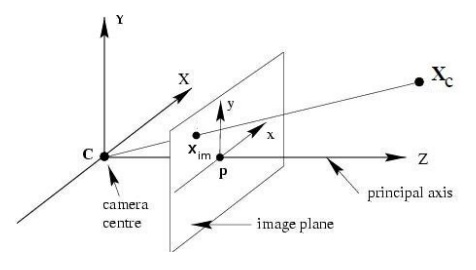
\includegraphics[scale=0.7]{perspective_projection}
	\caption{Γεωμετρική απεικόνιση της προοπτικής προβολής σημείου.}
	\label{fig:persp_proj}
\end{figure}

\begin{figure}
	\centering
	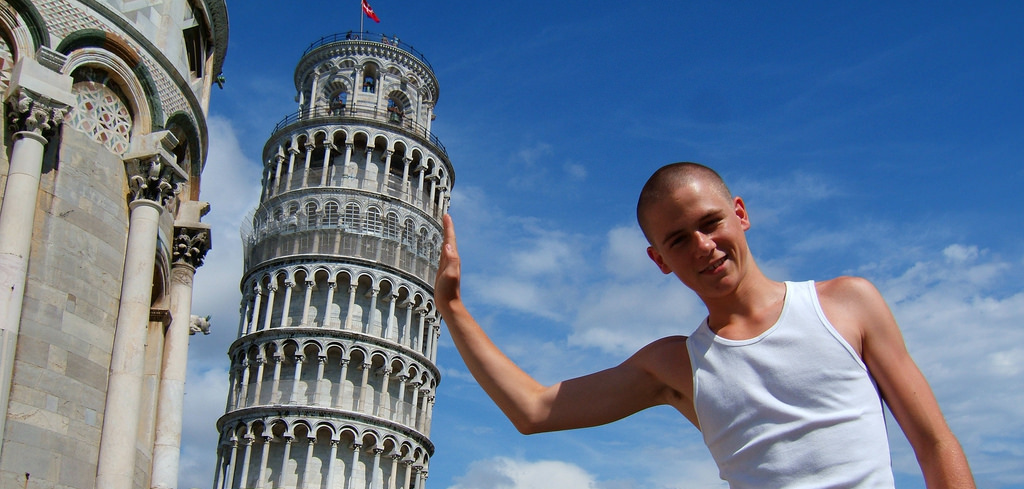
\includegraphics[scale=0.4]{illusion}
	\caption{Η ανάκτηση του βάθους είναι μια δύσκολη υπόθεση}
	\label{fig:illusion}
\end{figure}


%%%%%%%%%%%%%%%%%%%%%%%%%%%%%%%%%%%%%%%%%%%%%%%%%%%%%%%%%%%%%%%%%%%%%%%%%%%%%%%%%%%%%%%%%%%%%%%
\section{Γεωμετρία πολλαπλών προβολών}

Στην γεωμετρία πολλαπλών προβολών διαθέτουμε $n\geq2$ λήψεις της ίδιας τρισδιάστατης σκηνής. Θα μας απασχολήσει η περίπτωση των $n=2$ λήψεων.

\subsection{Προσδιορισμός τρισδιάστατης θέσης σημείου από δύο λήψεις}

Υποθέτουμε ότι:

\begin{enumerate}
	\item Ως σύστημα αναφοράς έχουμε ορίσει το σύστημα συντεταγμένων της μία εκ των δύο λήψεων. Την λήψη αυτή την ονομάζουμε λήψη αναφοράς και στην παρούσα εργασία επιλέγουμε να είναι η αριστερή.
	\item Γνωρίζουμε την ακριβή θέση και τον προσανατολισμό της έτερης (δεξιάς) λήψης στο χώρο. Συγκεκριμένα για τον πλήρη προσδιορισμό μιας λήψης ως προς μια άλλη χρειάζονται ένας πίνακα περιστροφής $R \in \mathbb{R}^{3\times 3} : \parallel R\parallel = 1$ και ένας πίνακας μετατόπισης $T \in  \mathbb{R}^3$. Αυτοί οι δύο πίνακες μαζί συνθέτουν έναν μετασχηματισμό \e affine, \g που τον συμβολίζουμε ως $g = (R,T)$. Εάν γνωρίζουμε τις συντεταγμένες ενός τυχαίου σημείου $P$ ως προς ένα ορισμένο σύστημα συντεταγμένων (στην περίπτωσή μας της αριστερής κάμερας), μπορούμε μέσω του μετασχηματισμού \e affine \g $g$ να βρούμε τις συντεταγμένες του $P$ ως το σύστημα συντεταγμένων της δεξιάς κάμερας. 
	\item Γνωρίζουμε τις ακριβείς θέσεις $ \mathbf{p_l}, \mathbf{p_r} \in \mathbb{R}^2$ στις οποίες έχει προβληθεί το \emph{ίδιο} σημείο του τρισδιάστατου χώρου $\mathbf{P}$.
\end{enumerate}

Με χρήση της σχέσης \ref{eq:simple_line}, προκύπτουν οι τρισδιάστατες \emph{ομοεπίπεδες} ευθείες $l_1$ και $l_2$ που αναλογούν στα σημεία $\mathbf{p_l}$ και $\mathbf{p_r}$. Το σημείο τομής των δύο ευθειών είναι η αρχική θέση $\mathbf{P}$ των σημείων $\mathbf{p_l}, \mathbf{p_r}$. Η διαδικασία αυτή, που φαίνεται στην εικόνα \ref{fig:triangulation}, ονομάζεται τριγωνοποίηση \e (triangulation). \g

\begin{figure}
	\centering
	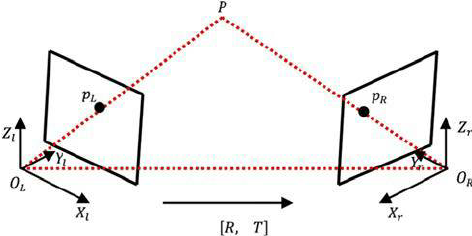
\includegraphics[scale=0.6]{triangulation}
	\caption{Τριγωνοποίηση}
	\label{fig:triangulation}
\end{figure}

\subsection{Το πρόβλημα της αντιστοίχησης}

Η μέθοδος της τριγωνοποίησης προϋποθέτει την γνώση των σημείων $\mathbf{p_l}$ και $\mathbf{p_r}$\footnote{στο εξής θα αναφέρονται ως "αντίστοιχα σημεία"}. Επομένως για την ανάκτηση της τρισδιάστατης θέσης ενός τυχαίου σημείου $\mathbf{p_l}$ απαιτείται η ανεύρεση του αντίστοιχου σημείου του $\mathbf{p_r}$ στην έτερη λήψη. Αυτή η αναζήτηση, που ονομάζεται "πρόβλημα αντιστοίχησης" \e (correspodence problem), \g είναι το κυρίαρχο πρόβλημα προς επίλυση σε κάθε εφαρμογή ανακατασκευής τρισδιάστατης πληροφορίας. 

Η αναζήτηση του "αντίστοιχου σημείου" δεν γίνεται κατά τυχαίο τρόπο στο σύνολο της έτερης λήψης. Αντίθετα η γεωμετρία των δύο προβολών περιορίζει την αναζήτησή του κατά μήκος μιας συγκεκριμένης ευθείας που βρίσκεται στο πέτασμα της έτερης λήψης. Η ευθεία αυτή ονομάζεται "επιπολική ευθεία". 

Αρχικά ορίζεται ο πίνακας \e essential matrix \g ως:

$$ E = [T]R \in \mathbb{R}^{3\times3}$$

Ως $[T]$ συμβολίζουμε τον $3\times 3$ πίνακα εξωτερικού γινομένου του διανύσματος $T$. Ο \e essential matrix \g υπολογίζεται άμεσα εφόσον γνωρίζουμε τον \e affine \g μετασχηματισμό $g = (R,T)$ και συμπυκνώνει την γεωμετρική συσχέτιση των σημείων $\mathbf{p_l}$ και $\mathbf{p_r}$ καθώς ικανοποιεί την σχέση:\footnote{Η απόδειξη της σχέσης \ref{eq:epipolar_constraint} παρατίθεται αναλυτικά στο παράρτημα \ref{appendix:epipolar_constraint_proof}}

\begin{equation} \label{eq:epipolar_constraint}
	\mathbf{p_r}^{T} E \mathbf{p_l} = 0
\end{equation}

Η σχέση \ref{eq:epipolar_constraint} ονομάζεται στερεοσκοπικός περιορισμός και από αυτήν προκύπτουν οι "επιπολικές ευθείες" κατά μήκος των οποίων βρίσκονται οι υποψήφιες θέσεις του "αντίστοιχου σημείου". Συγκεκριμένα εάν συμβολίσουμε με έναν πίνακα-γραμμή $l=[a \: b \: c]$ μια τυχαία ευθεία του επιπέδου $\mathbb{R}^2$\footnote{Έτσι ώστε το εσωτερικό γινόμενο του διανύσματος ευθείας $\mathbf{l}$ και ενός σημείου $\mathbf{p}$ να κάνει μηδέν μόνο όταν το σημείο ανήκει στην ευθεία} τότε ισχύει: 

\begin{itemize}

	\item το "αντίστοιχο σημείο" του $\mathbf{p_r}$ θα βρίσκεται πάνω στην επιπολική ευθεία $l_l = \mathbf{p_r}^{T} Ε$. Η ευθεία $l_l$ ορίζεται ως προς το σύστημα αναφοράς της λήψης 1 και βρίσκεται πάνω στο επίπεδο του πετάσματος της κάμερας 1, δηλαδή το επίπεδο $z = f$.
	\item το "αντίστοιχο σημείο" του $\mathbf{p_l}$ θα βρίσκεται πάνω στην επιπολική ευθεία $l_r = \mathbf{p_l} Ε$. Η ευθεία $l_r$ ορίζεται ως προς το σύστημα αναφοράς της λήψης 2 και βρίσκεται πάνω στο επίπεδο του πετάσματος της κάμερας 2, δηλαδή το επίπεδο $z = f$.
\end{itemize}

\begin{figure}
	\centering
	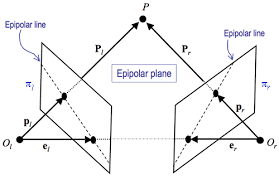
\includegraphics[scale=1]{epipolar_line}
	\caption{Επιπολικό επίπεδο και επιπολική ευθεία}
	\label{fig:epipolar_line}
\end{figure}


\subsection{Αντιστοίχηση στη στερεοσκοπική όραση}

\begin{figure}
	\centering
	\begin{subfigure}{0.48\textwidth}
		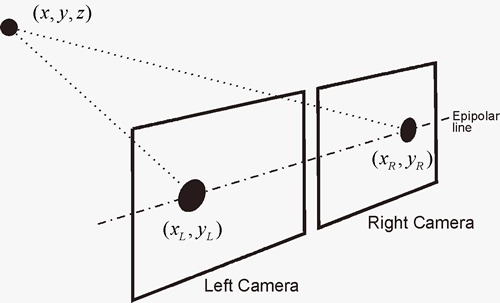
\includegraphics[width=\textwidth]{stereo_geometry}
		\caption{Στερεοσκοπική γεωμετρία}
		\label{fig:stereo_geometry}
	\end{subfigure}
	\begin{subfigure}{0.48\textwidth}
		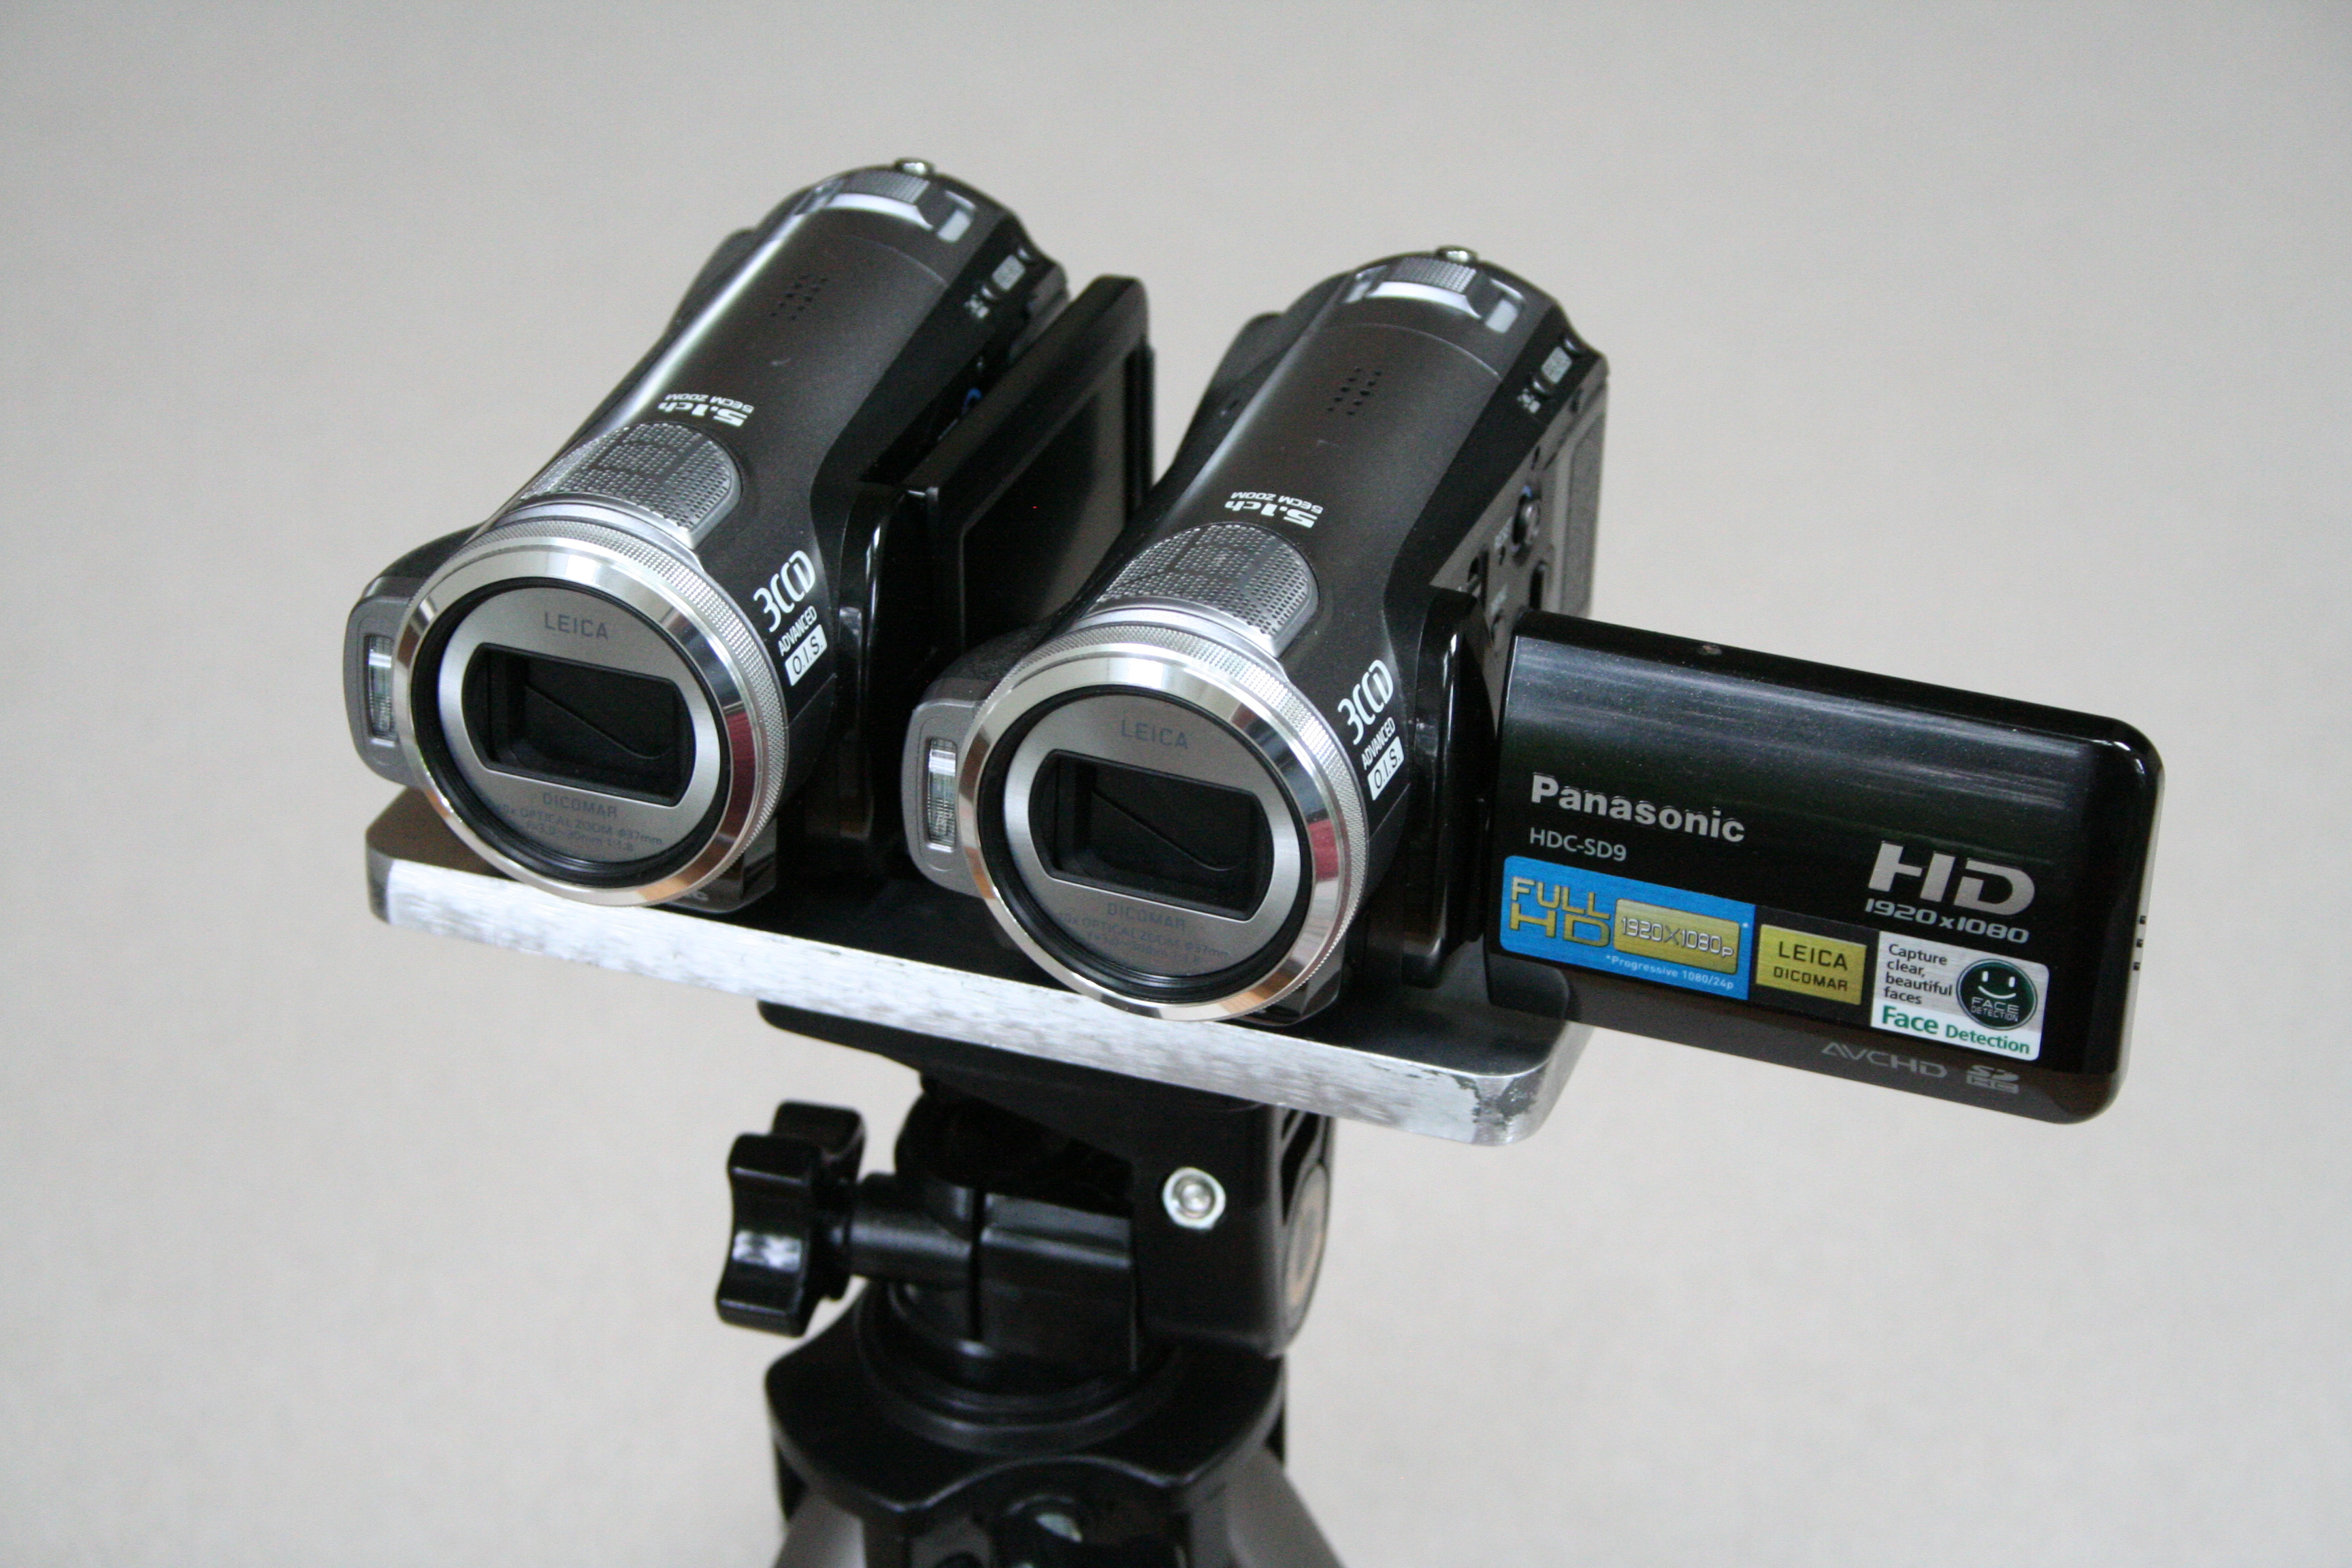
\includegraphics[width=\textwidth]{stereo_rig}
		\caption{Στερεοσκοπική διάταξη}
		\label{fig:stereo_rig}
	\end{subfigure}
\end{figure}

Στην στερεοσκοπική όραση, οι επιπολικές ευθείες είναι \emph{οριζόντιες}, όπως φαίνεται στην εικόνα \ref{fig:stereo_geometry}. Η προϋπόθεση αυτή ικανοποιείται είτε με φυσικό τρόπο, από την κατάλληλη τοποθέτηση στο χώρο των δύο λήψεων σε στερεοσκοπική διάταξη\footnote{Απόδειξη \ref{appendix:stereo_constraint_from_stereo_rig}}, είτε με την εφαρμογή κατάλληλων μετασχηματισμών σε ένα οποιοδήποτε ζεύγος εικόνων, διαδικασία που ονομάζεται ευθυγράμμιση\footnote{\g Απόδειξη \ref{appendix:stereo_constraint_from_rectification}} \e(rectification).\g

Επομένως σε ένα στερεοσκοπικό ζεύγος κάθε τυχαίο σημείο $\mathbf{p_l} = (x,y)$ της αριστερής λήψης:

\begin{itemize}
	\item είτε θα δεν θα βρίσκεται \textbf{πουθενά} στο πέτασμα της δεξιάς (εκτός οπτικού πεδίου της)
	\item είτε θα βρίσκεται στο σημείο $\mathbf{p_r} = (x-d,y)$, όπου $x-d\geq0\Leftrightarrow d \leq x$ \footnote{η περίπτωση όπου $d>x$ αναλογεί στην πρώτη υποπερίπτωση (εκτός οπτικού πεδίου της κάμερας 2)}
\end{itemize}
  
Η τιμή \e d, \g που εκφράζει την οριζόντια μετατόπιση του σημείου ανάμεσα στις δύο λήψεις, ονομάζεται παράλλαξη \e(disparity). \g Με γνωστά τα μεγέθη της στερεοσκοπικής διάταξης $f$, $B$ και της παράλλαξης $d$, ο υπολογισμός του βάθους $Ζ$ του τυχαίου σημείου $p$ είναι άμεσος:

\begin{equation} \label{eq:disp2depth}
	\left. 
		\begin{matrix}
			x_1 = -f\dfrac{X_1}{Z_1} \\
			x_2 = -f\dfrac{X_1 + B}{Z_1}
		\end{matrix}
	\right\} \Rightarrow
	Z_1 = \dfrac{fB}{x_1-x_2} = \dfrac{fB}{d}
\end{equation}

Γεωμετρικά η απόδειξη προκύπτει με κανόνα όμοιων τριγώνων φαίνεται στο σχήμα \ref{fig:disparity_proof}:

$$\dfrac{B}{Z} = \dfrac{(B+x_R)-x_L}{Z-f} \Rightarrow d = x_L - x_r = \dfrac{fB}{Z}$$

\begin{figure}
	\centering
	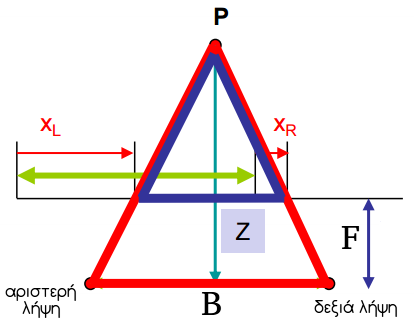
\includegraphics[scale=0.6]{disparity_proof.png}
	\caption{Γεωμετρική απόδειξη σχέσης βάθους και παράλλαξης.}
	\label{fig:disparity_proof}
\end{figure}



\subsection{Πεδίο παραλλάξεων και πεδίο βάθους}

Ο υπολογισμός της παράλλαξης \e d \g κάθε σημείου της εικόνας αναφοράς θα μας οδηγήσει σε έναν νέο πίνακα $D$ όμοιων διαστάσεων με την αρχική εικόνα $D \in \mathbb{R}^{height \times width}$, όπου σε κάθε του θέση θα είναι αποθηκευμένη η πληροφορία παράλλαξης του αντίστοιχου σημείου, όπως φαίνεται στο σχήμα \ref{fig:teddy}. Η παράλλαξη μετράται είτε σε $pixels$ είτε σε $cm$. Επί της ουσίας οι δύο μονάδες μέτρησης είναι ισοδύναμες καθώς η οριζόντια πλευρά του $pixel$ μετράται και αυτή σε $cm$. Στην παρούσα εργασία χρησιμοποιούμε ως μονάδα μέτρησης της παράλλαξης το $pixel$. Το πεδίο τιμών του χάρτη παραλλάξεων είναι το σύνολο $[0,width]$, διότι αν ένα σημείο αναλογεί σε παράλλαξη $> width$ τότε βρίσκεται εκτός οπτικού πεδίου της κάμερας 2.

Χάρτης βάθους \e (depth map) \g είναι ένας πίνακας $depth \in \mathbb{R}^{height \times width}$ που περιέχει την πληροφορία βάθους κάθε σημείου της εικόνας. Κατ' αντιστοιχία, επιλέγουμε ως μονάδα μέτρησης τα $pixels$. Το πεδίο τιμών του χάρτη παραλλάξεων είναι το σύνολο $[\dfrac{f\cdot b}{width},\infty]$, διότι αν ένα σημείο αναλογεί σε βάθος $< \dfrac{f\cdot b}{width}$ τότε βρίσκεται εκτός οπτικού πεδίου της κάμερας 2.

Η μετάβαση από το πεδίο των παραλλάξεων στο πεδίο του βάθους είναι '1-1' και αντιστρέψιμη. Οι δύο αναπαραστάσεις είναι ισοδύναμες.

$$disparity \xleftrightarrow[g^{-1}]{g} depth$$
$$ g:\mathbb{R}^{height \times width} \rightarrow \mathbb{R}^{height \times width} : depth = g(disparity) = \dfrac{fB}{disparity}$$
$$ g^{-1}:\mathbb{R}^{height \times width} \rightarrow \mathbb{R}^{height \times width} : disparity = g^{-1}(depth) = \dfrac{fB}{depth}$$

\begin{figure}
	\centering
	\begin{subfigure}{.32\textwidth}
		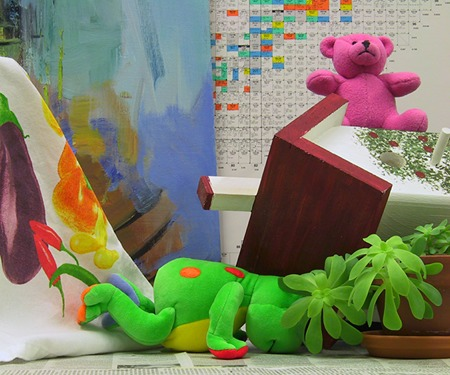
\includegraphics[width=\textwidth]{teddy_im2.jpg}
		\caption{Αριστερή λήψη}
	\end{subfigure}
	\begin{subfigure}{.32\textwidth}
		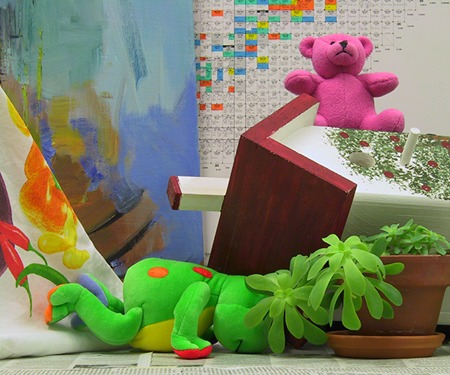
\includegraphics[width=\textwidth]{teddy_im6.jpg}
		\caption{Δεξιά λήψη}
	\end{subfigure}
	\begin{subfigure}{.32\textwidth}
		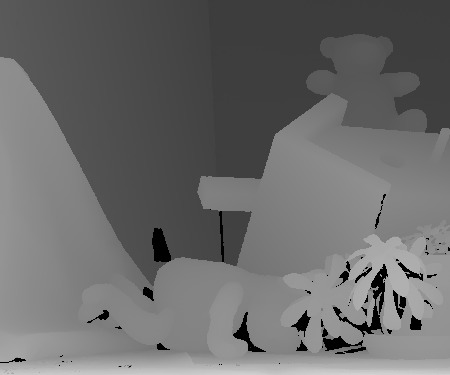
\includegraphics[width=\textwidth]{teddy_disp2.jpg}
		\caption{χάρτης παράλλαξης}
	\end{subfigure}
	\caption{παράδειγμα στερεοσκοπικής λήψης}
	\label{fig:teddy}
\end{figure}

%%%%%%%%%%%%%%%%%%%%%%%%%%%%%%%%%%%%%%%%%%%%%%%%%%%%%%%%%%%%%%%%%%%%%%%%%%%%%%%%%%%%%%%%%%%%%%%%%%%%%%%%%%%%%%%%%%%%%%%%%%%%
%%%%%%%%%%%%%%%%%%%%%%%%%%%%%%%%%%%%%%%%%%%%%%%%%%%%%%%%%%%%%%%%%%%%%%%%%%%%%%%%%%%%%%%%%%%%%%%%%%%%%%%%%%%%%%%%%%%%%%%%%%%%
%%%%%%%%%%%%%%%%%%%%%%%%%%%%%%%%%%%%%%%%%%%%%%%%%%%%%%%%%%%%%%%%%%%%%%%%%%%%%%%%%%%%%%%%%%%%%%%%%%%%%%%%%%%%%%%%%%%%%%%%%%%%

\section{Αρχές και περιορισμοί της στερεοσπικής αντιστοίχησης} \label{sec:stereo_constraints}


Για την διεκπεραίωση της στερεοσκοπικής αντιστοίχησης βασιζόμαστε σε υποθέσεις που οδηγούν σε αντίστοιχους περιορισμούς, κάποιοι εκ των οποίων έχουν καθολική κι άλλοι μερική ισχύ.\cite{pollefeys2004visual} Παραθέτουμε τους βασικότερους:

\begin{enumerate}[label=\textbf{\arabic*.}, ref={\arabic*}]
	\item \label{prop:stereo_contraint} \textbf{Στερεοσκοπικός περιορισμός \e (stereo constraint):} \g Όπως αποδείχθηκε στη σχέση \ref{eq:stereo_constraint}, η αναζήτηση του αντίστοιχου σημείου περιορίζεται αυστηρά και μόνο κατά μήκος της οριζόντιας επιπολικής ευθείας.
	\item \label{prop:disparity_continuity_constraint} \textbf{Περιορισμός συνέχειας/ασυνέχειας παράλλαξης \e (disparity continuity/discontinuity constraint):} \g
	\begin{itemize}
		\item Κατά μήκος συνεχών επιφανειών, οι τιμές της παράλλαξης είναι συνεχείς. Ο περιορισμός αίρεται μόνο στην περίπτωση όπου μια συνεχής επιφάνεια δημιουργεί εσωτερικά "κρυμμένα σημεία".\footnote{"Κρυμμένα σημεία" ονομάζουμε τα σημεία του χώρου που δεν είναι ορατά από μια λήψη.}
		\item Κατά μήκος ασυνεχών επιφανειών, οι τιμές της παράλλαξης είναι ασυνεχείς. Ο περιορισμός αίρεται στην περίπτωση που δύο ασυνεχείς επιφάνειες τυχαίνει να βρίσκονται στο ίδιο βάθος.\footnote{Όπως για παράδειγμα μια επιγραφή σε έναν τοίχο.}
	\end{itemize}
	Επομένως, ασυνέχειες στις τιμές της παράλλαξης συμβαίνουν είτε σε μεταβάσεις από μια επιφάνεια του χώρου σε μια άλλη, είτε αν δημιουργείται εντός μιας επιφάνειας εσωτερικό "κρυμμένο σημείο".
	\item \label{prop:uniqueness_contraint}\textbf{Περιορισμός μοναδικότητας \e (uniqueness constraint):} \g Σε αδιαφανή αντικείμενα, κάθε σημείο της μίας λήψης έχει το πολύ ένα σημείο αντιστοίχησης στην έτερη λήψη. Πιο συγκεκριμένα, ένα και μοναδικό, εάν είναι ορατό από την έτερη λήψη, και κανένα εάν δεν είναι ορατό.\footnote{η περίπτωση αυτή ονομάζεται απόκρυψη.} Έστω $\mathbf{p_1} \in I^{L}$, τότε 
	\[
	\mathbf{p_1}\xrightarrow{corresponds} \left\{
		\begin{array}{ll}
			\emptyset,\: \text{απόκρυψη} \\
            	\mathbf{p_2} \in I^{R},\: \text{αλλιώς}  \\
         \end{array}
          						\right.
    \]
    Στις περιοχές που είναι ορατές και από τις δύο λήψεις η παραπάνω σχέση γίνεται "1-1". Μπορούμε δηλαδή να αντιστοιχήσουμε μια αντιστρεπτή συνάρτηση $g$ μετάβασης ανάμεσα στα αντίστοιχα σημεία.
	\[
	p_1 \xLeftrightarrow[g^{-1}]{g} p_2
	\]
	Παραστατική απεικόνιση του περιορισμού μοναδικότητας παρουσιάζεται στο σχήμα \ref{fig:uniqueness_constraint}
	Ο περιορισμός παραβιάζεται μόνο σε σπάνιες περιπτώσεις διαφανών αντικειμένων, όπου δύο σημεία του τρισδιάστατου χώρου μπορεί να αποτυπώνονται ταυτόχρονα στο ίδιο σημείο του ενός πετάσματος και σε δύο διακριτά σημεία του έτερου. \ref{fig:transparent_object}
	\item \label{prop:ordering_contraint} \textbf{Περιορισμός διάταξης παραλλάξεων \e (ordering constraint):} \g Το σύνολο των σημείων που απαρτίζουν το είδωλο της επιφάνειας ενός αδιαφανούς αντικειμένου της τρισδιάστατης σκηνής, είναι διατεταγμένα κατά τον ίδιο τρόπο στις δύο λήψεις. Πρακτικά, ένα σημείο της επιφάνειες που αποτυπώθηκε πιο αριστερά από ένα άλλο στο ένα πέτασμα, δεν μπορεί να αποτυπωθεί αντίστροφα (πιο δεξιά) στο άλλο πέτασμα. \ref{fig:ordering_constraint_success} Ο ισχυρισμός καταρρέει αν μεταβούμε από την επιφάνεια ενός αντικειμένου σε αυτή ενός άλλου. \ref{fig:ordering_constraint_failure} Την περιοχή του χώρου εντός της οποίας αίρεται ο περιορισμός διάταξης, την αποκαλούμε "απαγορευμένη ζώνη" \e (forbidden zone). \g \ref{fig:forbidden_zone}
	\item \label{prop:stereo_constancy} \textbf{Σταθερότητα φωτισμού \e (color constancy):} \g Ο φωτισμός και ο χρωματισμός κάθε σημείου μιας σκηνής παραμένει αμετάβλητος σε κάθε θέση παρατήρησης της σκηνής. Ο ισχυρισμός αυτός ισχύει για τις λαμπερτιανές επιφάνειες που προκαλούν διάχυση, αναιρείται όμως όταν η σκηνή περιλαμβάνει μη-λαμπερτιανές (λείες ή διαφανείς επιφάνειες) που προκαλούν φαινόμενα κατοπτρικής ανάκλασης και διάθλασης.
	\item \label{prop:disparity_limit} \textbf{Όριο μέγιστης παράλλαξης \e (disparity limit):} \g Η μέγιστη δυνατή παράλλαξη του τυχαίου σημείου $p_1 = (x,y)$ της αριστερής κάμερας είναι η $d = x$, τιμή μεταβλητή ανάλογα με την τετμημένη του μελετούμενου σημείου. Σε κάθε περίπτωση η πιθανή παράλλαξη δεν μπορεί να υπερβαίνει το πλάτος της εικόνας $d \in [0,width]$. Πολλές φορές θέτουμε ένα, σχετικά αυθαίρετο, αυστηρότερο όριο ως μέγιστη παράλλαξη $d_{max}$, όταν δεν μας ενδιαφέρει ο ακριβής υπολογισμός του βάθους αντικειμένων που βρίσκονται πιο κοντά από το όριο αυτό. Το επίπεδο $Z = Z_{min}$ θέτει έναν κόφτη πέρα του οποίου όλα τα αντικείμενα χαρακτηρίζονται ως "πολύ κοντινά". Η σύμβαση του μέγιστου ορίου παράλλαξης έχει το σημαντικό πλεονέκτημα της μείωσης της υπολογιστικής πολυπλοκότητας.
\end{enumerate}

Θα μπορούσαμε να ομαδοποιήσουμε τους περιορισμούς 2, 3, 4 και 5 σε μια πιο ενιαία και ασαφή περιγραφή, αυτήν της "ομοιότητας γειτονιάς" \e(patches similarity). \label{prop:patches_similarity} \g Η "ομοιότητα γειτονιάς", εγκολπώνοντας τους παραπάνω περιορισμούς, υποθέτει ότι μια δεδομένη περιοχή της τρισδιάστατης σκηνής θα έχει \textit{παρόμοια} προβολή (σχήμα, χρώμα, μορφή, υφή) στα πετάσματα των δύο καμερών. Με δεδομένη αυτή την υπόθεση, θα αναζητήσουμε ακολούθως μετρικές ομοιότητας ώστε να αξιολογήσουμε την ομοιότητα περιοχών γύρω από τα σημεία ενδιαφέροντος και να "ταιριάξουμε" τα πλέον όμοια, δημιουργώντας τον ζητούμενο πίνακα παράλλαξης.

\begin{figure}
	\centering
	\begin{subfigure}{.6\textwidth}
		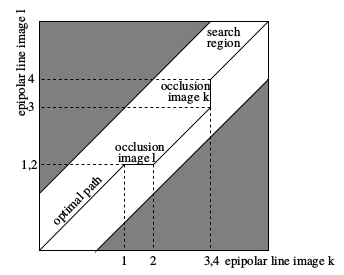
\includegraphics[width=\textwidth]{uniqueness1.png}
	\end{subfigure}
	\begin{subfigure}{.6\textwidth}
		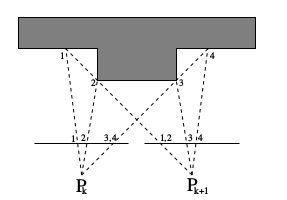
\includegraphics[width=\textwidth]{uniqueness2.png}
	\end{subfigure}
	\caption{Περιορισμός μοναδικότητας. Στο γράφημα ο οριζόντιος άξονας είναι η επιπολική γραμμή της αριστερής λήψης, ενώ ο κάθετος της δεξιάς. Παρατηρούμε ότι στις περιοχές που δεν υφίσταται απόκρυψη, δηλαδή μέχρι το σημείο 1, ανάμεσα στα σημεία 2,3 και μετά το σημείο 4, η σχέση που συνδέει τα αντίστοιχα σημεία είναι "1-1". Αντιθέτως στα σημεία που υπάρχει απόκρυψη για κάποια από τις δύο λήψεις, δηλαδή στις περιοχές ανάμεσα στα σημεία 1,2 και 3,4, η σχέση δεν είναι αντιστρεπτή.}
	\label{fig:uniqueness_constraint}
\end{figure}

\begin{figure}
	\centering
	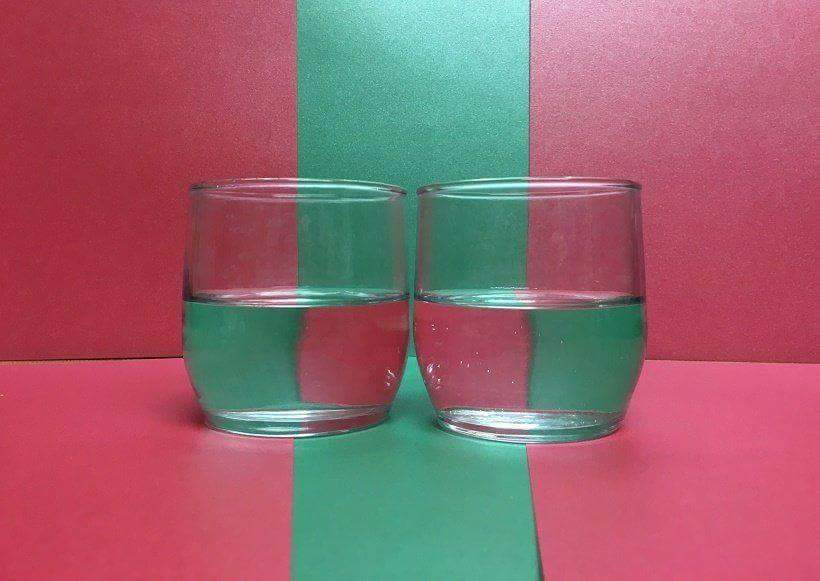
\includegraphics[width=0.5\textwidth]{transparent_object.jpg}
	\caption{Τα διάφανα αντικείμενα παραβιάζουν τον περιορισμό μοναδικότητας.}
	\label{fig:transparent_object}
\end{figure}

\begin{figure}
	\centering
	\begin{subfigure}{.49\textwidth}
		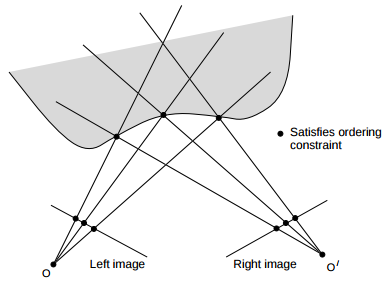
\includegraphics[width=\textwidth]{ordering_constraint.png}
		\caption{Περιορισμός διάταξης σε συνεχείς αδιαφανείς επιφάνειες}
		\label{fig:ordering_constraint_success}
	\end{subfigure}
	\begin{subfigure}{.49\textwidth}
		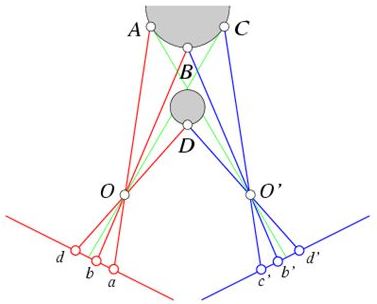
\includegraphics[width=\textwidth]{ordering_constraint_failure.png}
		\caption{Ο περιορισμός διάταξης αίρεται σε ασυνεχείς επιφάνειες}
		\label{fig:ordering_constraint_failure}
	\end{subfigure}
	\begin{subfigure}{.49\textwidth}
		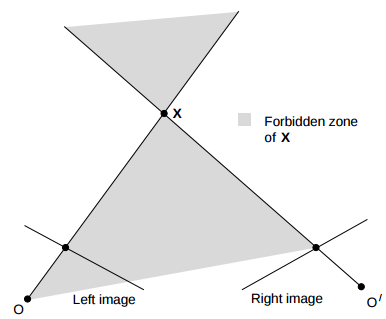
\includegraphics[width=\textwidth]{forbidden_zone.png}
		\caption{Απαγορευμένη περιοχή: οποιοδήποτε σημείο εντός της σκιασμένης περιοχής αναιρεί τον περιορισμό διάταξης παραλλάξεων}
		\label{fig:forbidden_zone}
	\end{subfigure}
	\caption{Περιορισμός διάταξης παραλλάξεων}
	\label{fig:ordering_constraint}
\end{figure}

%%%%%%%%%%%%%%%%%%%%%%%%%%%%%%%%%%%%%%%%%%%%%%%%%%%%%%%%%%%%%%%%%%%%%%%%%%%%%%%%%%%
%%%%%%%%%%%%%%%%%%%%%%%%%%%%%%%%%%%%%%%%%%%%%%%%%%%%%%%%%%%%%%%%%%%%%%%%%%%%%%%%%%%

\section{Μελέτη φαινομένων που αμφισβητούν τους περιορισμούς της στερεοσπικής αντιστοίχησης} \label{sec:stereo_constraints_violation}

Η υπόθεση της "ομοιότητας γειτονιάς" δεν έχει καθολική ισχύ. Εξ' ορισμού η προοπτική προβολή είναι μια πράξη μετασχηματισμού που αλλοιώνει το σχήμα του προβαλλόμενου αντικειμένου. Οι διαφορετικές θέσεις λήψης δημιουργούν διαφορετικά προβαλλόμενα είδωλα. Για αυτόν τον λόγο διαχωρίζουμε τα προβλήματα της στερεοσκοπικής αντιστοίχησης σε δύο μεγάλες κατηγορίες, στα προβλήματα μικρής και μεγάλης απόστασης βάσης \e (small and wide baseline stereo rig problems). \g Η βάση αναφέρεται στην οριζόντια απόσταση \e B (baseline) \g των δύο λήψεων. Στα προβλήματα μεγάλης απόστασης βάσης τα δύο είδωλα του ίδιου τρισδιάστατου αντικειμένου αποκλίνουν έντονα σε σχήμα, χρώμα και μορφή. Η απόκλιση οξύνεται κατ' αναλογία της αύξησης του μεγέθους \e B. \g \ref{fig:wide_baseline}
Στα προβλήματα μικρής απόστασης βάσης, που μας απασχολούν στην παρούσα εργασία, το φαινόμενο της σχηματικής, χρωματικής και μορφολογικής αλλοίωσης είναι αρκετά μειωμένο, όπως παρατηρούμε και στις εικόνες \ref{fig:small_baseline} \ref{fig:teddy}, χωρίς βέβαια να εξαφανίζεται πλήρως \ref{fig:perspective_transformation}. Επομένως είναι αρκετά βάσιμο να στηριχτούμε στην "ομοιότητα γειτονιάς" σε ένα ικανοποιητικό υποσύνολο των περιοχών της εικόνας. Σε συγκεκριμένες θέσεις παρατηρούνται φαινόμενα που αναιρούν ευθέως την παραπάνω υπόθεση, και κατ' επέκταση τις τέσσερις βασικές υποθέσεις που έχει στηριχτεί. Παρακάτω παραθέτουμε μια συνοπτική ανάλυση των φαινομένων αυτών:

\begin{enumerate}[label=\textbf{\arabic*.}, ref={\arabic*}]
	\item \label{prop:occlusions} \textbf{Αποκρύψεις \e(Occlusions):\g} Η έστω και μικρή μετατόπιση στη γωνία θέασης δημιουργεί περιοχές του \e 3D \g χώρου που είναι ορατές μόνο από τη μία εκ των δύο λήψεων, όπως παρατηρούμε στο σχήμα \ref{fig:occlusion}. Οι περιοχές αυτές εντοπίζονται συνήθως σε ασυνέχειες βάθους, δηλαδή σε σημεία που μεταβαίνουμε από ένα αντικείμενο σε ένα άλλο και παραβιάζουν ολοκληρωτικά την υπόθεση της "ομοιότητας γειτονιάς" \ref{fig:occlusion1}. Στις περιοχές αυτές πρέπει να δοθούν τιμές παράλλαξης εντός του διαστήματος τιμών $[D_L, D_R]$, όπου $D_L, D_R$ οι τιμές παράλλαξης των σημείων που βρίσκονται εκατέρωθεν της κρυμμένης περιοχής. Βέλτιστα η μεταβολή των τιμών παράλλαξης εντός της κρυμμένης περιοχής πρέπει να ακολουθεί μια γραμμική μεταβολή από το $D_L$ στο $D_R$, δηλαδή $d = D_L + (D_R - D_L)\dfrac{j - j_L}{j_R - j_L}$, όπου $j$ συμβολίζει την οριζόντια θέση και $D$ την τιμή της παράλλαξης.

	\item \label{prop:foreshortening_effect}\textbf{Φαινόμενο αυξομείωσης αποστάσεων και εμβαδών \e(Foreshortening effect):\g} Η προοπτική προβολή δεν κρατάει αναλλοίωτες τις αποστάσεις και τα εμβαδά. Το φαινόμενο της αυξομείωσης δημιουργεί διπλό πρόβλημα. Αφενός παραβιάζει την υπόθεση "ομοιότητας γειτονιάς", αφετέρου καθιστά και την αντιστοίχηση μη αντιστρεπτή καθώς $n \: pixels$ της μιας λήψης αντιστοιχούνται σε $m\neq n \: pixels$ της έτερης, παρ' ότι το αντικείμενο είναι \emph{απόλυτα ορατό και από τις δύο λήψεις}. \ref{fig:foreshortening}
	
	\item \label{prop:photometric_variations}\textbf{Αλλοιώσεις φωτισμού}: Ο όρος φωτισμός περιγράφει την διαδικασία υπολογισμού της έντασης της φωτεινής ακτινοβολίας που προσλαμβάνει ο θεατής, που στην περίπτωσή μας είναι οι στερεοσκοπικές κάμερες. Η φωτεινή ακτινοβολία, δηλαδή το εγκάρσιο κύμα του ορατού φωτός που προσπίπτει στο πέτασμα της κάμερας, μπορεί να έχει προέλθει από τέσσερα φυσικά φαινόμενα: αυτοφωτισμό, ανάκλαση, διάθλαση και διάχυση. Εκ των τεσσάρων αυτών φαινομένων, η κατοπτρική ανάκλαση και η διάθλαση δημιουργούν φωτισμό που διαφέρει ανάλογα με την θέση του θεατή. Το φαινόμενο αυτό ονομάζεται μη λαμπερτιανό φαινόμενο φωτισμού \e(non-lambertian lighting effect)\g και οι επιφάνειες που το προκαλούν ονομάζονται μη λαμπερτιανές \e(non-lambertian) \g επιφάνειες. Παραθέτουμε επιλεκτικά κάποιες περιπτώσεις:
	\begin{enumerate}
		\item \textbf{Κατοπτρικές ανακλάσεις:} Σε αυτήν την περίπτωση μια μη λαμπερτιανή επιφάνεια (π.χ. καθρέπτης) αποτυπώνει στο πέτασμα της κάμερας το είδωλο ενός τρίτου αντικείμενου το οποίο κατοπτρίζει. Το είδωλο του τρίτου αντικειμένου, που τελικά αποτυπώνεται στον φακό, υφίσταται μεγάλες αλλοιώσεις ακόμα και σε μικρές μεταβολές της θέσης του θεατή. \ref{fig:specular_reflection}
Το παραπάνω πολύ δύσκολα αντιμετωπίσιμο φαινόμενο είναι σχετικά σπάνιο. Μια πιο συνηθισμένη εκδοχή του είναι ο εστιασμένος κατοπτρισμός μιας φωτεινής πηγής, που δημιουργεί αλλοιωμένη φωτεινότητα στα προβαλλόμενα είδωλα. \ref{fig:specularity}.
		\item \textbf{Φωτομετρικές αποκλίσεις \e(photometric variations): \g} Συνήθως δεν προκαλεί ολική αλλοίωση στα δύο είδωλα, αλλά μια απόκλιση κυρίως στη φωτεινότητα και στο χρώμα. Αν το φαινόμενο είναι πολύ έντονο, η μεγάλη απόκλιση στη διαφορά φωτεινότητας μπορεί να κάνει ακατάληπτο το σχήμα του ειδώλου \ref{fig:photometric_variation}. Έντονες φωτομετρικές αποκλίσεις μεταξύ των δύο λήψεων προκαλούν συχνά οι σκιάσεις.
	\end{enumerate}
\end{enumerate}

Υπάρχουν επίσης περιπτώσεις όπου ενώ η "ομοιότητα γειτονιάς" τηρείται, δημιουργούνται ιδιαίτερα μοτίβα που δημιουργούν σύγχυση σε μια απλή μετρική ομοιότητας:
\begin{enumerate}[label=\textbf{\arabic*.}, ref={\arabic*}]
	\item \label{prop:repetitice_patterns}\textbf{Επαναλαμβανόμενα μοτίβα, δομές και υφές\e(repetitive patterns, structures and textures):\g} αν το φωτογραφιζόμενο τοπίο εμφανίζει επαναλαμβανόμενα μοτίβα (όπως βιβλία σε μια βιβλιοθήκη, ρίγες μιας ζέβρας ή μια σκακιέρα) ή επαναλαμβανόμενες υφές (όπως μια εικόνα από πολλά τριαντάφυλλα) τότε έντονη "ομοιότητα γειτονιάς" εμφανίζεται σε περισσότερα από ένα σημεία στην έτερη εικόνα, προκαλώντας αδυναμία επιλογής της καταλληλότερης περιοχής για αντιστοίχηση. Μια μετρική ομοιότητας γειτονιών εμφανίζει σε αυτήν την περίπτωση πολλά τοπικά μέγιστα. \ref{fig:repetitive}
	\item \label{prop:uniform_regions}\textbf{Μεγάλες ομοιόμορφες περιοχές \e(uniform regions):\g} αν το εικονιζόμενο τοπίο χαρακτηρίζεται από μεγάλες ομοιόμορφες περιοχές, όπως για παράδειγμα ο ουρανός, ο τοίχος μιας πολυκατοικίας και πολλά άλλα, η "ομοιότητα γειτονιάς" παραμένει παρόμοια (κατά περιπτώσεις και τελείως ίδια) σε μεγάλο εύρος διαφορετικών παραλλάξεων. Η μετρική ομοιότητας μένει για πολλές διαδοχικές τιμές παράλλαξης κοντά στο ολικό μέγιστο.
\end{enumerate}

Τέλος, υπάρχουν προβλήματα που δημιουργούνται λόγω θορύβου που προστίθεται κατά την λήψη της φωτογραφίας από το στερεοσκοπικό ζεύγος, όπως για παράδειγμα στην διαφορετική εστίαση όπου δημιουργείται θόλωμα \e(blur)\g κατά δυαδικό τρόπο σε κάθε λήψη δυσκολεύοντας την ανίχνευση της ομοιότητας. \ref{fig:different_focus}

\begin{figure}
	\centering
	\begin{subfigure}{.49\textwidth}
		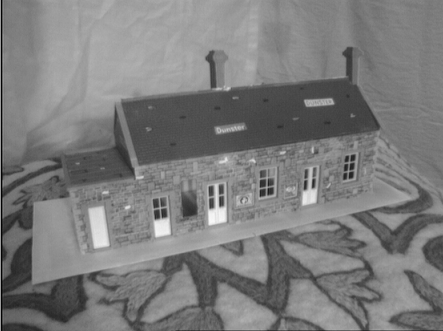
\includegraphics[width=\textwidth, height=0.55\textwidth]{wide_baseline_1_left.png}
		\caption{Αριστερή λήψη}
	\end{subfigure}
	\begin{subfigure}{.49\textwidth}
		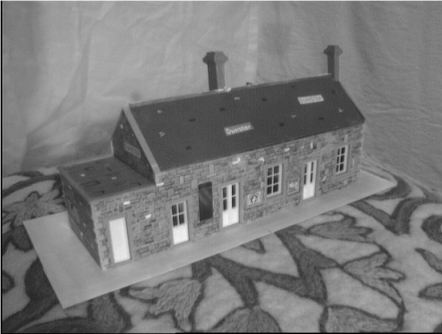
\includegraphics[width=\textwidth, height=0.55\textwidth]{wide_baseline_1_right.png}
		\caption{Δεξιά λήψη}
	\end{subfigure}
	\caption{Στερεοσκοπική λήψη μεγάλης απόστασης βάσης}
	\label{fig:wide_baseline}
\end{figure}

\begin{figure}
	\centering
	\begin{subfigure}{.49\textwidth}
		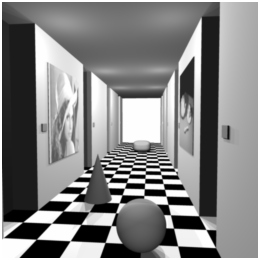
\includegraphics[width=\textwidth, height=0.55\textwidth]{small_baseline_1_left.png}
		\caption{Αριστερή λήψη}
	\end{subfigure}
	\begin{subfigure}{.49\textwidth}
		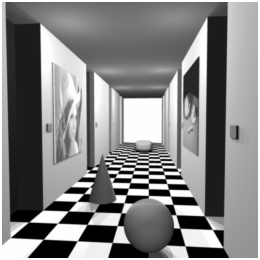
\includegraphics[width=\textwidth, height=0.55\textwidth]{small_baseline_1_right.png}
		\caption{Δεξιά λήψη}
	\end{subfigure}
	\caption{Στερεοσκοπική λήψη μικρής απόστασης βάσης}
	\label{fig:small_baseline}
\end{figure}

\begin{figure}
	\centering
	\begin{subfigure}{.49\textwidth}
		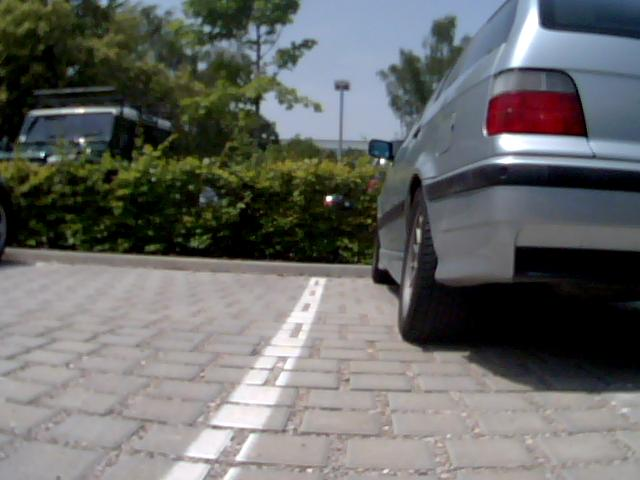
\includegraphics[width=\textwidth, height=0.55\textwidth]{perspective_transformation_l.png}
		\caption{Αριστερή λήψη}
	\end{subfigure}
	\begin{subfigure}{.49\textwidth}
		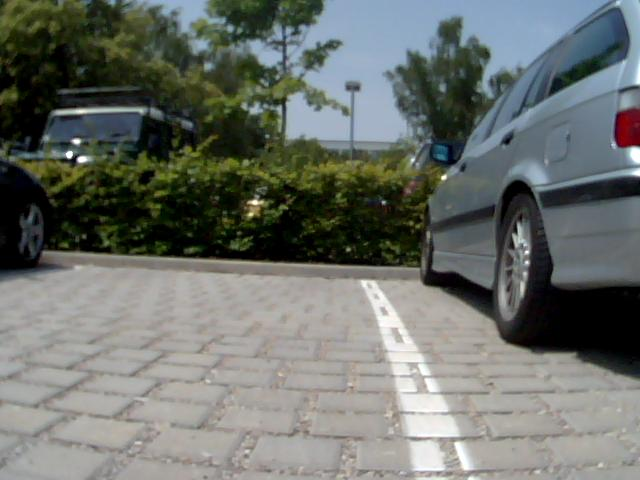
\includegraphics[width=\textwidth, height=0.55\textwidth]{perspective_transformation_r.png}
		\caption{Δεξιά λήψη}
	\end{subfigure}
	
	\begin{subfigure}{.49\textwidth}
		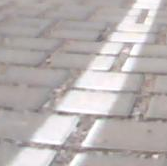
\includegraphics[width=\textwidth, height=0.55\textwidth]{perspective_transformation_l_crop.png}
		\caption{Αριστερή λήψη}
	\end{subfigure}
	\begin{subfigure}{.49\textwidth}
		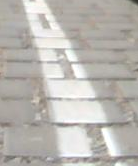
\includegraphics[width=\textwidth, height=0.55\textwidth]{perspective_transformation_r_crop.png}
		\caption{Δεξιά λήψη}
	\end{subfigure}
	\caption{Αλλοίωση των απεικονιζόμενων σχημάτων λόγω προοπτικής προβολής. Πηγή: \citep{TUMLesson}}
	\label{fig:perspective_transformation}
\end{figure}

\begin{figure}
	\centering
	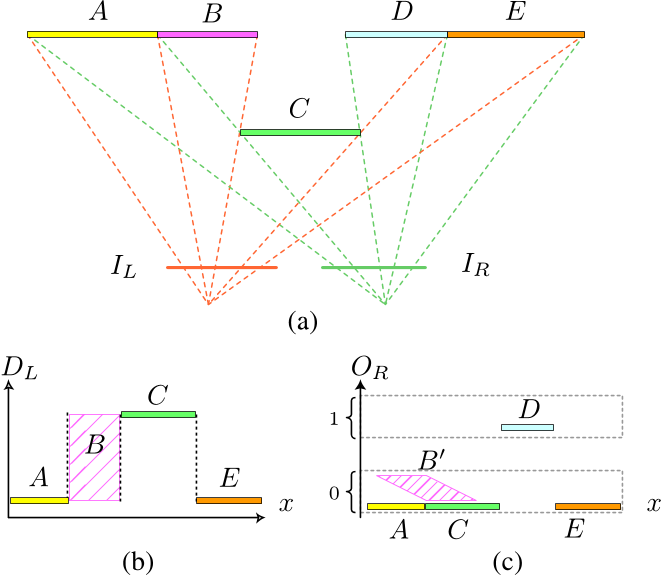
\includegraphics[width=0.8\textwidth]{occlusion_image.png}
	\caption{Ανάλυση φαινομένου απόκρυψης. (a) Στερεοσκοπικό ζεύγος εικόνων $I^L, I^R$ που αποτυπώνει μια σκηνή που περιλαμβάνει τα αντικείμενα \e A, B, C, D, E \g (b) Ο χάρτης παράλλαξης της αριστερής εικόνας. Παρατηρούμε ότι η παράλλαξη του αντικειμένου \e B \g είναι απροσδιόριστη λόγω απόκρυψης (δεν υπάρχει το είδωλό του στην έτερη λήψη). Υποχρεωτικά θα αντιστοιχηθεί είτε με το αντικείμενο \e A \g, είτε με το \e C \g, είτε θα επιμεριστεί σε δύο κομμάτια όπου αναλόγως θα αντιστοιχηθούν σε \e A \g και \e C \g. Γενικά, το αντικείμενο \e B \g θα λάβει τιμή παράλλαξης εντός του πεδίου $[D_A, D_C]$ (γ) Ο χάρτης απόκρυψης της δεξιάς εικόνας. Για την δεξιά εικόνα, το αντικείμενο \e D \g βρίσκεται σε απόκρυψη και όμοια με το (b) θα αντιστοιχηθεί είτε στο \e C \g είτε στο \e E \g.}
	\label{fig:occlusion}
\end{figure}

\begin{figure}
	\centering
	\begin{subfigure}{.49\textwidth}
		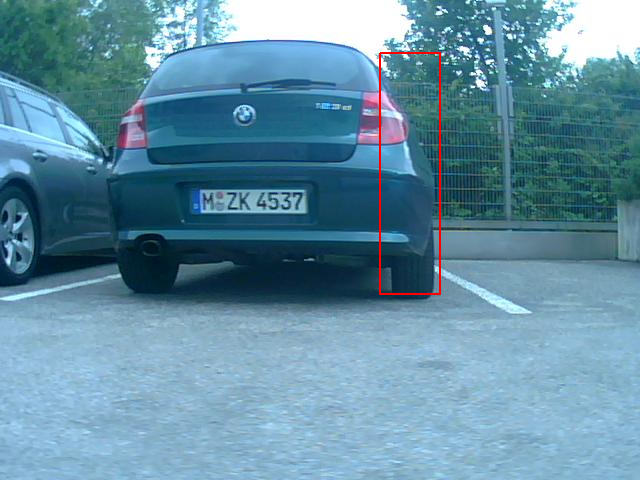
\includegraphics[width=\textwidth, height=0.55\textwidth]{occlusion_1_l.png}
		\caption{Αριστερή λήψη}
	\end{subfigure}
	\begin{subfigure}{.49\textwidth}
		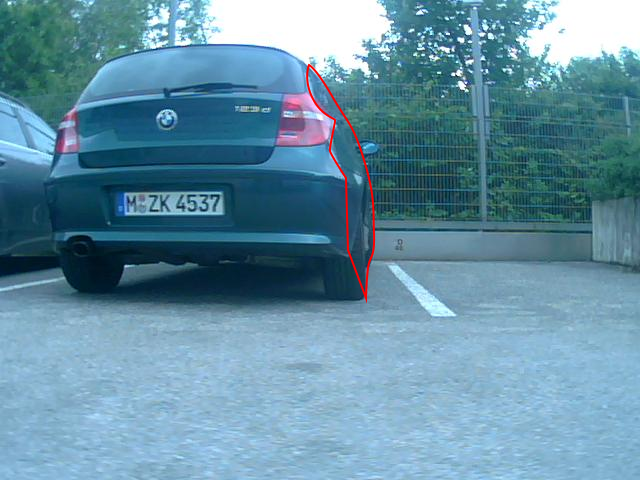
\includegraphics[width=\textwidth, height=0.55\textwidth]{occlusion_1_r.png}
		\caption{Δεξιά λήψη}
	\end{subfigure}
	
	\begin{subfigure}{.49\textwidth}
		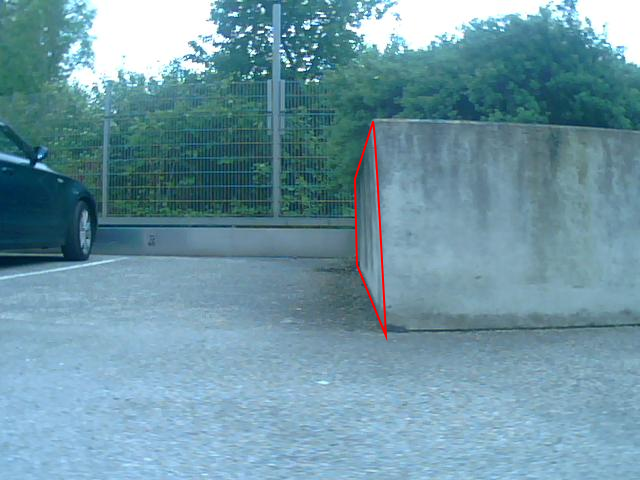
\includegraphics[width=\textwidth, height=0.55\textwidth]{occlusion_2_l.png}
		\caption{Αριστερή λήψη}
	\end{subfigure}
	\begin{subfigure}{.49\textwidth}
		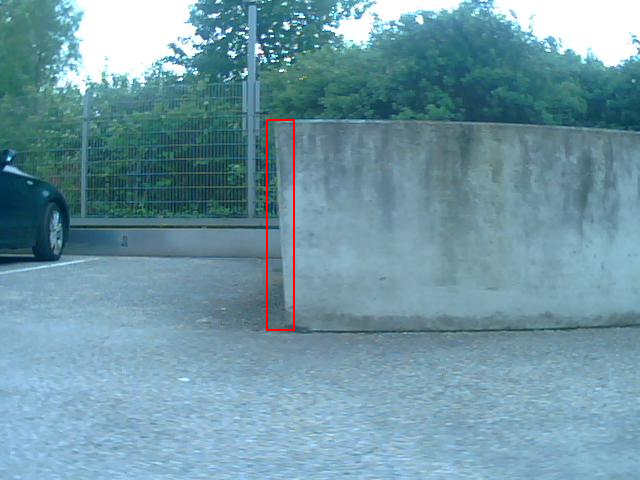
\includegraphics[width=\textwidth, height=0.55\textwidth]{occlusion_2_r.png}
		\caption{Δεξιά λήψη}
	\end{subfigure}
	\caption{Φαινόμενο απόκρυψης. Πηγή: \citep{TUMLesson}}
	\label{fig:occlusion1}
\end{figure}

\begin{figure}
	\centering
	\begin{subfigure}{.49\textwidth}
		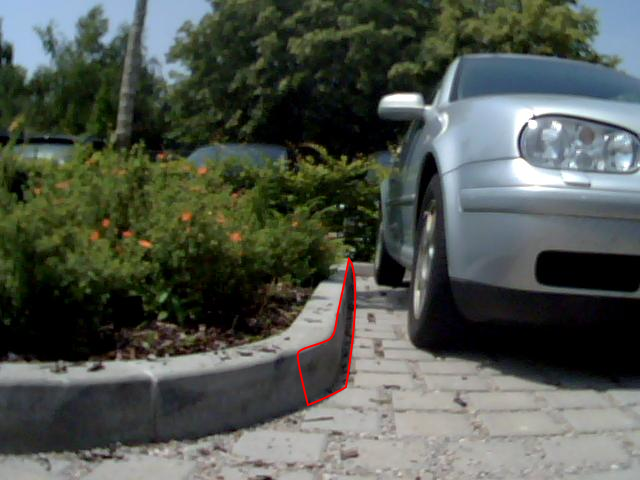
\includegraphics[width=\textwidth, height=0.55\textwidth]{foreshortening_l.png}
		\caption{Αριστερή λήψη}
	\end{subfigure}
	\begin{subfigure}{.49\textwidth}
		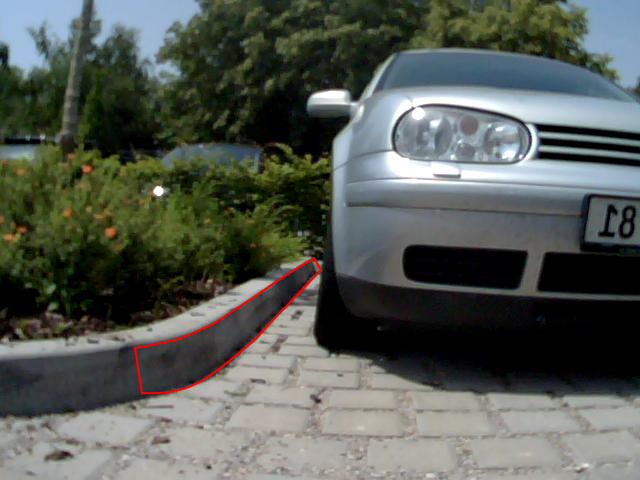
\includegraphics[width=\textwidth, height=0.55\textwidth]{foreshortening_r.png}
		\caption{Δεξιά λήψη}
	\end{subfigure}
	\caption{Φαινόμενο αυξομείωσης αποστάσεων και εμβαδών. Πηγή: \citep{TUMLesson}}
	\label{fig:foreshortening}
\end{figure}

\begin{figure}
	\centering
	\begin{subfigure}{.49\textwidth}
		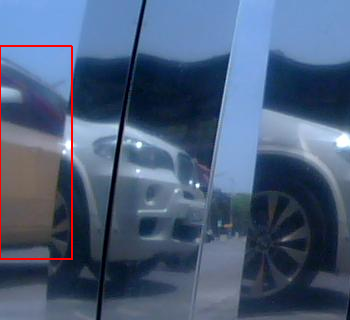
\includegraphics[width=\textwidth, height=0.55\textwidth]{specular_reflection_intense_l.png}
		\caption{Αριστερή λήψη}
	\end{subfigure}
	\begin{subfigure}{.49\textwidth}
		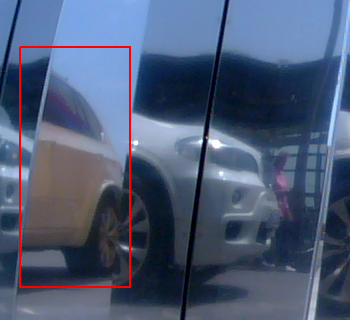
\includegraphics[width=\textwidth, height=0.55\textwidth]{specular_reflection_intense_r.png}
		\caption{Δεξιά λήψη}
	\end{subfigure}
	
	\begin{subfigure}{.49\textwidth}
		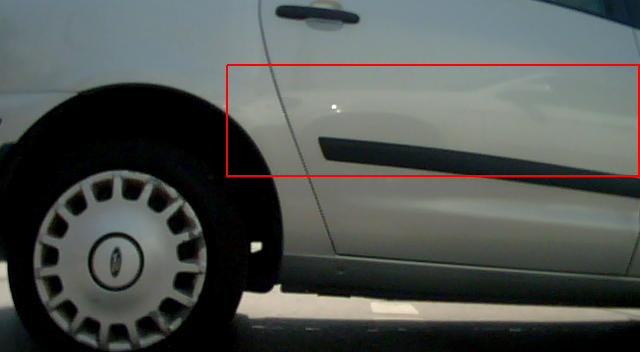
\includegraphics[width=\textwidth, height=0.55\textwidth]{specular_reflection_mild_l.png}
		\caption{Αριστερή λήψη}
	\end{subfigure}
	\begin{subfigure}{.49\textwidth}
		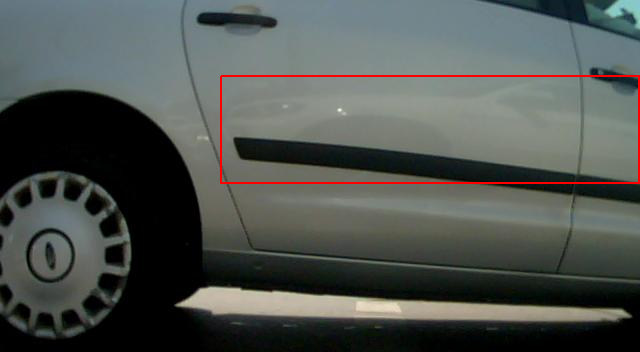
\includegraphics[width=\textwidth, height=0.55\textwidth]{specular_reflection_mild_r.png}
		\caption{Δεξιά λήψη}
	\end{subfigure}
	\caption{Φαινόμενο κατοπτρικής ανάκλασης τρίτου αντικειμένου. Πηγή: \citep{TUMLesson}}
	\label{fig:specular_reflection}
\end{figure}

\begin{figure}
	\centering
	\begin{subfigure}{.49\textwidth}
		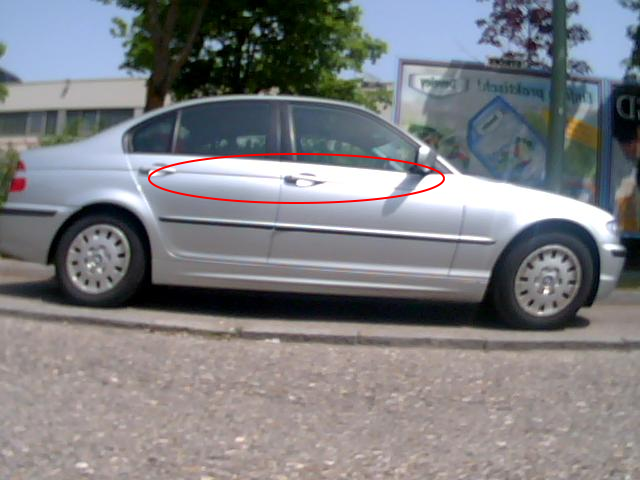
\includegraphics[width=\textwidth, height=0.55\textwidth]{specularity_1_l.png}
		\caption{Αριστερή λήψη}
	\end{subfigure}
	\begin{subfigure}{.49\textwidth}
		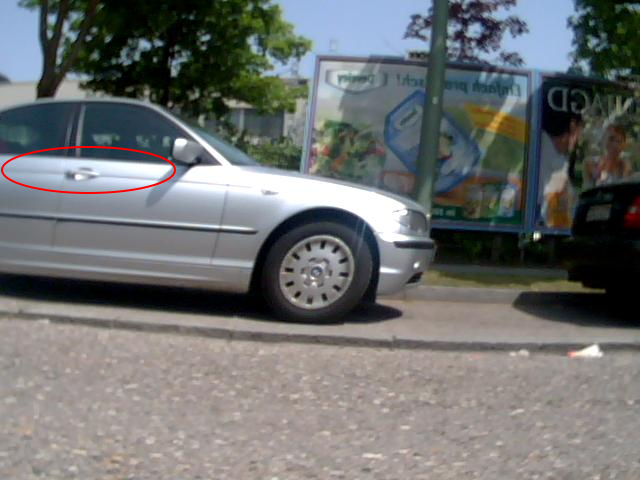
\includegraphics[width=\textwidth, height=0.55\textwidth]{specularity_1_r.png}
		\caption{Δεξιά λήψη}
	\end{subfigure}
	
	\begin{subfigure}{.49\textwidth}
		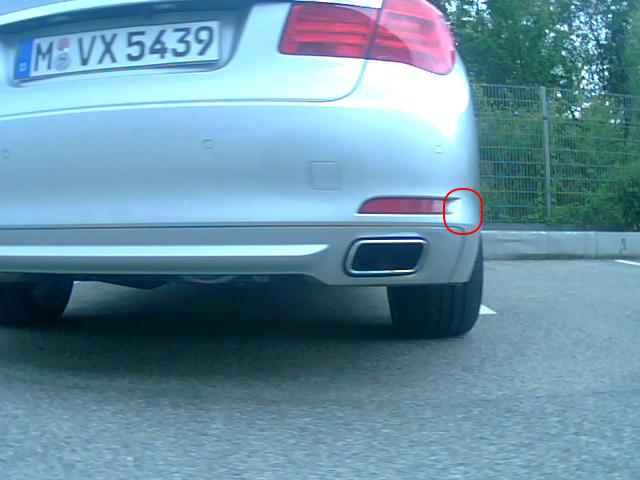
\includegraphics[width=\textwidth, height=0.55\textwidth]{specularity_2_l.png}
		\caption{Αριστερή λήψη}
	\end{subfigure}
	\begin{subfigure}{.49\textwidth}
		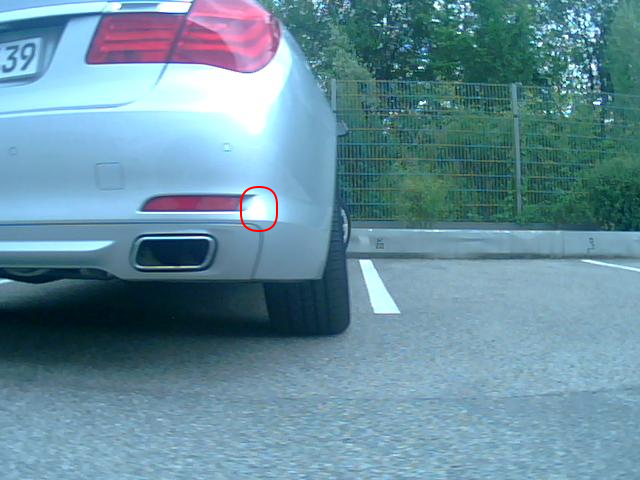
\includegraphics[width=\textwidth, height=0.55\textwidth]{specularity_2_r.png}
		\caption{Δεξιά λήψη}
	\end{subfigure}
	\caption{Φαινόμενο ανάκλασης φωτεινής πηγής. Πηγή: \citep{TUMLesson}}
	\label{fig:specularity}
\end{figure}

\begin{figure}
	\centering
	\begin{subfigure}{.49\textwidth}
		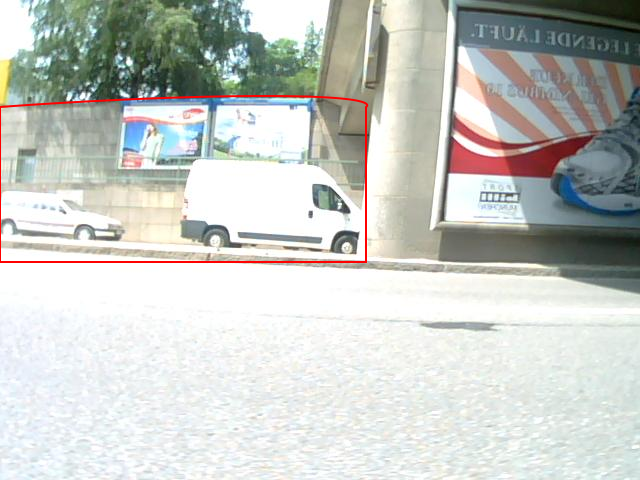
\includegraphics[width=\textwidth, height=0.55\textwidth]{photometric_variation_intense_l.png}
		\caption{Αριστερή λήψη}
	\end{subfigure}
	\begin{subfigure}{.49\textwidth}
		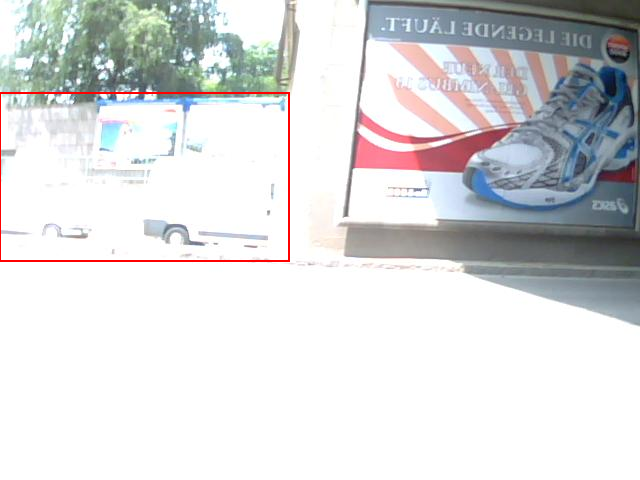
\includegraphics[width=\textwidth, height=0.55\textwidth]{photometric_variation_intense_r.png}
		\caption{Δεξιά λήψη}
	\end{subfigure}

	\begin{subfigure}{.49\textwidth}
		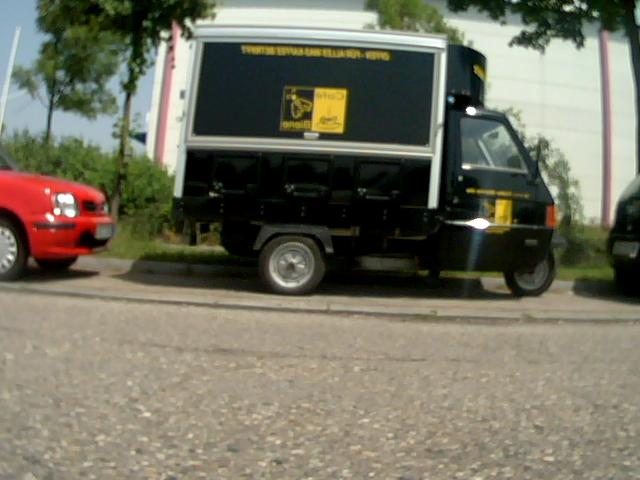
\includegraphics[width=\textwidth, height=0.55\textwidth]{photometric_variation_mild_l.png}
		\caption{Αριστερή λήψη}
	\end{subfigure}
	\begin{subfigure}{.49\textwidth}
		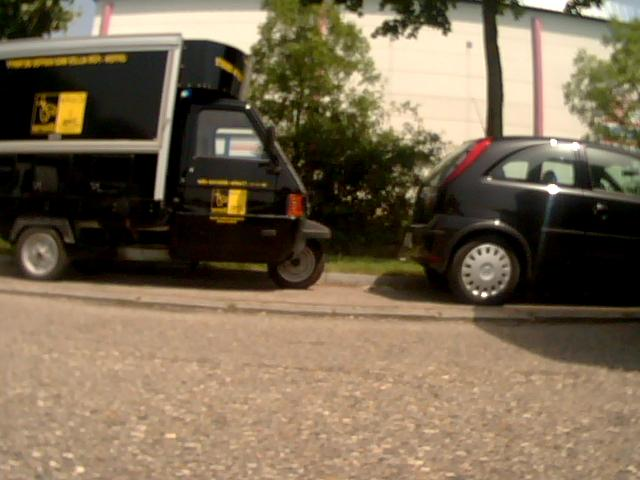
\includegraphics[width=\textwidth, height=0.55\textwidth]{photometric_variation_mild_r.png}
		\caption{Δεξιά λήψη}
	\end{subfigure}
	\caption{Φαινόμενο φωτομετρικής απόκλισης. Πηγή: \citep{TUMLesson}}
	\label{fig:photometric_variation}
\end{figure}

\begin{figure}
	\centering
	\begin{subfigure}{.3\textwidth}
		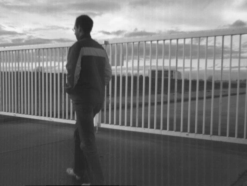
\includegraphics[width=\textwidth, height=0.55\textwidth]{repetitive1.png}
	\end{subfigure}
	\begin{subfigure}{.3\textwidth}
		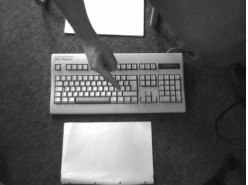
\includegraphics[width=\textwidth, height=0.55\textwidth]{repetitive2.png}
	\end{subfigure}
	\begin{subfigure}{.3\textwidth}
		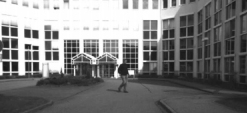
\includegraphics[width=\textwidth, height=0.55\textwidth]{repetitive4.png}
	\end{subfigure}
	\caption{Επαναλαμβανόμενα μοτίβα και υφές}
	\label{fig:repetitive}
\end{figure}

\begin{figure}
	\centering
	\begin{subfigure}{.49\textwidth}
		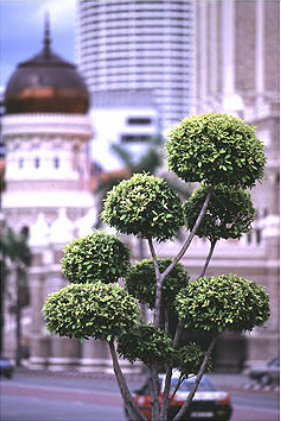
\includegraphics[width=\textwidth]{focus1.png}
		\caption{Αριστερή λήψη}
	\end{subfigure}
	\begin{subfigure}{.49\textwidth}
		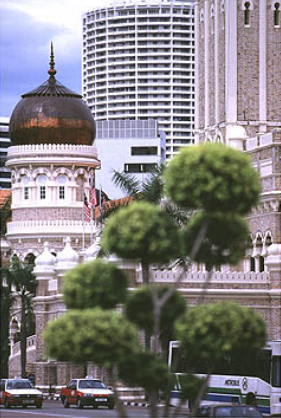
\includegraphics[width=\textwidth]{focus2.png}
		\caption{Δεξιά λήψη}
	\end{subfigure}
	\caption{Διαφορετική εστίαση σε κάθε λήψη}
	\label{fig:different_focus}
\end{figure}

Τα παραπάνω φαινόμενα αμφισβητούν, περισσότερο ή λιγότερο, τοπικά ή ολικά, τις αρχικές υποθέσεις στις οποίες βασίζονται οι μεθοδολογίες επίλυσης του προβλήματος της στερεοσκοπικής αντιστοίχησης απαιτώντας ειδική αντιμετώπιση.

%%%%%%%%%%%%%%%%%%%%%%%%%%%%%%%%%%%%%%%%%%%%%%%%%%%%%%%%%%%%%%%%%%%%%%%%%%%%%%%%%%%%%%%%%%%%%%%%%%%%%%%%%%%%%%%%%%%%%%%%%%%%
%%%%%%%%%%%%%%%%%%%%%%%%%%%%%%%%%%%%%%%%%%%%%%%%%%%%%%%%%%%%%%%%%%%%%%%%%%%%%%%%%%%%%%%%%%%%%%%%%%%%%%%%%%%%%%%%%%%%%%%%%%%%
%%%%%%%%%%%%%%%%%%%%%%%%%%%%%%%%%%%%%%%%%%%%%%%%%%%%%%%%%%%%%%%%%%%%%%%%%%%%%%%%%%%%%%%%%%%%%%%%%%%%%%%%%%%%%%%%%%%%%%%%%%%%

\section{Ανάλυση της στερεοσκοπικής αντιστοίχησης σε επιμέρους υποπροβλήματα}

Οι \e Scharstein et Szeliski \g \citep{in2002taxonomy} επιμερίζουν τους αλγορίθμους επίλυσης προβλημάτων στερεοσκοπικής όρασης σε 4 βήματα:

\begin{enumerate}
	\item Υπολογισμός κόστους αντιστοίχησης \e (matching cost computation) \g
	\item Άθροιση κόστους \e (cost aggregation) \g
	\item Υπολογισμός/βελτιστοποίηση χάρτη παράλλαξης \e (disparity computation/optimization) \g
	\item Διόρθωση χάρτη παράλλαξης \e (disparity refinement) \g
\end{enumerate}

Οι \e Hirschmuller et Scharstein \g \citep{hirschmuller2007evaluation} ομαδοποίησαν περαιτέρω την παραπάνω κατηγοριοποίηση προτείνοντας δύο μόνο βήματα:

\begin{enumerate}
	\item Αρχικοποίηση κόστους αντιστοίχισης \e (matching cost initialization) \g
	\item Στερεοσκοπική μέθοδος \e (Stereo method) \g
\end{enumerate}

Στην εργασία θα ακολουθήσουμε την ταξινόμηση των \e Hirschmuller et Scharstein. \g

%%%%%%%%%%%%%%%%%%%%%%%%%%%%%%%%%%%%%%%%%%%%%%%%%%%%%%%%%%%%%%%%%%%%%%%%%%%%%%%%%%%%%%%%%%%%%%%%%%%%%%%%%%%%%%%%%%%%%%%%%%%%
%%%%%%%%%%%%%%%%%%%%%%%%%%%%%%%%%%%%%%%%%%%%%%%%%%%%%%%%%%%%%%%%%%%%%%%%%%%%%%%%%%%%%%%%%%%%%%%%%%%%%%%%%%%%%%%%%%%%%%%%%%%%
%%%%%%%%%%%%%%%%%%%%%%%%%%%%%%%%%%%%%%%%%%%%%%%%%%%%%%%%%%%%%%%%%%%%%%%%%%%%%%%%%%%%%%%%%%%%%%%%%%%%%%%%%%%%%%%%%%%%%%%%%%%%

\section{Αρχικοποίηση κόστους αντιστοίχισης}

Στον παρών κεφάλαιο, όταν αναφερόμαστε σε σημείο $p=(x,y)$ της εικόνας εννοούμε το αντίστοιχο \e pixel. \g Επομένως, οι τιμές $x,y$ είναι διακριτές με πεδίο τιμών \e $[0,\ldots,width-1]$ \g και \e $[0,\ldots,height-1]$ \g αντίστοιχα. Κατά τον περιορισμό \ref{prop:disparity_limit} ορίζουμε ένα μέγιστο όριο στις υποψήφιες τιμές παράλλαξης που ερευνούμε και το ονομάζουμε $\mathtt{max\_disparity}$. Στόχος του παρόντος βήματος είναι για κάθε θέση $p$ της εικόνας αναφοράς και για πιθανή παράλλαξη $d$ να αναθέσουμε μια τιμή. Η τιμή αυτή θα προέλθει από την σύγκριση της γειτονιάς του $p$ με την αντίστοιχη γειτονιά του κάθε υποψήφιου σημείου $q = (x-d,y)$ στην έτερη λήψη. Αν η τιμή εκφράζει ομοιότητα, όσο μεγαλύτερη τόσο πιο όμοιες οι συγκρινόμενες γειτονιές, ενώ το αντίθετο ισχύει αν εκφράζει κόστος. Στην παρούσα εργασία επιλέγουμε η τιμή να εκφράζει κόστος. Συμβολίζουμε τη γειτονιά ενός σημείου $p$ με το σύμβολο $N_p$, και την ορίζουμε ως ένα τετράγωνο χωρίο με κέντρο το σημείο $p$. Το μέγεθος της γειτονιάς, δηλαδή η πλευρά του τετραγώνου, είναι μια ελεύθερη παράμετρος προς πειραματισμό.

Επομένως κατά το βήμα αυτό δημιουργούμε έναν τρισδιάστατο πίνακα κόστους:

$$ C(d,x,y) : \mathbb{Z}^3 \rightarrow \mathbb{R} : C(d,x,y) = cost(I^L(x,y),I^R(x-d,y))$$

Η συνάρτηση $cost$ είναι μια μετρική ομοιότητας. Παρακάτω παρατίθενται οι πιο γνωστές μετρικές που έχουν εφαρμοστεί:

\begin{itemize}
\item "Άθροισμα απόλυτων διαφορών" (\e sum of absolute differences - SAD):\citep{hannah1974computer}
$$ C(d,p) = -\sum_{q \in N_p} |I^L(q) - I^R(q-d)| $$ \g
Η πιο απλή μέθοδος, η οποία αξιοποιείται ως επίδοση βάσης. Βασίζεται στην παραδοχή ότι η φωτεινότητα μένει σταθερή κατά την προβολή μιας γειτονιάς σημείων του χώρου σε δυο διαφορετικές λήψεις.

\item "Άθροισμα τετραγώνων διαφορών" (\e sum of square differences - SSD):\citep{kanade1997development}
$$ C(d,p) = -\sum_{q \in N_p} { \left( I^L(q) - I^R(q-d) \right) }^2 $$ \g
Βασίζεται στις ίδιες παραδοχές με την μέθοδο \e SAD. \g Λόγω του τετραγώνου εμφανίζει εντονότερη πόλωση στα μεγάλα σφάλματα.

\item "Κανονικοποιημένη ετεροσυσχέτιση" ή "ομοιότητα συνημιτόνου":
\begin{equation*}
C(\mathbf{p}, d) = \frac{\sum_{\mathbf{q} \in \mathcal{N}_{\mathbf{p}}} I^L(\mathbf{q}) I^R(\mathbf{q} - \mathbf{d})}
{\sqrt{\sum_{\mathbf{q} \in \mathcal{N}_{\mathbf{p}}} I^L(\mathbf{q})^2 \sum_{\mathbf{q} \in \mathcal{N}_{\mathbf{p}}} I^R(\mathbf{q} - \mathbf{d})^2 }}.
\end{equation*}

\item Απόσταση \e Hamming \g σε μετασχηματισμό \e Census. \g Αρχικά εφαρμόζουμε στη γειτονιά $\mathcal{N}_{\mathbf{p}}$ τον μετασχηματισμό \e Census. \g Ο μετασχηματισμός αυτός συγκρίνει την φωτεινότητα κάθε σημείου της γειτονιάς $\mathcal{N}_{\mathbf{p}}$ με την φωτεινότητα του κεντρικού \e pixel, \g αποθηκεύοντας την ετικέτα $1$ αν είναι φωτεινότερο το περιφερειακό σημείο και $0$ σε αντίθετη περίπτωση:

\begin{equation*}
	\mathbf{c}_{i,j} = \begin{cases}
		1 & \text{εάν} \: |I(i,j) - I_c| \geqslant 0\\
		0 & \text{εάν} \: |I(i,j) - I_c| < 0
	\end{cases}
\end{equation*}

Έπειτα μετατρέπουμε τον πίνακα $\mathbf{c}_{i,j}$ σε ένα δυαδικό διάνυσμα $census(\mathbf{p})$ $n$ θέσεων, όσο και το μέγεθος της γειτονιάς. Τέλος εφαρμόζουμε την απόσταση \e Hamming \g στα διανύσματα $census$ των συγκρινόμενων περιοχών:

$$XNOR = census(I^L(\mathcal{N}_{\mathbf{p}}) \odot census(I^R(\mathcal{N}_{\mathbf{\mathbf{p} - \mathbf{d}}}) $$
$$C(\mathbf{p}, d) = XNOR\cdot XNOR$$
\end{itemize}

Έχουν προταθεί πολλές ακόμη μέθοδοι αρχικοποίησης του πίνακα κόστους. Το βήμα αυτό είναι το σημαντικότερο στην αλληλουχία βημάτων που καταλήγει στον υπολογισμό του χάρτη παράλλαξης και γι' αυτό η βιβλιογραφία είναι μεγάλη. Στο επόμενο κεφάλαιο θα δούμε πως με τη χρήση μηχανικής μάθησης μέσω τεχνητού νευρωνικού δικτύου, καταφέρνουμε την αρχικοποίηση πίνακα κόστους πολύ μεγαλύτερης ακρίβειας από αυτόν που πετυχαίνουν όλες οι παραπάνω μέθοδοι.

%%%%%%%%%%%%%%%%%%%%%%%%%%%%%%%%%%%%%%%%%%%%%%%%%%%%%%%%%%%%%%%%%%%%%%%%%%%%%%%%%%%%%%%%%%%%%%%%%%%%%%%%%%%%%%%%%%%%%%%%%%%%
%%%%%%%%%%%%%%%%%%%%%%%%%%%%%%%%%%%%%%%%%%%%%%%%%%%%%%%%%%%%%%%%%%%%%%%%%%%%%%%%%%%%%%%%%%%%%%%%%%%%%%%%%%%%%%%%%%%%%%%%%%%%
%%%%%%%%%%%%%%%%%%%%%%%%%%%%%%%%%%%%%%%%%%%%%%%%%%%%%%%%%%%%%%%%%%%%%%%%%%%%%%%%%%%%%%%%%%%%%%%%%%%%%%%%%%%%%%%%%%%%%%%%%%%%

\section{Στερεοσκοπική Μέθοδος \texorpdfstring{\e (stereo method) \g}{TEXT}}

Η αρχικοποίηση του όγκου κόστους $C$ περιέχει αρκετές λανθασμένες εκτιμήσεις, τοποθετημένες στα σημεία που αναιρούνται οι περιορισμοί της στερεοσκοπικής αντιστοίχησης (αποκρύψεις, φωτομετρικές αλλοιώσεις, ομοιόμορφες περιοχές κ.α.). Στην στερεοσκοπική μέθοδο, εφαρμόζουμε τεχνικές που βελτιώνουν τις αρχικές εκτιμήσεις, οδηγώντας σε πιο ακριβή τελικό χάρτη παράλλαξης.

Θα αξιοποιήσουμε κυρίως τις μεθόδους που χρησιμοποίησαν οι \e Mei et al. \g (2011) \cite{mei2011building} κι αναπροσάρμοσαν οι \e Zbontar et LeCun (2016) \g \cite{zbontar2016stereo}.

\subsection{Άθροιση κόστους σε περιοχή υποστήριξης}

Βασιζόμενοι στην υπόθεση "ομοιότητας γειτονιάς" (η οποία καταρρέει τοπικά σε ασυνέχειες βάθους), μπορούμε να αναθέσουμε σε κάθε \e pixel \g τον μέσο όρο των αρχικοποιημένων τιμών κόστους ολόκληρης της γειτονιάς του. Υποθέτουμε δηλαδή ότι αν ένα σημείο $\mathbf{p}$ έχει παράλλαξη $d$ τότε και τα γειτονικά του σημεία θα βρίσκονται σε ίδια ή κοντινή παράλλαξη, αρκεί να μη μεταβαίνουμε από ένα αντικείμενο σε ένα άλλο.

Το σχήμα και το μέγεθος της γειτονιάς, που στο εξής θα ονομάζουμε περιοχή υποστήριξης \e (support region) \g μπορούν να προσδιοριστούν με δύο τρόπους:

\begin{itemize}
	\item Ως μια ορθογώνια περιοχή προαποφασισμένου μεγέθους.
	\item Ως μια προσαρμοσμένη περιοχή, διαφορετική για κάθε σημείο $\mathbf{p}$.
\end{itemize}

\subsubsection{Ορθογώνια περιοχή}
Η περιοχή υποστήριξης είναι ένα τετράγωνο χωρίο το μέγεθος του οποίου επιλέγεται πειραματικά. Η επιλογή: 

\begin{itemize}
	\item μικρής περιοχής υποστήριξης προκαλεί ασάφειες (πολλές διαφορετικές τιμές παράλλαξης με παρόμοιο κόστος), καθώς δεν συνδυάζει αρκετή πληροφορία. Έτσι προκαλείται ένας χάρτης παράλλαξης αρκετά "τραχύς" με πολλές εξωκείμενες τιμές. \ref{fig:small_window}
	\item μεγάλης περιοχής υποστήριξης έχει τα αντίστροφα αποτελέσματα. Συνδυάζει αρκετή πληροφορία, δημιουργώντας λείο χάρτη παράλλαξης, αλλά αδυνατεί να εντοπίσει τις ακμές τις οποίες και θολώνει καθώς πάσχει σε περιοχές ασυνέχειας βάθους, όπου οι αποκρύψεις καταστρατηγούν την "ομοιότητα γειτονιάς". \ref{fig:large_window}
\end{itemize}

Η μαθηματική πράξη που υλοποιεί την παραπάνω διεργασία είναι η χωρική συνέλιξη με χωρικό φίλτρο μέσου όρου:

\begin{align*}
	\mathtt{for} \: \: & \mathtt{d = 0:max\_disparity} \\
	& C_{agg}(d,:,:) = C_{init}(d,:,:) \ast h
\end{align*}



όπου $C_{init}$ ο αρχικός πίνακας κόστους, $C_{agg}$ αυτός που προκύπτει μετά την συνέλιξη και $h$ το φίλτρο μέσου όρου.

Η παραπάνω πράξη μπορεί μάλιστα να εφαρμοστεί κατ' επανάληψη, που ισοδυναμεί βαθμιαία με συνέλιξη με γκαουσιανό φίλτρο μεγαλύτερων διαστάσεων, όπως αποδεικνύεται στο παράρτημα \ref{appendix:mean2gaussian}.

\begin{figure}
	\centering
	\begin{subfigure}{.33\textwidth}
		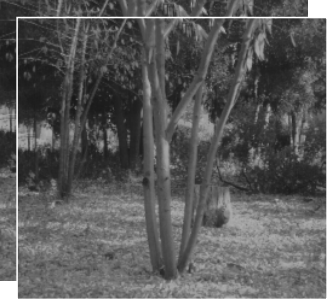
\includegraphics[width=\textwidth]{cost_aggregation1.png}
		\caption{στερεοσκοπικό ζεύγος}
	\end{subfigure}
	\begin{subfigure}{.33\textwidth}
		\includegraphics[width=\textwidth]{cost_aggregation2.png}
		\caption{μικρό παράθυρο $w=3$ pixels}
		\label{fig:small_window}
	\end{subfigure}
		\begin{subfigure}{.33\textwidth}
		\includegraphics[width=\textwidth]{cost_aggregation3.png}
		\caption{μεγάλο παράθυρο $w=20$ pixels}
		\label{fig:large_window}
	\end{subfigure}
	\caption{χάρτης παράλλαξης για μεταβλητό μέγεθος παραθύρου}
\end{figure}


\subsubsection{Προσαρμοσμένη περιοχή υποστήριξης}

Ο ορισμός ενιαίας περιοχής υποστήριξης για όλα τα σημεία προκαλεί τα παραπάνω προβλήματα. Επιθυμούμε την δημιουργία περιοχής υποστήριξης διαφορετικού μεγέθους και σχήματος ανά σημείο. Στόχος είναι η περιοχή υποστήριξης να μην περιλαμβάνει μεταβάσεις από ένα αντικείμενο σε ένα άλλο. Έτσι οι μέσοι όροι θα συνδυάζουν πληροφορία από γειτονικά \e pixels \g που ανήκουν στο ίδιο αντικείμενο και άρα έχουν ίδια ή παρόμοια τιμή παράλλαξης. 

Βασιζόμαστε στην υπόθεση ότι η μετάβαση από ένα αντικείμενο σε ένα άλλο αποτυπώνεται στο πέτασμα μέσω απότομης αλλαγής στη φωτεινότητα των \e pixels. \g \citep{lu2008anisotropic} Ακολουθώντας την μεθοδολογία που πρότειναν οι \e Zhang et al. (2009) \g \cite{zhang2009cross}, αντιστοιχίζουμε σε κάθε \e pixel \g τέσσερις τιμές που συγκροτούν έναν σταυρό. Συγκεκριμένα, οι τέσσερις τιμές $[v_{p}^-, v_{p}^+, h_{p}^-, h_{p}^+]$ δηλώνουν πόσο εκτείνεται ο σταυρός στις τέσσερις κατευθύνσεις: πάνω, κάτω - κάθετος άξονας - και αριστερά, δεξιά - οριζόντιος άξονας.

Αποφασίζουμε την τιμή των $[v_{p}^-, v_{p}^+, h_{p}^-, h_{p}^+]$ που αντιστοιχούν στο \e pixel \g $p$ ακολουθώντας δύο κριτήρια. Μετατοπιζόμαστε κατά μήκος της κάθε κατεύθυνσης όσο τηρούνται οι περιορισμοί: 

\begin{itemize}
	\item \e $|I(\mathbf{p}) - I(\mathbf{p'})| < \texttt{intensity\_threshold}$: \g η διαφορά στη φωτεινότητα μεταξύ του υπό εξέταση \e pixel \g $\mathbf{p}$ και του $\mathbf{p'}$ είναι μικρότερο ενός ορίου που θέτουμε ως παράμετρο. Όσο μικρότερη τιμή ορίου, τόσο αυξανόμενη ευαισθησία στην ανεύρεση συνόρου.			
	\item \e $\|\mathbf{p} - \mathbf{p'}\| < \texttt{distance\_threshold}$: \g η μέγιστη τιμή προς κάθε κατεύθυνση περιορίζεται από το όριο  \e $\texttt{distance\_threshold}$ \g επιβάλλοντας περιορισμό στο μέγιστο εμβαδό της περιοχής υποστήριξης.
\end{itemize}

Αφού υπολογιστούν οι τέσσερις τιμές \e $[v_{p}^-, v_{p}^+, h_{p}^-, h_{p}^+]  \forall \mathbf{p}$\g, η περιοχή υποστήριξης του \e$\mathbf{p}$ \g υπολογίζεται ως η ένωση των τιμών $[h_{p}^-, h_{p}^+]$ όλων των θέσεων \e$\mathbf{q}$ \g κατά μήκος του κάθετου άξονα του \e $\mathbf{p}$ \g, όπως φαίνεται στο σχήμα \ref{fig:cbca_cross}

Η τελική επιλογή περιοχής υποστήριξης πρέπει λαμβάνει υπ' όψη και την αντίστοιχη περιοχή στο αντίστοιχο \e pixel \g της έτερης λήψης. Επομένως, συμβολίζοντας \e $U^{L}(\mathbf{p})$ \g την περιοχή υποστήριξης στην αριστερή λήψη, \e $U^{R}(\mathbf{p})$ \g στην δεξιά, η τελική περιοχή υποστήριξης για την υπό εξέταση παράλλαξη $d$ είναι η: \e

\begin{gather*}
U_d(\mathbf{p}) = U^{L}(\mathbf{p}) \cup  U^{R}(\mathbf{p-d}) \Rightarrow\\
U_d(\mathbf{p}) = \{\mathbf{q} | \mathbf{q} \in U^L(\mathbf{p}), \mathbf{q}-\mathbf{d}
\in U^R(\mathbf{p}-\mathbf{d})\}
\end{gather*}\g

Στο σχήμα \ref{fig:cbca_tsukuba}, φαίνεται ότι η προσαρμοσμένη περιοχή υποστήριξης αποδίδει με ικανοποιητική ακρίβεια, καταφέρνοντας να περιορίσει τις περιοχές υποστήριξης εντός των ίδιων αντικειμένων και αποφεύγοντας την εμπλοκή εξωκείμενων τιμών στον υπολογισμό των μέσων όρων. 

Η υπολογιστική πολυπλοκότητα του υπολογισμού της γειτονιάς για κάθε σημείο είναι \e $O(H \cdot W \cdot \texttt{distance\_threshold})$, \g ενώ για την άθροιση του κόστους $O(H \cdot W \cdot D \cdot (2 \cdot \texttt{distance\_threshold})^2)$ 

\begin{figure}
	\centering
	\includegraphics[width=0.5\textwidth]{cbca_cross.png}
	\caption{παράδειγμα δημιουργίας περιοχής υποστήριξης τυχαίου \e pixel $\mathbf{p}$ \g. Αφού, υπολογιστούν οι τιμές $[v_{p}^-, v_{p}^+, h_{p}^-, h_{p}^+]$ υπολογίζονται οι οριζόντιοι άξονες όλων των θέσεων \e $\mathbf{q}$ \g κατά μήκος του κάθετου άξονα}
	\label{fig:cbca_cross}
\end{figure}

\begin{figure}
	\centering
	\includegraphics[width=1\textwidth]{cbca_tsukuba.png}
	\caption{εφαρμογή μεθόδου υπολογισμού προσαρμόσιμων περιοχών υποστήριξης.}
	\label{fig:cbca_tsukuba}
\end{figure}

\subsection{Ημικαθολική αντιστοίχηση \texorpdfstring{\e (semi-global matching) \g}{TEXT}}

Η μέθοδος άθροισης κόστους σε περιοχές υποστήριξης του προηγούμενο κεφαλαίου πετυχαίνει την τοπική εξομάλυνση των τιμών του κόστους. Οι νέες τιμές κόστους που υπολογίζει για κάθε \e pixel \g εξαρτώνται μόνο από τις τιμές της "γειτονιάς" του.

Η ημικαθολική αντιστοίχηση επιχειρεί να επιβάλει εξωτερικούς περιορισμούς που λαμβάνουν υπ' όψιν τις τιμές κόστους όλης της εικόνας καθολικά κι όχι ξεχωριστά κάθε γειτονιάς, όπως η προηγούμενη μέθοδος. Έτσι, επιδιώκει τον σχηματισμό ενός καθολικά ομαλού χάρτη παράλλαξης κι όχι ομαλού κατά γειτονιές μόνο. Όπως είναι λογικό, η πρόκληση που αντιμετωπίζει αφορά τις ασυνέχειες βάθους, τις οποίες πρέπει να εντοπίσει και να χειριστεί κατάλληλα, ώστε να μην προκύψει χάρτης παράλλαξης με θολωμένες \e (blur)\g τις άκρες των αντικειμένων.

Ορίζουμε μια συνάρτηση αναφοράς (συνήθως αποκαλείται μεταφορικά συνάρτηση ενέργειας, χωρίς να σχετίζεται άμεσα με την φυσική έννοια της ενέργειας) $E$ που εξαρτάται από τον χάρτη παράλλαξης $D$ και τον αρχικοποιημένο πίνακα κόστους $C$. Στο παρών βήμα θεωρούμε σταθερό τον πίνακα κόστους $C$ και μεταβλητό τον χάρτη παράλλαξης $D$, επομένως συμβολίζουμε την συνάρτησή μας ως $E_C(D)$ και την ορίζουμε ως:

\begin{multline}
\label{eq:energy_function}
E_C(D) = \sum_{\mathbf{p}} \biggl( C(\mathbf{p}, D(\mathbf{p}))
+ \sum_{\mathbf{q} \in \mathcal{N}_{\mathbf{p}}} P_1 \cdot 1\{|D(\mathbf{p}) - D(\mathbf{q})| = 1\} \\
+ \sum_{\mathbf{q} \in \mathcal{N}_{\mathbf{p}}} P_2 \cdot 1\{|D(\mathbf{p}) - D(\mathbf{q})| > 1\} \biggr), 
\end{multline}

Η συνάρτηση $1\{\cdot\}$ ισούται με \e
  
\[
1 \{ \text{statement} \} =
 	\left\{\begin{array}{lr}
	1 , & \text{if, statement: True} \\ 
	0 , & \text{if, statement: False}
\end{array}\right\}
\]

\g 

Στην συνάρτηση \ref{eq:energy_function} ο όρος:

\begin{itemize}
	\item $\sum_{\mathbf{p}} C(\mathbf{p}, D(\mathbf{p}))$ "τιμωρεί" τις επιλογές παράλλαξης υψηλού κόστους
	\item $\sum_{\mathbf{q} \in \mathcal{N}_{\mathbf{p}}} P_1 \cdot 1\{|D(\mathbf{p}) - D(\mathbf{q})| = 1\}$ "τιμωρεί" με την τιμή $P_1$ κάθε γειτονικό \e pixel \g με παράλλαξη που διαφέρει κατά 1
	\item $\sum_{\mathbf{q} \in \mathcal{N}_{\mathbf{p}}} P_2 \cdot 1\{|D(\mathbf{p}) - D(\mathbf{q})| > 1\}$ "τιμωρεί" με την τιμή $P_2>P_1$ κάθε γειτονικό \e pixel \g με παράλλαξη που διαφέρει περισσότερο από 1
\end{itemize}

Η τιμές $P_1, P_2$ δεν πρέπει να παραμείνουν αμετάβλητες σε όλο το εύρος της εικόνας. Μια τέτοια προσέγγιση θα "τιμωρούσε" την απότομη μεταβολή στην παράλλαξη γειτονικών \e pixel \g που βρίσκονται σε διαφορετικό επίπεδο, μη επιτρέποντας την ασυνέχεια σε ασυνεχείς επιφάνειες. Αντιθέτως, επιθυμούμε μεροληπτική συμπεριφορά που θα ευνοεί τις ασυνέχειες σε ασυνεχείς επιφάνειες και θα τις τιμωρεί σε συνεχείς, σεβόμενοι την αντίστοιχη υπόθεση. Θα αξιοποιήσουμε την μέθοδο της ανίχνευσης ακμών από τις απότομες μεταβάσεις στη φωτεινότητα. Ορίζουμε: \e
\[
	\begin{array}{c}
		diff_l = |I^L(\mathbf{p}) - I^L(\mathbf{q})|\quad, \quad \mathbf{p} \in I^L, \quad \mathbf{q} \in \mathcal{N}_{\mathbf{p}} \\
	 \\
		diff_r = |I^R(\mathbf{p}-\mathbf{d}) - I^R(\mathbf{q}-\mathbf{d})|\quad , \quad d: \texttt{disparity of p}
	\end{array}
\]

\g κι επιλέγουμε την τιμή των $P_1, P_2$ σύμφωνα με τους κανόνες: \e

\[ \begin{array}{lll} 
P_1 = \texttt{P1\_ref}, &P_2 = \texttt{P2\_ref} & 
\text{if $diff_l < \texttt{thres}, diff_r < \texttt{thres}$} \\ 
P_1 = \texttt{P1\_ref} / \texttt{big\_factor}, &P_2 = \texttt{P2\_ref} / \texttt{big\_factor} & 
\text{if $diff_l \geq \texttt{thres}, diff_r \geq \texttt{thres}$} \\ 
P_1 = \texttt{P1\_ref} / \texttt{small\_factor}, &P_2 = \texttt{P2\_ref} / \texttt{small\_factor} & 
\text{otherwise.} \\ 
\end{array} \]

\g Οι υπερπαράμετροι της μεθοδολογίας είναι οι

\begin{itemize}
	\item \e $\texttt{P1\_ref, P2\_ref}$ \g που εκφράζουν την βασική τιμή αναφοράς για τις ασυνέχειες στην τιμή της παράλλαξης
	\item \e $\texttt{thres}$ \g, όριο στην διαφορά της φωτεινότητας
	\item \e $\texttt{small\_factor}$ \g, διαιρεί την τιμή αναφοράς όταν μία εκ των τιμών $diff_l$, $diff_r$ ξεπεράσει το όριο διαφοράς φωτεινότητας
	\item \e $\texttt{big\_factor}$ \g, διαιρεί την τιμή αναφοράς όταν οι $diff_l$, $diff_r$ αμφότερες ξεπεράσουν το όριο διαφοράς φωτεινότητας
\end{itemize}

\subsubsection{Επίλυση του προβλήματος ημικαθολικής αντιστοίχησης}

Το πρόβλημα ελαχιστοποίησης της συνάρτησης $E_C(D)$ εμφανίζει δυσκολία επίλυσης για δύο λόγους:
\begin{itemize}
	\item Η συνάρτηση $E_C(D)$ δεν είναι συνεχής ώστε να προσεγγίσουμε το ελάχιστό της μέσω μεθοδολογιών πρώτης παραγώγου 
	\item Οι πιθανές τιμές $D$ είναι \e $(m \times n)^{\text{max\_disparity}}$ \g που δημιουργεί μη αντιμετωπίσιμη υπολογιστική πολυπλοκότητα. Για παράδειγμα, μια εικόνα πολύ μικρής ανάλυσης \e $50\times100 \text{pixels}$ \g με μέγιστη παράλλαξη μόλις τα \e $10 \text{pixels}$ \g δημιουργεί χώρο $(50 \times 100)^{10} \approx 10^{37}$ πιθανών τιμών.
\end{itemize}

\g
Είναι υπολογιστικά αδύνατη η επίλυση του προβλήματος προς όλες τις κατευθύνσεις ταυτόχρονα. Αναγκαστικά, συμβιβαζόμαστε στην επίλυσή του προς μία κατεύθυνση $\mathbf{r}$ τη φορά με τη βοήθεια δυναμικού προγραμματισμού. Φυσικά, αυτός ο συμβιβασμός μας εγγυάται την επιβολή των εξωτερικών περιορισμών ομαλότητας \textbf{μόνο} στις κατευθύνσεις που θα τον εφαρμόσουμε. 

Ο \e Hirschmüller (2008) \g \citep{hirschmuller2008stereo} πρότεινε την ελαχιστοποίηση της ενέργειας σε 16 κατευθύνσεις, όπως φαίνονται στην εικόνα \ref{fig:sgm1}, και τον τελικό υπολογισμό του μέσου όρου αυτών.

\subsubsection{Επίλυση του προβλήματος ημικαθολικής αντιστοίχησης σε μία κατεύθυνση}

Η επίλυση του προβλήματος σε μια προαποφασισμένη κατεύθυνση μπορεί να υλοποιηθεί με χρήση δυναμικού προγραμματισμού. Οι νέες τιμές του πίνακα κόστους $C_{\mathbf{r}}(\mathbf{p}, d)$ υπολογίζονται σύμφωνα με την αναδρομική σχέση:

\begin{multline*} \label{sgm_recursive} C_{\mathbf{r}}(\mathbf{p}, d) = C(\mathbf{p},
d) - \min_k C_r(\mathbf{p} - \mathbf{r}, k) + \min\biggl\{ C_r(\mathbf{p} -
\mathbf{r}, d), C_r(\mathbf{p} - \mathbf{r}, d - 1) + P_1,\\ C_r(\mathbf{p} -
\mathbf{r}, d + 1) + P_1, \min_k C_{\mathbf{r}}(\mathbf{p} - \mathbf{r}, k) +
P_2 \biggr\}  \end{multline*}

Με αυτήν την μέθοδο η υπολογιστική πολυπλοκότητα του αλγορίθμου είναι $O(D\cdot H \cdot W)$ ανά κατεύθυνση.

\begin{figure}
	\centering
	\includegraphics[width=1\textwidth]{sgm1.png}
	\caption{οι 16 κατευθύνσεις που προτάθηκαν από τον \e Hirschmüller (2008) \g \citep{hirschmuller2008stereo}}
	\label{fig:sgm1}
\end{figure}

\begin{figure}
	\centering
	\begin{subfigure}{\textwidth}
		\includegraphics[width=\textwidth]{sgm_tsukuba.jpg}
		\caption{Στερεοσκοπικό ζεύγος από το αρχείο \e Middlebury \citep{scharstein2014high} \g}
		\label{fig:sgm_tsukuba}
	\end{subfigure}
	
	\begin{subfigure}{\textwidth}
		\includegraphics[width=\textwidth, height = 8cm]{sgm_tsukuba_1.jpg}
		\caption{Εφαρμογή του αλγορίθμου ημικαθολικής αντιστοίχησης μόνο κατά την οριζόντια κατεύθυνση $\textbf{r} = (1,0)$. Παρατηρούμε ότι η ανυπαρξία κάποιου περιορισμού ομαλότητας προς οποιαδήποτε άλλη κατεύθυνση δημιουργεί τα επονομαζόμενα φαινόμενα ραβδώσεων \e (streaking effects). \g Πηγή: \citep{SGMTutorial}}
		\label{fig:sgm_tsukuba_1}
	\end{subfigure}
\end{figure}

\begin{figure}	
	\begin{subfigure}{\textwidth}
		\includegraphics[width=\textwidth, height = 6.5cm]{sgm_tsukuba_2.jpg}
		\caption{Εφαρμογή του αλγορίθμου στις 8 βασικές κατευθύνσεις: 4 διευθύνσεις (οριζόντια, κάθετη, πρώτη και δεύτερη διαγώνιος) και 2 φορές ανά διεύθυνση. Το φαινόμενο ραβδώσεων εμφανίζεται πάντα σε διαφορετική κατεύθυνση.}
		\label{fig:sgm_tsukuba_2}
	\end{subfigure}
	
	\begin{subfigure}{\textwidth}
		\includegraphics[width=\textwidth, height = 6.5cm]{sgm_tsukuba_3.jpg}
		\caption{Χάρτης παράλλαξης βασισμένος στον μέσο όρο των τιμών που προκύπτουν από τις 8 βασικές κατευθύνσεις. Παρατηρούμε σαφή μείωση του φαινομένου των ραβδώσεων.}
		\label{fig:sgm_tsukuba_3}
	\end{subfigure}
	
	\begin{subfigure}{\textwidth}
		\includegraphics[width=\textwidth]{sgm_tsukuba_4.jpg}
		\caption{αριστερά: Χάρτης παράλλαξης βασισμένος στον μέσο όρο των τιμών που προκύπτουν από τις 16 βασικές κατευθύνσεις, όπως ακριβώς προτάθηκε από τον \e Hirschmüller (2008) \g \citep{hirschmuller2008stereo}. Δεξιά: οι πραγματικές τιμές του χάρτη παράλλαξης μετρημένες εργαστηριακά. Παρατηρούμε την έντονη ομοιότητα στο μεταξύ των δύο εικόνων.}
		\label{fig:sgm_tsukuba_4}
	\end{subfigure}
	
	\caption{Παραδείγματα επίλυσης του προβλήματος της ημικαθολικής αντιστοίχησης σε συγκεκριμένες κατευθύνσεις.  Πηγή: \citep{SGMTutorial} }
	\label{fig:mean_filter_iterations}
\end{figure}

\subsection{Υπολογισμός χάρτη παράλλαξης \texorpdfstring{\e (disparity map computation) \g}{TEXT}}

Μετά την επιβολή των παραπάνω περιορισμών ομαλότητας, ο χάρτης παράλλαξης υπολογίζεται σε κάθε θέση \e $\textbf{p}$ \g ως η παράλλαξη με το ελάχιστο κόστος αντιστοίχησης \e (winner takes it all strategy):

\begin{equation*}
D(\mathbf{p}) = \arg\!\min_d C(\mathbf{p}, d).
\end{equation*}

\g

\subsection{Εντοπισμός εξωκείμενων τιμών στον χάρτη παράλλαξης \texorpdfstring{\e (outlier values detection in disparity map) \g}{TEXT}}

Θεωρούμε δεδομένη μια πρώτη εκτίμηση του χάρτη παράλλαξης $D_{init}$, όπως προέκυψε από το προηγούμενο βήμα. Μας ενδιαφέρει να ερευνήσουμε αν τηρούνται οι περιορισμοί που διατυπώθηκαν στο κεφάλαιο \ref{sec:stereo_constraints}.

Σύμφωνα με τον περιορισμό μοναδικότητας \ref{prop:uniqueness_contraint}, υπάρχει μια "1-1" αντιστρεπτή σχέση που συνδέει τα σημεία των προβαλλόμενων  ειδώλων μιας περιοχής ορατής και από τις δύο λήψεις. Ο περιορισμός αναιρείται σε περίπτωση αποκρύψεων \ref{prop:occlusions}.

Συμβολίζουμε ως $D^L$ τον χάρτη παράλλαξης που προκύπτει θεωρώντας την αριστερή εικόνα $I^L$ ως εικόνα αναφοράς και $D^R$ τον αντίστοιχο με αναφορά στην εικόνα $I^R$. Μελετάμε αν υπάρχει συμφωνία στις τιμές παράλλαξης που προβλέπουν καταλήγοντας σε τρία πιθανά ενδεχόμενα για κάθε $\textbf{p}$:

\begin{itemize}
	\item \textbf{ορθή παράλλαξη}, αν 
		\e $$|D^L(\textbf{p}) - D^R(\textbf{p}-\textbf{d})| \leqslant 1$$ \g διότι οι προβλέψεις ταυτίζονται.
	\item \textbf{απόκρυψη}, αν 
		\e $$|d - D^R(\textbf{p}-\textbf{d})| > 1 \quad \forall d:\lbrace \textbf{p}-\textbf{d} \geqslant 0 \rbrace$$ \g Διατρέχουμε την οριζόντια επιπολική ευθεία στην δεξιά εικόνα κι ελέγχουμε ότι κανένα άλλο \e pixel $\textbf{p'}$ \g δεν αντιστοιχίζεται με το \e pixel $\textbf{p}$ \g. Τότε υποθέτουμε ότι υπάρχει φαινόμενο απόκρυψης. \ref{fig:interpol_occl}
	\item \textbf{αναντιστοιχία για οποιονδήποτε άλλο λόγο}, αν 
		\e $$\exists \quad d:\lbrace \textbf{p}-\textbf{d} \geqslant 0\rbrace \quad \text{\g τέτοιο ώστε\e}:\quad|d - D^R(\textbf{p}-\textbf{d})| \leqslant 1 $$ \g Αν αντίθετα με την προηγούμενη περίπτωση υπάρχει \e pixel $\textbf{p'}$ \g που αντιστοιχίζεται με το \e pixel $\textbf{p}$ \g θεωρούμε ότι για οποιονδήποτε από τους λόγους του κεφαλαίου \ref{sec:stereo_constraints_violation}, έχει παραβιαστεί η ομοιότητα γειτονιάς και έχουμε αστοχία πρόβλεψης.
\end{itemize}

\subsubsection{Διόρθωση τιμών παράλλαξης σε \texorpdfstring{\e pixels \g}{TEXT} με σήμανση "απόκρυψη"}
Για τα \e pixels \g με σήμανση "απόκρυψη", θέλουμε η παράλλαξή τους να υπολογιστεί με βάση γειτονικά \e pixels \g ταυτοποιημένα ως "ορθή παράλλαξη".

Οι \e Mei et. al (2009) \g \citep{mei2011building} προτείνουν τη μέθοδο \e iterative region voting \g (επαναληπτική ψηφοφορία περιοχής υποστήριξης). Σ' αυτήν την μέθοδο δημιουργείται ένα ιστόγραμμα $H_p$ με \e $ d_{max} + 1 $ \g στάθμες, από τις τιμές παράλλαξης των \e pixels \g στην περιοχή υποστήριξης του \e $\textbf{p}$ \g που έχουν σημανθεί ως "ορθή παράλλαξη". Συμβολίζουμε με $d_p^{\ast}$ την υψηλότερη στάθμη. Αν ο αριθμός των ψηφισάντων $S_p$ \e (pixels \g με σήμανση "ορθή παράλλαξη") υπερβαίνει ένα κατώφλι $\tau_S$ και η αναλογία $\dfrac{H_p(d_p^{\ast})}{S_p}$ είναι μεγαλύτερη ενός άλλου ορίου $\tau_H$, τότε η εκτίμηση $d_p^{\ast}$ θεωρείται ασφαλής και ανατίθεται στο \e pixel $\textbf{p}$: \g 

$$ S_p > \tau_s, \quad \dfrac{H_p(d_p^{\ast})}{S_p}>\tau_H$$

Η παραπάνω μέθοδος μπορεί να χρησιμοποιηθεί επαναληπτικά.

Οι \e Zbontar et LeCun (2016) \g \citep{zbontar2016stereo} πρότειναν μια πολύ πιο απλοποιημένη μέθοδο κατά την οποία αναζητούμε το πιο κοντινό \e pixel \g με σήμανση "ορθή παράλλαξη" κατά μήκος της επιπολικής ευθείας κι αναθέτουμε την τιμή της παράλλαξής του στο "κρυμμένο" \e pixel. \g

Η μέθοδος \e Zbontar et LeCun \g είναι πιο συνεπής απέναντι στην στερεοσκοπική γεωμετρία και κυρίως στον περιορισμό μοναδικότητας \ref{prop:uniqueness_contraint}, ενώ η μέθοδος \e Mei et. al \g εμφανίζει μεγαλύτερη ευστάθεια αξιοποιώντας πληροφορία πολλαπλών \e pixels. \g

\subsubsection{Διόρθωση τιμών παράλλαξης σε \texorpdfstring{\e pixels \g}{TEXT} με σήμανση "αναντιστοιχία"}

Τα \e pixels \g με σήμανση "αναντιστοιχία" περιέχουν άστοχη τιμή παράλλαξης. Η αστοχία μπορεί να έχει προέλθει από οποιαδήποτε παραβίαση των περιορισμών την στερεοσκοπικής αντιστοίχησης, όπως παρουσιάστηκαν στο κεφάλαιο \ref{sec:stereo_constraints}, εκτός του περιορισμού μοναδικότητας που προκαλείται από το φαινόμενο αποκρύψεων. Σε κάθε περίπτωση εφόσον εξαιρούμε το ενδεχόμενο απόκρυψης, ισχύουν οι περιορισμοί συνέχειας/ασυνέχειας \ref{prop:disparity_continuity_constraint} και διάταξης παραλλάξεων \ref{prop:ordering_contraint}. Βασιζόμενοι σε αυτές επιθυμούμε την πρόβλεψη της τιμής της παράλλαξης από τα γειτονικά \e pixels. \g

Υλοποιούμε την εξής μεθοδολογία. Κινούμενοι αποκλειστικά εντός της περιοχής υποστήριξης \e $U_d(\textbf{p})$ \g (ώστε να εξασφαλίζουμε πλοήγηση εντός του ίδιου αντικειμένου), εκμεταλλευόμαστε την πληροφορία όλων των \e "pixels" \g με σήμανση "ορθή παράλλαξη". Συμβολίζουμε \e $d_{U_d}(\textbf{p})$ \g το σύνολο των τιμών παράλλαξης των \e pixels, \g εντός της περιοχής υποστήριξης. Ως παράλλαξη του \e pixel $\textbf{p}$ \g αναθέτουμε την διάμεσο του συνόλου \e $d_{U_d}(\textbf{p})$. \g

\begin{figure}
	\centering
	\begin{subfigure}{0.49\textwidth}
		\includegraphics[width=\textwidth]{interpolation_occlusion_l.png}
		\caption{εικόνα 1: χάρτης παράλλαξης $D^L$}
	\end{subfigure}
	\begin{subfigure}{0.49\textwidth}
		\includegraphics[width=\textwidth]{interpolation_occlusion_r.png}
		\caption{εικόνα 2: χάρτης παράλλαξης $D^R$} 
	\end{subfigure}
	\caption{Παράδειγμα αναντιστοιχίας στους χάρτες παράλλαξης $D^L, D^R$ εστιασμένη σε περιοχές απόκρυψης που προκαλούνται λόγω μετάβασης από ένα αντικείμενο σε ένα άλλο}
	\label{fig:interpol_occl}
\end{figure}

\subsection{Βελτιστοποίηση με ακρίβεια υποπίξελ}

Έως τώρα ο χάρτης παράλλαξης περιέχει ακέραιες τιμές. Η παράλλαξη είναι από τη φύση της πραγματικός αριθμός. Προκειμένου να μετατρέψουμε τις ακέραιες τιμές σε πραγματικές, τοποθετούμε μια τετραγωνική καμπύλη \e (quadratic curve) \g ανάμεσα στα γειτονικά κόστη ώστε να υπολογίσουμε έναν νέο χάρτη παράλλαξης:
\e
\begin{equation*}
D_{\text{SE}}(\mathbf{p}) = D_{\text{INT}}(\mathbf{p}) - \frac {C(\mathbf{p}, d + 1) - C(\mathbf{p}, d - 1)} {2 (C(\mathbf{p}, d + 1) - 2 C(\mathbf{p}, d    ) + C(\mathbf{p}, d - 1))},
\end{equation*}
\g

%%%%%%%%%%%%%%%%%%%%%%%%%%%%%%%%%%%%%%%%%%%%%%%%%%%%%%%%%%%%%%%%%%%%%%%%%%%%%%%%%%%%%%%%%%%%%%%%%%%%%%%%%%%%%%%%%%%%%%%%%%%%
%%%%%%%%%%%%%%%%%%%%%%%%%%%%%%%%%%%%%%%%%%%%%%%%%%%%%%%%%%%%%%%%%%%%%%%%%%%%%%%%%%%%%%%%%%%%%%%%%%%%%%%%%%%%%%%%%%%%%%%%%%%%
%%%%%%%%%%%%%%%%%%%%%%%%%%%%%%%%%%%%%%%%%%%%%%%%%%%%%%%%%%%%%%%%%%%%%%%%%%%%%%%%%%%%%%%%%%%%%%%%%%%%%%%%%%%%%%%%%%%%%%%%%%%%

\section{Αξιολόγηση χάρτη παράλλαξης \texorpdfstring{\e (Disparity map evaluation) \g}{TEXT}}

Ο χάρτης παράλλαξης οπτικοποιείται μέσω εικόνας όπου ο χρωματισμός κάθε σημείου ορίζεται από την αντίστοιχη τιμή της παράλλαξης, όπως φαίνεται στην εικόνα \ref{fig:motorcycle_disp_map}. Υπάρχουν δύο βασικές μετρικές αξιολόγησης της ακρίβειας του υπολογισμένου χάρτη παράλλαξης, το "απόλυτο σφάλμα πρόβλεψης" και το "απόλυτο σφάλμα πρόβλεψης με ανώφλι".

\begin{figure}
	\centering
	\begin{subfigure}{0.48\textwidth}
		\includegraphics[width=\textwidth]{motorcycle_l.png}
		\caption{$\textbf{I}^L$}
		\label{fig:motorcycle}
	\end{subfigure}
	\begin{subfigure}{0.48\textwidth}
		\includegraphics[width=\textwidth]{motorcycle_r.png}
		\caption{$\textbf{I}^R$}
	\end{subfigure}
	
	\begin{subfigure}{0.48\textwidth}
		\includegraphics[width=\textwidth]{motorcycle_disp_map_visualization.png}
		\includegraphics[width=\textwidth]{motorcycle_colorbar.png}
		\caption{$\mathbf{D}_{\mathbf{ground\_truth}}^L$}
		\label{fig:motorcycle_disp_map} 
	\end{subfigure}
	\begin{subfigure}{0.48\textwidth}
		\includegraphics[width=\textwidth]{motorcycle_prediction.png}
		\includegraphics[width=\textwidth]{motorcycle_colorbar.png}
		\caption{$\mathbf{D}_{\mathbf{predicted}}^L$}
		\label{fig:motorcycle_pred_disp_map}
	\end{subfigure}
	
	\begin{subfigure}{0.48\textwidth}
		\includegraphics[width=\textwidth]{motorcycle_hist.png}
		\caption{Ιστόγραμμα πίνακα απόλυτου σφάλματος $\mathbf{AD}$}
		\label{fig:motorcycle_hist}
	\end{subfigure}
	\begin{subfigure}{0.48\textwidth}
		\includegraphics[width=\textwidth]{motorcycle_hist_focus.png}
		\caption{Ιστόγραμμα πίνακα $\mathbf{AD}$ εστιασμένο στις τιμές σφάλματος $[0,4]$ \e pixels. \g}
		\label{fig:motorcycle_hist_focus}
	\end{subfigure}
	
	
	\begin{subfigure}{0.48\textwidth}
		\includegraphics[width=\textwidth]{motorcycle_dist_error.png}
		\includegraphics[width=\textwidth]{error_colorbar.png}
		\caption{$\mathbf{AD} = |\mathbf{D}_{\mathbf{ground\_truth}}^L - \mathbf{D}_{\mathbf{predicted}}^L|$}
		\label{fig:motorcycle_dist_error}
	\end{subfigure}
	\begin{subfigure}{0.48\textwidth}
		\includegraphics[width=\textwidth]{motorcycle_error.png}
		\includegraphics[width=\textwidth]{motorcycle_colorbar.png}
		\caption{$\mathbf{AD_{threshold}}$}
		\label{fig:motorcycle_dist_error_thres}
	\end{subfigure}
	\caption{Παράδειγμα οπτικοποίησης όλων των μεθόδων αξιολόγησης του υπολογισμένου χάρτη παράλλαξης. Στο συγκεκριμένο παράδειγμα οι χρωματικές κλίμακες αναπαριστούν τιμές παράλλαξης ή σφάλματος εντός του διαστήματος $[0,63]$ \e pixels \g. Το μέσο απόλυτο σφάλμα είναι $2.058 px$ και το ποσοστό απόλυτου σφάλματος $>3 px$ είναι $9.891\%$}
\end{figure}

\subsection{Απόλυτο σφάλμα πρόβλεψης \texorpdfstring{\e (Absolute prediction error) \g}{TEXT}}

Έστω $\mathbf{D}_{\mathbf{ground\_truth}}^L \in \mathbb{R}^{M\times N}$ o πραγματικός χάρτης παράλλαξης, ο οποίος διαθέτει πληροφορία για ένα υποσύνολο των σημείων της εικόνας. Έστω $\mathbb{A} \subseteq \mathbb{C}=\{(x,y):x\in [0,M],y\in [0,N]\}$ αυτό το υποσύνολο και $\mathbb{B} = \left[\{(x,y):x\in [0,M],y\in [0,N]\} - \mathbb{A}\right]$ τον δυαδικό του. Συμβολίζουμε με $\mathbf{D}_{\mathbf{predicted}}^L \in \mathbb{R}^{M\times N}$ τον χάρτη παράλλαξης της ίδιας εικόνας που έχει προέλθει από υπολογισμό.

O πίνακας "απόλυτου σφάλματος" ορίζεται ως:

$$
\mathbf{AD}(\mathbf{p}) = 
\begin{cases}
|\mathbf{D}_{\mathbf{ground\_truth}}^L(\mathbf{p}) - \mathbf{D}_{\mathbf{predicted}}^L(\mathbf{p})|, & \mathbf{p}\in \mathbb{A}\\
\mathbf{None}, & \mathbf{p}\in \mathbb{B}
\end{cases}
$$


Ο πίνακας "απόλυτου σφάλματος" έχει μονάδα μέτρησης \e pixel \g και οπτικοποιείται είτε μέσω ιστογράμματος των τιμών του \ref{fig:motorcycle_hist}, είτε με εικόνα όπου ο χρωματισμός κάθε θέσης εξαρτάται από το αντίστοιχο "απόλυτο σφάλμα" \ref{fig:motorcycle_dist_error}.

\subsection{Απόλυτο σφάλμα πρόβλεψης με ανώφλι \texorpdfstring{\e (Absolute prediction error with threshold) \g}{TEXT}}

Ο πίνακας "απόλυτου σφάλματος με ανώφλι" $\mathbf{AD_{threshold}}$ αντιστοιχίζει κάθε σημείο $\mathbf{p}$ της εικόνας σε τρεις διακριτές τιμές με τον ακόλουθο τρόπο:

$$\mathbf{AD_{threshold}}(\mathbf{p}) =  
\begin{cases} 
1, & \mathbf{p}\in\mathbb{A} \enskip \text{και} \enskip |\mathbf{D}_{\mathbf{ground\_truth}}^L(\mathbf{p}) - \mathbf{D}_{\mathbf{predicted}}^L(\mathbf{p})|>\mathtt{threshold} \\
0.5, & \mathbf{p}\in\mathbb{A} \enskip \text{και} \enskip |\mathbf{D}_{\mathbf{ground\_truth}}^L(\mathbf{p}) - \mathbf{D}_{\mathbf{predicted}}^L(\mathbf{p})|\leqslant\mathtt{threshold} \\
0, & \mathbf{p}\in\mathbb{Β}
\end{cases}
$$

Η τιμή του ορίου $\mathtt{threshold}$ ορίζει την ανοχή στο σφάλμα πρόβλεψης. Ο πίνακας "απόλυτου σφάλματος με ανώφλι" οπτικοποιείται ως μια εικόνα τριών διακριτών χρωματισμών. \ref{fig:motorcycle_dist_error_thres}

\subsection{Προσδιορισμός ακρίβειας χάρτη παράλλαξης με μία τιμή}

Επιχειρούμε να συμπυκνώσουμε την πληροφορία των πινάκων "απόλυτου σφάλματος" και "απόλυτου σφάλματος με ανώφλι" σε μία μοναδική τιμή η οποία θα αποτελεί τον δείκτη ποιότητας του υπολογισμένου χάρτη παράλλαξης. Η επικρατέστερη μεθοδολογία χρησιμοποιεί την μέση τιμή του αντίστοιχου πίνακα.

\begin{itemize}
	\item το μέσο απόλυτο σφάλμα $\mathbf{AD}_{\mathbf{average}}$, είναι η μέση τιμή του πίνακα $\mathbf{AD}$ υπολογισμένη επί του συνόλου $\mathbb{A}$:
	$$ \mathbf{AD}_{\mathbf{average}} = \dfrac{1}{\text{πληθυσμός}(\mathbb{A})} \sum_{\mathbf{p} \in \mathbb{A} } |\mathbf{D}_{\mathbf{ground\_truth}}^L(\mathbf{p}) - \mathbf{D}_{\mathbf{predicted}}^L(\mathbf{p})| $$
	\item το ποσοστό σφάλματος \e (error percentage), \g είναι το ποσοστό σημείων του πίνακα $\mathbf{AD_{threshold}}$ με τιμή $1$ επί του συνόλου $\mathbb{A}$:
	$$ \mathbf{error\_percentage} = \left[ \dfrac{1}{\text{πληθυσμός}(\mathbb{A})} \sum_{\mathbf{p} \in \mathbb{A} } 1\{\mathbf{AD_{threshold}(p)}=1\} \right] \times 100\%$$
\end{itemize}

\subsection{Παρατηρήσεις}

\begin{itemize}
	\item Το ποσοστό των σημείων που ανήκουν στο σύνολο $\mathbb{A}$ ως προς τα σημεία που ανήκουν στο σύνολο $\mathbb{C}$, ονομάζεται πυκνότητα \e (density) \g του πραγματικού χάρτη παράλλαξης $\mathbf{D}_{\mathbf{ground\_truth}}$. Η πυκνότητα χαρακτηρίζει την συλλογή δεδομένων, για παράδειγμα στις συλλογές \e KITTI 2012 \g και \e KITTI 2015 \g η πυκνότητα είναι περίπου $40\%$ ενώ στην συλλογή \e Middlebury \g είναι $>95\%$. Στις συνθετικές συλλογές δεδομένων, η πυκνότητα είναι συνήθως $100\%$.
	\item Οι παραπάνω μετρικές εφαρμόζονται με δύο παραλλαγές, είτε σύνολο της εικόνας, είτε μόνο στα σημεία της που απεικονίζονται και στις δύο λήψεις. Αν θεωρήσουμε εικόνα αναφοράς την αριστερή(δεξιά) εικόνα $\mathbf{I}^{L(R)}$, ένα ποσοστό των σημείων της που βρίσκονται στο αριστερό(δεξιό) άκρο της δεν απεικονίζονται καθόλου στην δεξιά(αριστερή) εικόνα. Για τα σημεία αυτά δεν υπάρχει κανένα στοιχείο στερεοσκοπικής φύσης για τον προσδιορισμό του βάθους τους, το οποίο συνήθως υπολογίζεται με παρεμβολή των τιμών των γειτονικών στοιχείων. Όπως φαίνεται και στην εικόνα \ref{fig:motorcycle_dist_error_thres}, η αστοχία στην πρόβλεψη αυτών των σημείων είναι έντονη έως καθολική. Αν η αξιολόγηση εφαρμόζεται στο σύνολο της εικόνας, τα σημεία αυτά συνυπολογίζονται ενώ στην έτερη περίπτωση εξαιρούνται.
	\item Το "απόλυτο σφάλμα με ανώφλι" έχει περισσότερη αξία όταν δεν μας ενδιαφέρει η απόλυτη ακρίβεια, αλλά το να μην υπάρχουν έντονα άστοχες προβλέψεις. Για παράδειγμα, αν στόχος της μεθοδολογίας είναι η πλοήγηση στο χώρο, δεν μας προβληματίζει μια αστοχία πρόβλεψης βάθους της τάξης του μισού μέτρου για ένα αντικείμενο που βρίσκεται στα 10 μέτρα ή των 0.01 μέτρων για ένα αντικείμενο στα 50 εκατοστά από το πέτασμα της κάμερας. Αντιθέτως προβληματίζει μια έντονη απόκλιση. Σε αυτές τι περιπτώσεις η μετρική του απόλυτου σφάλματος με ανώφλι αποτελεί την καταλληλότερη αξιολόγηση. 
	\item Οι τιμές του "απόλυτου σφάλματος" έχουν μονάδα μέτρησης \e pixel \g επομένως η αντιστοιχία σε πραγματική απόσταση \e mm \g συναρτάται των διαστάσεων του \e pixel. \g Για παράδειγμα, σε δύο στερεοσκοπικά ζεύγη που έχουν ληφθεί υπό τις ίδιες ακριβώς παραμέτρους στερεοσκοπικής διάταξης ($B$,$f$) με διαφορετικές αναλύσεις $720p$ και $2\times720p$, απόλυτο σφάλμα \e $1\:\text{px}$ \g για την πρώτη εικόνα αναλογεί σε σφάλμα \e $2\:\text{px}$ \g στην δεύτερη. Το ίδιο ισχύει και αν εφαρμόσουμε τεχνικές αλλαγής μεγέθους της αρχικής εικόνας, όπως υποδειγματοληψία, μια τεχνική που συνηθίζεται στα συνελικτικά νευρωνικά δίκτυα όπου η μνήμη της κάρτας γραφικών είναι περιορισμένη. Για παράδειγμα, τα στερεοσκοπικά ζεύγη της συλλογής \e Middlebury 2014 \g έχουν ανάλυση περίπου \e $2000\times 3000\:\text{px}$. \g Η προώθησή τους στο συνελικτικό νευρωνικό δίκτυο που παρουσιάζεται στην εργασία, απαιτεί την υποδειγματοληψία τους στο $\sfrac{1}{2}$ για μια κάρτα γραφικών με μνήμη $\approx12\:\mathbf{GB}$ και στο $\sfrac{1}{4}$ για μνήμη $\approx6\:\mathbf{GB}$. Τα τελικά αποτελέσματα "απόλυτου σφάλματος" θα πρέπει να πολλαπλασιαστούν με τους συντελεστές $2$ και $4$ αντίστοιχα, ώστε να ισοδυναμούν με το "απόλυτο σφάλμα" στην μέγιστη ανάλυση.
	\item Ο υπολογισμός του πραγματικού σφάλματος στον υπολογισμό του βάθους, με δεδομένο το "απόλυτο σφάλμα πρόβλεψης" εξαρτάται από τρία μεγέθη:
	\begin{itemize}
		\item την οριζόντια απόσταση $B$ των δύο λήψεων της στερεοσκοπικής διάταξης
		\item την εστίαση $f$ στις δύο λήψεις
		\item την πραγματική απόσταση κατά τον άξονα $zz'$ ($z_{real}$)του εικονιζόμενου σημείου από τις δύο λήψεις
	\end{itemize}
και υπολογίζεται από τον τύπο:
$$\left| \dfrac{1}{z_{real}} - \dfrac{1}{z_{predicted}} \right|= \dfrac{|d_{real} - d_{predicted}|}{Bf} $$

Παίρνουμε ως παράδειγμα το στερεοσκοπικό ζεύγος \ref{fig:motorcycle} το οποίο έχει ληφθεί με παραμέτρους $B = 193mm$ και $f = 3997.68 px$. Αν ένα αντικείμενο βρίσκεται στα $z_{real} = 10m$ απόσταση από το οπτικό κέντρο έχει πραγματική τιμή παράλλαξης $d_{real} = 77,155px$. Αν η πρόβλεψη μας είναι κατά $3px$ μεγαλύτερη, δηλαδή $d_{predicted} = 80,155px$, σημαίνει απόλυτο σφάλμα βάθους $0,374m$, δηλαδή πρόβλεψη βάθους $z_{predicted} = 9.626m$. Αν το αντικείμενο βρισκόταν στα $z_{real} = 5m$, θα είχε $d_{real} = 154.31 px$, και το ίδιο απόλυτο σφάλμα με πριν $3px$ θα σήμαινε απόλυτο σφάλμα βάθους $0,095m$, περίπου 4 φορές μικρότερο σε σχέση με πριν.

Με αφορμή την παρατήρηση της εξάρτησης του σφάλματος βάθους από την πραγματική απόσταση του αντικειμένου από το οπτικό κέντρο $z_{real}$, μπορούμε να δημιουργήσουμε μια νέα κατηγορία μετρικών που μετρούν το "απόλυτο σφάλμα πρόβλεψης" και "απόλυτο σφάλμα πρόβλεψης με ανώφλι" στο επίπεδο του πραγματικού βάθους κατά τον άξονα $zz'$ αντί της τιμής της παράλλαξης.
\end{itemize}

























 
% \g
\chapter{Θεωρητική ανάλυση τεχνητού νευρωνικού δικτύου}
\label{Chapter3}

\section{Χρήση νευρωνικών δικτύων στη στερεοσκοπική όραση}

Η αρχικοποίηση του πίνακα κόστους με διαφορετικές τεχνικές μας βοηθάει να εξάγουμε ένα χρήσιμο συμπέρασμα: η απόδοση της μετρικής ομοιότητας μπορεί να βελτιωθεί αν η σύγκριση δεν βασιστεί στις αρχικές τιμές της φωτεινότητας των υπό σύγκριση χωρίων, αλλά σε ένα πιο αξιόπιστο περιγραφέα της γειτονιάς. Ως αξιόπιστο περιγράφουμε έναν περιγραφέα που είναι όσο το δυνατόν λιγότερο ευάλωτος στα φαινόμενα που προκαλούν αλλοίωση της "ομοιότητας γειτονιάς", όπως αυτά αναλύθηκαν στο προηγούμενο κεφάλαιο \ref{sec:stereo_constraints_violation}. Για παράδειγμα, ο μετασχηματισμός \e census \citep{zabih1994non} \g δημιουργεί τοπικό περιγραφέα που είναι ανεπηρέαστος από τις φωτομετρικές αποκλίσεις. Ταυτόχρονα όμως έχει το μειονέκτημα να δημιουργεί παρόμοιο περιγραφέα από τελείως διαφορετικά είδωλα που τυχαίνει να δημιουργούν γειτονιές με παρόμοια σχέση φωτεινότητας περιφέρειας και κεντρικού \e pixel. \g Η παρατήρηση ότι κάθε μέθοδος έχει διαφορετικά πλεονεκτήματα και αδυναμίες προτρέπει τον συνδυασμό μεθόδων στον υπολογισμό του τελικού κόστους για πιο αξιόπιστα αποτελέσματα, όπως επιτυχημένα υλοποιεί η μέθοδος \e AD-census \g \citep{mei2011building}.

Το πρόβλημα της εξαγωγής του πιο αξιόπιστου τοπικού περιγραφέα είναι ιδιαίτερα σύνθετο. Το εύρος των πιθανών επιλογών είναι χαοτικά μεγάλο και η βέλτιστη λύση είναι αδύνατο να προβλεφθεί από έναν προγραμματιστή. Αυτή η παρατήρηση μας οδηγεί στην αντιμετώπιση του προβλήματος με μεθόδους μηχανικής μάθησης \e (machine learning) \g και πιο συγκεκριμένα με τη χρήση συνελικτικών νευρωνικών δικτύων \e (convolutional neural networks). \g Έτσι δίνεται η δυνατότητα δόμησης ενός αλγορίθμου που θα δημιουργήσει μόνος του τον βέλτιστο περιγραφέα, μαθαίνοντάς τον από τα δεδομένα. Προϋπόθεση για να συμβεί αυτό είναι η ύπαρξη ικανοποιητικά μεγάλων συλλογών δεδομένων με στερεοσκοπικά ζεύγη που θα περιέχουν την πραγματική πληροφορία παράλλαξης. Τέτοιες συλλογές έχουν δημιουργηθεί και είναι διαθέσιμες τα τελευταία χρόνια.

Η αρχικοποίηση του κόστους αντιστοίχησης με χρήση συνελικτικών νευρωνικών δικτύων έχει δοκιμαστεί κυρίως τα τελευταία τρία χρόνια, έχοντας αποδώσει εξαιρετικά αποτελέσματα. Οι \e Zagoruyko, Komodakis \g \cite{zagoruyko2015learning} πρότειναν τρεις διαφορετικές αρχιτεκτονικές νευρωνικών δικτύων για την σύγκριση τετράγωνων περιοχών εικόνας. \ref{fig:zagoruyko} Οι αρχιτεκτονικές τους εφαρμόστηκαν για την επίλυση προβλημάτων στερεοσκοπικής όρασης μεγάλης απόστασης βάσης \e(wide baseline).\g Οι \e Zbontar, Lecun \g \citep{zbontar2016stereo} \ref{fig:jzbontar} πρότειναν επίσης δύο αρχιτεκτονικές για την αρχικοποίηση του κόστους σε πρόβλημα μικρής απόστασης βάσης \e(small baseline).\g Οι \e Luo et. al \g \citep{Luo} \ref{fig:luo}, από την αρχιτεκτονική των οποίων έχει εμπνευστεί κι η παρούσα εργασία, αντιμετώπισαν το πρόβλημα της αρχικοποίησης του κόστους ως πρόβλημα ταξινόμησης πολλαπλών κατηγοριών. Τέλος, οι \e Alex Kendall et al \g \citep{kendall2017end} \ref{fig:kendall} και οι \e Gydaris, Komodakis \g \citep{gidaris2016detect} \ref{fig:gydaris} αντιμετώπισαν το πρόβλημα του υπολογισμού του χάρτη παράλλαξης με χρήση συνελικτικών νευρωνικών δικτύων από την αρχή ως το τέλος. Οπτική αναπαράσταση των γνωστότερων αρχιτεκτονικών που χρησιμοποίηθηκαν για την αρχικοποίηση του πίνακα κόστους παρατίθεται στο παράρτημα \ref{appendix:common_techniques}.

\section{Αρχιτεκτονική νευρωνικού δικτύου}

Προσεγγίζουμε το πρόβλημα της αρχικοποίησης του πίνακα κόστους, ως πρόβλημα ταξινόμησης πολλαπλών κατηγοριών. Κάθε \e pixel \g $\mathbf{p}$ της λήψης αναφοράς αντιστοιχίζεται (ταξινομείται) σε μία τιμή (κατηγορία) του συνόλου $\{0,1,2,\ldots,\mathtt{max\_disparity}\}$. Το νευρωνικό δίκτυο χωρίζεται σε δύο μέρη, το συνελικτικό δίκτυο το οποίο αναλαμβάνει την εξαγωγή του τοπικού περιγραφέα και το δίκτυο απόφασης στο οποίο υπολογίζεται η τιμή του κόστους ομοιότητας σε κάθε θέση, όπως φαίνεται στο σχήμα \ref{fig:neural_net_arch}.

\begin{figure}
	\includegraphics[width=0.9\textwidth]{neural_net_arch.png}
	\caption{Αρχιτεκτονική νευρωνικού δικτύου.}
	\label{fig:neural_net_arch}
\end{figure}

\subsection{Εξαγωγή τοπικών περιγραφέων - Συνελικτικό νευρωνικό δίκτυο}

Στόχος της εξαγωγής τοπικού περιγραφέα είναι η αντιστοίχηση του τετράγωνου χωρίου πέριξ του σημείου ενδιαφέροντος $\mathbf{p}$, δηλαδή της γειτονιάς $N_p$, σε ένα διάνυσμα το οποίο συμβολίζουμε $\mathbf{Ι_{descriptor}}(\mathbf{p})$. Το μέγεθος της πλευράς της τετράγωνης γειτονιάς $\mathtt{patch\_size}$ και το μέγεθος του τελικού διανύσματος $\mathtt{f\_maps}$ είναι ελεύθερες παράμετροι προς επιλογή. Επομένως:

$$\mathbf{Ι_{descriptor}}(\mathbf{p}) = f_{desc}(N_p)$$
$$N_p \in \mathbb{R}^{\mathtt{patch\_size}^2}, \mathbf{Ι_{descriptor}}(\mathbf{p}) \in \mathbb{R}^{\mathtt{f\_maps}}$$

Κάθε μπλοκ του συνελικτικού νευρωνικού δικτύου απαρτίζεται από τα εξής επίπεδα:
\begin{itemize}
	\item \textbf{Δισδιάστατη συνέλιξη}: Συνέλιξη με $\mathtt{f\_maps}$ φίλτρα διαστάσεων $[\mathtt{kernel\_size} \times \mathtt{kernel\_size} \times \mathtt{f\_maps}]$\footnote{Εκτός από το πρώτο μπλοκ, στο οποίο το φίλτρο συνέλιξης έχει διάσταση $\mathtt{kernel\_size} \times \mathtt{kernel\_size} \times 1$, καθώς δέχεται ως είσοδο \e grayscale \g τετράγωνο χωρίο διάστασης $\mathtt{patch\_size} \times \mathtt{patch\_size} \times 1$}. Η συνέλιξη εφαρμόζεται χωρίς \e zero padding \g στον πίνακα εισόδου. Συμβολίζουμε την πράξη ως:
	\e $$y_{conv2d} = \mathbf{conv2d}(x,h)$$ \g
	
	\item \textbf{Πόλωση:} Στο αποτέλεσμα της συνέλιξης του σήματος εισόδου με το κάθε φίλτρο προστίθεται ένας όρος (πόλωση), μετατρέποντας την συνολική πράξη σε μετασχηματισμό \e affine. \g
	
	$$y_{b} = y_{conv2d} + b$$

	\item \textbf{Κανονικοποίηση δέσμης \e (batch normalization):} \citep{ioffe2015batch} \g Η κανονικοποίηση δέσμης αφήνει αμετάβλητες τις διαστάσεις του εισερχόμενου πίνακα, επηρεάζοντας μόνο την εσωτερική του στατιστική. Αναλυτική περιγραφή της μεθόδου και των σκοπών που επιτελεί δίνεται στο παράρτημα \ref{appendix:BN}.
	
	$$y_{BN} = BN(y_b)$$
	\item \textbf{Συνάρτηση γραμμικού ανορθωτή \e (Rectified Linear Unit - ReLU):}\g Εισάγει την απαραίτητη μη γραμμικότητα μέσω της πράξης \e $\text{ReLU}(x) = max(0,x)$\g σε κάθε τιμή του πίνακα εισόδου.
\end{itemize}

Η παραπάνω δομή επιπέδων επαναλαμβάνεται διαδοχικά $\mathtt{num\_conv\_layers}$ φορές. Έπειτα από κάθε μπλοκ, οι χωρικές διαστάσεις του χωρίου μειώνονται κατά $\dfrac{\mathtt{kernel\_size - 1}}{2}$. Στο τέλος ολόκληρου του συνελικτικού νευρωνικού δικτύου, ο πίνακας που θα προκύψει θα έχει διαστάσεις $[1 \times 1 \times \mathtt{f\_maps}]$ κι ουσιαστικά θα είναι ο τοπικός περιγραφέας του χωρίου που δόθηκε ως είσοδος στο δίκτυο.

\subsection{Δίκτυο απόφασης}

Στόχος του δικτύου απόφασης είναι η εκτίμηση της ομοιότητας των δύο περιγραφέων, που αναλογούν στα δύο υπό σύγκριση χωρία. Η εκτίμηση αυτή είναι το αποτέλεσμα μια συνάρτησης $f_{comp}$, που θα δέχεται ως είσοδο τους δύο τοπικούς περιγραφείς $\mathbf{Ι}_{descriptor}^L(\mathbf{p})$, $\mathbf{Ι}_{descriptor}^R(\mathbf{q})$ και θα επιστρέφει μια εκτίμηση ομοιότητας:
	
	$$f_{comp}: \mathbb{R}^{2 \times \mathtt{f\_maps}} \rightarrow \mathbb{R}$$
	$$s = f_{comp}(\mathbf{Ι}_{descriptor}^L\mathbf{p}, \mathbf{Ι}_{descriptor}^R\mathbf{q})$$

Η επιλογή της συνάρτησης αυτής μπορεί να γίνει με δύο τρόπους:

\begin{itemize}
	\item Με την εφαρμογή μιας προαποφασισμένης συνάρτησης $f_{comp}$ όπως η μέση απόλυτη διαφορά, η μέση τετραγωνική διαφορά, το εσωτερικό γινόμενο ή η ομοιότητα συνημιτόνου.
	\item Με την χρήση μηχανικής μάθησης για την εκμάθηση της βέλτιστης συνάρτησης $f_{comp}$ από τα δεδομένα. Στην περίπτωση, μια ενδεδειγμένη λύση είναι η εκπαίδευση ενός "πλήρως συνδεδεμένου" \e (fully connected) \g τεχνητού νευρωνικού δικτύου.
\end{itemize}

\subsubsection*{Ανάλυση της χρήσης τεχνητού νευρωνικού δικτύου ως δίκτυο απόφασης} 

\begin{itemize}
	\item Η εκπαίδευση ενός νευρωνικού δικτύου για την εκτίμηση της ομοιότητας αποτελεί την βέλτιστη επιλογή με κριτήριο την ακρίβεια. Η επιλογή αυτή δίνει τη δυνατότητα στο δίκτυο να "μάθει" από τα δεδομένα την βέλτιστη συνάρτηση $f_{comp}$ που θα περατώνει τον σκοπό της εκτίμησης ομοιότητας των δύο διανυσμάτων εισόδου. 
	\item Από πλευράς ταχύτητας, η βέλτιστη επιλογή είναι η χρήση μιας προαποφασισμένης συνάρτησης, όπως για παράδειγμα το εσωτερικό γινόμενο. Η σύγκριση εκτελείται σειριακά $\mathtt{max\_disparity} + 1$ φορές για κάθε σημείο της εικόνας, επομένως αν ο χρόνος περάτωσης της συνάρτησης σύγκρισης είναι $t_f$, ο συνολικός χρόνος θα είναι $(\mathtt{max\_disparity} + 1)\times t_f$. Η χρήση μιας απαιτητικής υπολογιστικά συνάρτησης με πολύ μεγάλο $t_f$, όπως το "απόλυτα συνδεδεμένο" νευρωνικό δίκτυο αυξάνει πολύ έντονα το χρόνο εκτέλεσης. Αντιθέτως, μια συνάρτηση όπως το εσωτερικό γινόμενο, αφενός λόγω πολύ μικρού $t_f$ κρατάει τον συνολικό χρόνο σε χαμηλά επίπεδα ακόμη και για μεγάλο $\mathtt{max\_disparity}$ αφετέρου μπορεί να υλοποιηθεί παράλληλα σε κάρτα γραφικών.
	\item H εκπαίδευση του συνελικτικού δικτύου και του δικτύου απόφασης γίνεται ενιαία. Αυτό προϋποθέτει τη χρήση μιας παραγωγίσιμης συνάρτησης $f_{comp}$, ώστε να μπορεί να εφαρμοστεί πάνω της ο κανόνας της οπισθοδιάδοσης \e(back propagation). \g
\end{itemize}

Παρατηρώντας ότι τα αποτελέσματα είναι ικανοποιητικά με χρήση μιας πράξης εσωτερικού γινομένου στα δύο διανύσματα, με ταυτόχρονη κατακόρυφη μείωση της υπολογιστικής πολυπλοκότητας το προτιμούμε σε σχέση με την εκπαίδευση ενός "απόλυτα συνδεδεμένου" νευρωνικού δικτύου.

\section{Εκπαίδευση νευρωνικού δικτύου}

\subsection{Δημιουργία σετ εκπαίδευσης νευρωνικού δικτύου}

Στο παράρτημα \ref{appendix:stereo_dataset} παραθέτουμε εκτενή ανάλυση των χαρακτηριστικών που διέπουν τις υπάρχουσες στερεοσκοπικές συλλογές.

Η δημιουργία του σετ εκπαίδευσης βασίζεται στις εικόνες της στερεοσκοπικής συλλογής \e KITTI \g με την ακόλουθη προεπεξεργασία σε κάθε εικόνα:\footnote{όλες οι εικόνες στις οποίες αναφερόμαστε είναι \e grayscale \g}

\begin{itemize}
	\item Μετατροπή τους σε εικόνες μηδενικής μέσης τιμής. Στην αρχική τους μορφή όλες οι εικόνες είναι πίνακες ακεραίων αριθμών $I \in \mathbb{Z}: \{ 0 \leqslant I \leqslant 255 \}$. Εφαρμόζουμε την πράξη:
	
	$$\mu = \dfrac{1}{Μ \times N} \cdot \sum_{\mathbf{p}} I(\mathbf{p})$$
	
	$$I^{\mathbf{z\_m}} = I - \mu$$ 
	Ο νέος πίνακας έχει σύνολο τιμών το σύνολο των πραγματικών αριθμών $I^{\mathbf{z\_m}} \in \mathbb{R}$.
	\item Κανονικοποίηση \e (normalization) \g μέσω της μετατροπής τους σε εικόνες μοναδιαίας διακύμανσης. Εφαρμόζουμε την πράξη:
	
	$$\sigma^2 = \dfrac{1}{Μ \times N} \cdot \sum_{\mathbf{p}} I_{\mathbf{z\_m}}(\mathbf{p})$$
	$$I^{\mathbf{unit\_var}} = \dfrac{I^{\mathbf{zm}} }{ \sigma }$$
\end{itemize}

\textbf{Επισημάνσεις:}
\begin{itemize}
	\item Η μετατροπή σε εικόνες μηδενικής μέσης τιμής και μοναδιαίας διακύμανσης γίνεται στο σύνολο της εικόνας κι όχι στο κάθε τετράγωνον χωρίο \e (patch) \g που θα εξαχθεί κατά τη δημιουργία του σετ εκπαίδευσης. Αυτό συμβαίνει διότι κατά την εκτέλεση του αλγορίθμου θα προωθούμε ολόκληρη την εικόνα στο δίκτυο (όχι κάθε χωρίο ξεχωριστά) και θέλουμε το δίκτυο να εκπαιδευτεί σε δεδομένα ίδιας στατιστικής με αυτά που θα αντιμετωπίσει κατά τον έλεγχο \e (testing). \g 
	\item Οι υπολογισμοί της μέσης τιμής και της τυπικής απόκλισης γίνεται σε κάθε εικόνα ξεχωριστά. Δεν ακολουθούν τον ορισμό της κανονικοποίησης που ορίζει την κανονικοποίηση της κάθε διάστασης (κάθε ξεχωριστό \e pixel \g στην προκειμένη) κατά μήκος όλου του σετ εκπαίδευσης. Αυτή η εναλλακτική μορφή κανονικοποίησης είναι η πιο διαδεδομένη μέθοδος προεπεξεργασίας όταν η συλλογή περιλαμβάνει εικόνες.
\end{itemize}

Συμβολίζουμε με

\e
$$
<\mathcal{P}_{n \times n}^L(\mathbf{p}), \mathcal{P}_{( \texttt{max\_disparity} + n) \times n}^R(\mathbf{q}), \text{label}>
$$
\g

κάθε εγγραφή του σετ εκπαίδευσης, όπου:

\begin{itemize}
	\item $\mathcal{P}_{n \times n}^L(\mathbf{p})$, είναι το τετράγωνο χωρίο διάστασης $n \times n$ της αριστερής εικόνας με κέντρο το σημείο $\mathbf{p}$
	\item \e $\mathcal{P}_{( \texttt{max\_disparity} + n) \times n}^R(\mathbf{q})$, \g είναι το παραλληλόγραμμο χωρίο διάστασης \e $\texttt{max\_disparity} + n) \times n$ \g της δεξιάς λήψης. Ουσιαστικά περιέχει τα τετράγωνα χωρία που ορίζονται γύρω από όλες τις υποψήφιες θέσεις παράλλαξης $\mathbf{p-d}$.
	\item \e $\text{label}$, \g συμβολίζουμε ένα διάνυσμα \e $\mathtt{max\_disparity+1}$ \g θέσεων το οποίο λαμβάνει τιμές με τον ακόλουθο κανόνα:
	
	\begin{equation*}
	label[i] = \begin{cases}
		0.5 & \text{εάν} \:i = true\_disparity\\
		0.2 & \text{εάν} \: |i - true\_disparity| = 1\\
		0.05 & \text{εάν} \: |i - true\_disparity| = 2\\
		0 & \text{αλλιώς}
	\end{cases}
\end{equation*}
	
\end{itemize}

Ο λόγος που επιλέγουμε αυτήν την κατανομή στο διάνυσμα \e label \g, αντί του συνηθισμένου \e one-hot encoding \g οφείλεται στο ότι επιθυμούμε το δίκτυο να υπολογίζει μικρό κόστος ομοιότητας όχι μόνο στην σωστή παράλλαξη, αλλά και στις γειτονικές περιοχές εντός του ορίου $\pm 2$ θέσεων.

Αναλυτική περιγραφή με αλγοριθμικές λεπτομέρειες της δημιουργίας των παραδειγμάτων εκπαίδευσης δίνεται στο παράρτημα \ref{appendix:dataset_creation}.

Ένα παράδειγμα εγγραφής του σετ εκπαίδευσης φαίνεται στο σχήμα \ref{kitti2012_multi_class_dataset}. Δημιουργούνται περίπου $8\cdot10^4\times\dfrac{\text{εγγραφές}}{\text{εικόνα}}$ οπότε το συνολικό σετ εκπαίδευσης περιέχει περίπου $32\times10^6$ εγγραφές.
\begin{figure}
	\centering
	\begin{subfigure}{\textwidth}
	\includegraphics[width=\textwidth]{kitti2012_im9.png}
	\end{subfigure}
	\label{fig:kitti2012_imL_9}
	\caption{Αριστερή εικόνα $I^L$ στερεοσκοπικού ζεύγους της συλλογής \e KITTI (2012) \g}	
	\begin{subfigure}{.3\textwidth}
		\includegraphics[width=\textwidth, height=4cm]{kitti2012_im9_lcrop.png}
		\caption{\e $\mathcal{P}_{150 \times 150}^L(163,731)$ \g}
	\end{subfigure}
		\begin{subfigure}{.69\textwidth}
		\includegraphics[width=\textwidth, height=4cm]{kitti2012_im9_rcrop.png}
		\caption{\e $\mathcal{P}_{( 150 + 150) \times 150}^R(163,701)$ \g}
	\end{subfigure}
	\label{kitti2012_multi_class_dataset}
	\caption[αεκ]{παράδειγμα δημιουργίας εγγραφής στο σετ εκπαίδευσης ταξινόμησης πολλαπλών κατηγοριών. H επιλογή μεγέθους ορθογώνιου χωρίου $150\times150$ δεν είναι ρεαλιστική, αλλά έγινε για να είναι εύληπτη η εικόνα. Στην πραγματικότητα το μέγεθος του χωρίου δεν υπερέβη ποτέ τα \e $n=40 \text{pixels}$ \g στους πειραματισμούς μας.}
\end{figure}

\subsection{Υπολογισμός συνάρτησης κόστους προς ελαχιστοποίηση}

Συμβολίζουμε ως $\Theta$ το σύνολο των εκπαιδεύσιμων παραμέτρων του νευρωνικού δικτύου. Παρακάτω αναλύουμε πως δομείται η συνάρτηση κόστους $J_X(\theta)$ την οποία θα ελαχιστοποιήσουμε.

Κάθε εγγραφή του σετ εκπαίδευσης συμβολίζεται ως

\e
$$
<\mathcal{P}_{n \times n}^L(\mathbf{p}), \mathcal{P}_{( \texttt{max\_disparity} + n) \times n}^R(\mathbf{q}), \text{label}>
$$
\g

Το συνελικτικό νευρωνικό δίκτυο αποτελείται από δύο όμοιους κλάδους (αρχιτεκτονική σιαμαίων δικτύων). Ο ένας κλάδος δέχεται ως είσοδο το τετράγωνο χωρίο διάστασης $[\mathtt{patch\_size} \times \mathtt{patch\_size} \times 1]$ που αναλογεί στο $\mathcal{P}_{n \times n}^L(\mathbf{p})$ και ο άλλος κλάδος το παραλληλόγραμμο διάστασης $[(\mathtt{patch\_size} + \mathtt{max\_disparity}) \times \mathtt{patch\_size} \times 1]$ που αναλογεί στο $\mathcal{P}_{( \mathtt{max\_disparity} + n) \times n}^R(\mathbf{q})$. Στην έξοδο του συνελικτικού δικτύου λαμβάνουμε:

\begin{itemize}
	\item τον περιγραφέα $\mathbf{Ι}_{descriptor}^L(\mathbf{p})$ του σημείου $\mathbf{p}$ της αριστερής λήψης. Το διάνυσμα αυτό αναπαρίσταται από έναν πίνακα διάστασης $\mathtt{f\_maps}$.
	\item τους περιγραφείς $\mathbf{Ι}_{descriptor}^R(\mathbf{p-d})$ όλων των υποψήφιων "αντίστοιχων σημείων" της δεξιάς λήψης. Το διάνυσμα αυτό αναπαρίσταται από έναν πίνακα διάστασης $(\mathtt{max\_disparity} + 1)\times \mathtt{f\_maps}$.
\end{itemize}

Η διαδοχή των βημάτων και των διαστάσεων των πινάκων φαίνεται συμπυκνωμένα στον πίνακα \ref{tbl:train_model}.

Εφαρμόζουμε την πράξη του εσωτερικού γινομένου $(\mathtt{max\_disparity} + 1)$ φορές, υπολογίζοντας έτσι το διάνυσμα $\mathbf{score} \in \mathbb{R}^\mathtt{max\_disparity+1}$. Το διάνυσμα $\mathbf{score}$ περιέχει το σκορ ομοιότητας του χωρίου αναφοράς με το αντίστοιχο χωρίο της έτερης λήψης, σε κάθε πιθανή θέση παράλλαξης.

\begin{table}[t]
\e
\centering
\resizebox{\linewidth}{!}{
\begin{tabular}{l|l|c|c}
\e Block \g & \g Περιγραφή Επιπέδων & \g $\mathcal{P}_{n \times n}^L(\mathbf{p})$ & \g $\mathcal{P}_{( \mathtt{max\_disparity} + n) \times n}^R(\mathbf{q})$ \e \\ \hline \hline
%
\multicolumn{3}{c}{\textbf{Local descriptors extraction \g(Εξαγωγή περιγραφέων)\e}} \\ \hline
\multicolumn{3}{c}{\textbf{Siamese network \g(Σιαμαίο δίκτυο)\e}} \\ \hline
\g Eίσοδος \e &  &  $n \times n \times 1$ & $(d+n) \times n \times 1$\\ \hline
1 & conv2d, F=64 & $(n-x) \times (n-x) \times F$ & $(d+n-x) \times (n-x) \times F$\\
2 & conv2d, F=64 & $(n-2x) \times (n-2x) \times F$ & $(d+n-2x) \times (n-2x) \times F$\\
$i$ & conv2d, F=64 & $(n-ix) \times (n-ix) \times F$ & $(d+n-ix) \times (n-ix) \times F$\\
\vdots &  \qquad \qquad  \vdots  & \vdots & \vdots		         \\
$\sfrac{n-1}{x}$ & conv2d, F=64 & $1 \times 1 \times F$ & $(d+1) \times 1 \times F$\\ \hline
\g Έξοδος & & $F$ & $(d+1) \times F$\\ \hline \hline
%
\end{tabular}}
	\caption{\g Περίληψη επιπέδων δικτύου κι αντίστοιχων διαστάσεων πινάκων κατά την εκπαίδευση. Ως $d$ συμβολίζεται η μέγιστη παράλλαξη $\mathtt{max\_disparity}$, ως $x$ την μείωση των διαστάσεων του πίνακα εισόδου κατά τη συνέλιξη $\dfrac{\mathtt{kernel\_size}-1}{2}$, ως $n$ τη διάσταση του χωρίου εισόδου $\mathtt{patch\_size}$.}
	\label{tbl:train_model}
\g
\end{table}

Η μετατροπή των τιμών του διανύσματος $\mathbf{score} \in \mathbb{R}^\mathtt{max\_disparity+1}$ σε πιθανότητες γίνεται μέσω της συνάρτησης \e softmax: \g

$$p_d = \dfrac{e^{\mathbf{score}_d}}{\sum_{d = 0}^{\mathtt{max\_disparity}} e^{\mathbf{score}_d} }, \quad \forall d \in [0, \mathtt{max\_disparity+1}] $$

Μέσω αυτής της πράξης δημιουργείται ένα διάνυσμα πιθανοτήτων $\mathbf{poss} \in \mathbb{R}^\mathtt{max\_disparity+1}$, με τιμές εντός του διανύσματος $[0,1]$ το άθροισμα των οποίων ισούται με την μονάδα $\sum_{d=0}^\mathtt{max\_disparity} p_d = 1$.

Ορίζουμε συνάρτηση εντροπίας ως:
\e
$$H = \sum_{d = 0}^{\mathtt{max\_disparity}} \text{label(d)} log (\mathbf{poss}(d))$$
\g

Αναπαρίστουμε την συνάρτηση κόστους του κάθε παραδείγματος εκπαίδευσης ως $H_j$. Σε κάθε βήμα εκπαίδευσης το συνολικό κόστος υπολογίζεται στο σύνολο της δέσμης εκπαίδευσης:

$$L = \sum_{j = 0}^{\mathtt{batch\_size}} H_j$$

κι είναι μια τιμή που εξαρτάται από:
\begin{itemize}
	\item τις εκπαιδεύσιμες παραμέτρους του δικτύου, έστω ότι τις συμβολίζουμε με $\Theta$
	\item τα παραδείγματα της δέσμης εκπαίδευσης με τις αντίστοιχες ετικέτες τους \e(labels)\g, έστω ότι τα συμβολίζουμε ως $X$
\end{itemize}

Υπολογίζουμε σφάλμα γενίκευσης:

$$R = \lambda \sum_i \Theta_i^2$$

Η ολική συνάρτηση κόστους είναι το άθροισμα της εντροπίας υπολογισμένη στην δέσμη παραδειγμάτων $X$ και του σφάλματος γενίκευσης:

$$J_X(\Theta) = L + R$$

Θεωρούμε δεδομένα τα παραδείγματα της δέσμης εκπαίδευσης κι αντιμετωπίζουμε ως μεταβαλλόμενο μέγεθος μόνο τις παραμέτρους του δικτύου(βάρη των φίλτρων, πολώσεις, συντελεστές $\gamma, \beta$ της κανονικοποίησης δέσμης). Η συνάρτηση κόστους επομένως είναι μια συνάρτηση:

$$J_X(\Theta) \: : \mathbb{R}^n \rightarrow \mathbb{R}$$

Στόχος μας είναι να βρούμε τις τιμές εκείνες των παραμέτρων $\Theta$ που φτάνουν "κοντά" στην ελάχιστη τιμή της $J$:

\begin{equation}
	|J_X^{optimal}(\Theta)-J_X^{min}(\Theta)|< \varepsilon
	\label{eq:total_minima}
\end{equation}

Στο παράρτημα \ref{appendix:minimum_explanation} αναλύεται γιατί στοχεύουμε στον υπολογισμό ενός διανύσματος $\Theta$ στην γειτονιά του $\Theta_{min}$.

\subsection{Αρχικοποίηση των εκπαιδεύσιμων παραμέτρων του δικτύου}

Η συνάρτηση $J_X(\Theta)$ είναι:
\begin{itemize}
	\item συνεχής
	\item μη-κυρτή \e(non-convex)\g \ref{fig:convex}
	\item μη κοίλη \e(non-concave)\g 
\end{itemize} 

Η δεύτερη και τρίτη ιδιότητα δυσκολεύουν την προσπάθεια εύρεσης του ολικού ελάχιστου. Δεν υπάρχει κανένα εχέγγυο ότι ακολουθώντας την διεύθυνση της κλίσης της συνάρτησης κόστους θα οδηγηθούμε στο ολικό ελάχιστο. Αντίθετα είναι σχεδόν βέβαιο ότι η μέθοδός μας θα "παγιδευτεί" σε κάποιο από τα τοπικά ελάχιστα. Αυτό ταυτόχρονα σημαίνει ότι για διαφορετικές αρχικές τιμές παραμέτρων το τελικό αποτέλεσμα θα είναι πιθανότατα διαφορετικό, όπως φαίνεται στην εικόνα \ref{fig:non_convex_random}.

H πειραματικά επιβεβαιωμένη παρατήρηση που διευκολύνει την επίλυση του προβλήματος εντοπίζει ότι η συνάρτηση $J_X(\Theta)$ εμφανίζει σχετικά μικρή απόκλιση ανάμεσα στα τοπικά και στο ολικό της ελάχιστο. Η προσέγγιση ενός τοπικού ελάχιστου δεν θα δώσει ιδιαίτερα χειρότερο αποτέλεσμα από την προσέγγιση του ολικού ελαχίστου. Η παρατήρηση αυτή (μη αποδεδειγμένη μαθηματικά) δίνει αρκετές πιθανότητες η εκπαίδευση του δικτύου να σημειώσει πρόοδο και να καταλήξει σε ένα ικανοποιητικό αποτέλεσμα, εκκινώντας από αρκετά διαφορετικά σημεία. Παρ' όλα αυτά, η αρχικοποίηση των παραμέτρων κατέχει σημαντικό ρόλο στην εξέλιξη της εκπαίδευσης του δικτύου.

Αρχικοποιούμε το δίκτυο με τις ακόλουθες κατανομές:
\begin{itemize}
	\item οι τιμές των φίλτρων του νευρωνικού δικτύου (βάρη) αρχικοποιούνται με την κατανομή που πρότειναν οι \e He et. al \g \citep{He_2015_ICCV}. Η κατανομή αυτή είναι μια κανονική γκαουσιανή την οποία κλιμακώνουμε με την τιμή $\sfrac{2}{n}$, όπου $n$ ο αριθμός των νευρώνων του προηγούμενου επιπέδου. Έτσι εξασφαλίζουμε ότι η κατανομή έχει διακύμανση $\sfrac{2}{n}$ κι η διακύμανση της κατανομής στην έξοδο του συγκεκριμένου επιπέδου θα είναι μοναδιαία.
	\item οι πολώσεις αρχικοποιούνται με μηδενικές τιμές
	\item οι κλιμακώσεις $\gamma$ των επιπέδων κανονικοποίησης δέσμης με μονάδα
	\item οι μετατοπίσεις $\beta$ των επιπέδων κανονικοποίησης δέσμης με μηδενικές τιμές
\end{itemize}

Οι εκπαιδεύσιμες(μεταβλητές) παράμετροι του δικτύου φαίνονται αναλυτικά στον πίνακα \ref{tbl:trainable_parameters}.


\begin{figure}
	\centering
	\begin{subfigure}{0.49\textwidth}
		\includegraphics[width=\textwidth]{convex_vs_non_convex.png}
		\caption{Παράδειγμα κυρτής (αριστερά) και μη-κυρτής (δεξιά) συνάρτησης.}
		\label{fig:convex}
	\end{subfigure}
	\begin{subfigure}{0.49\textwidth}
		\includegraphics[width=\textwidth]{non_convex_random.png}
		\caption{Διαφορετική αρχικοποίηση οδηγεί τον αλγόριθμο "απότομης καθόδου" σε διαφορετικό τελικό αποτέλεσμα.}
		\label{fig:non_convex_random}
	\end{subfigure}	
\end{figure}

\begin{table}[t]
\e
\begin{tabular}{l|l|l}
\hline \hline
\multicolumn{3}{c}{\textbf{\g Συνελικτικό νευρωνικό δίκτυο - Εξαγωγή τοπικού περιγραφέα\e}} \\ \hline
& \g Επίπεδο & \g Εκπαιδεύσιμες παράμετροι \\ \hline \hline
%
\multicolumn{3}{c}{\textbf{block 1}} \\ \hline
1 & \textbf{conv2d} & $\mathtt{patch\_size}^2 \times 1 \times \mathtt{f\_maps}$ \\
2 & \textbf{biases} & $\mathtt{f\_maps}$ \\
3 & \textbf{BN} & $2 \times \mathtt{f\_maps}$ \\
4 & \textbf{ReLU} & $0$ \\ \hline \hline
%
\multicolumn{3}{c}{\textbf{block 2}} \\ \hline
1 & \textbf{conv2d} & $\mathtt{patch\_size}^2 \times \mathtt{f\_maps}^2$\\
2 & \textbf{biases} & $\mathtt{f\_maps}$ \\
3 & \textbf{BN} & $2 \times \mathtt{f\_maps}$ \\
4 & \textbf{ReLU} & $0$ \\ \hline \hline
%
\vdots & \vdots & \vdots \\ \hline 
%
\multicolumn{3}{c}{\textbf{block $\mathtt{n\_blocks}$}} \\ \hline
1 & \textbf{conv2d} & $\mathtt{patch\_size}^2 \times \mathtt{f\_maps}^2$\\
2 & \textbf{biases} & $\mathtt{f\_maps}$ \\
3 & \textbf{BN} & $2 \times \mathtt{f\_maps}$ \\ \hline\hline
%
\multicolumn{3}{c}{\textbf{\g Δίκτυο απόφασης}} \\ \hline
1 & \textbf{dot product} & $0$\\ \hline \hline
%
\multicolumn{3}{c}{\textbf{\g Σύνολο}} \\ \hline
\multicolumn{3}{c}{$(\mathtt{patch\_size}^2 \times \mathtt{f\_maps}^2 + 3\mathtt{f\_maps})\mathtt{n\_blocks}$}
\end{tabular}
	\caption{\g Περίληψη εκπαιδεύσιμων παραμέτρων του νευρωνικού δικτύου.}
	\label{tbl:trainable_parameters}
\g
\end{table}

\subsection{Βελτιστοποίηση των εκπαιδεύσιμων παραμέτρων του δικτύου}

Έστω $\Theta_0 \in \mathbb{R}^n$ το διάνυσμα που περιέχει τις αρχικές τιμές των εκπαιδεύσιμων παραμέτρων του δικτύου. Κατά την εκπαίδευση, στοχεύουμε να οδηγηθούμε στο διάνυσμα $\Theta^{trained} \in \mathbb{R}^n$ για το οποίο ισχύει:

$$ |J(\Theta^{trained})-J_{min}|< \varepsilon $$

Αξιοποιούμε ότι η συνάρτηση $J$ είναι συνεχής και το διάνυσμα κλίσης της $\nabla J(\Theta)$ είναι άμεσα υπολογίσιμο μέσω του κανόνα της αλυσίδας (οπισθοδιάδοση). 

Έστω:

\begin{itemize}
	\item $\Theta_i \in \mathbb{R}^n$: το διάνυσμα όλων των $n$ εκπαιδεύσιμων παραμέτρων του δικτύου κατά το $i\text{-οστό}$ βήμα του αλγορίθμου
	\item $\eta$: η βαθμωτή ποσότητα που δείχνει την ταχύτητα ανανέωσης των παραμέτρων
	\item $J_{X_i}(\Theta_i)$: η συνάρτηση κόστους υπολογισμένη σε όλες τις εγγραφές της δέσμης εκπαίδευσης του βήματος $i$
\end{itemize}

Ο αλγόριθμος \e ADAM \g \citep{kingma2014adam} που χρησιμοποιούμε στην εργασία συνδυάζει την προσέγγιση των μεθόδων \e RMSprop \g και \e momentum.\g\footnote{Οι μέθοδοι αυτοί αναλύονται στο παράρτημα \ref{appendix:adam_explanation}.} Ο \e ADAM \g αναπροσαρμόζει τις τιμές του διανύσματος $\Theta$ βηματικά κατά την ακόλουθη λογική:

\begin{gather*}
	\mathbf{m} = \beta_1 \cdot \mathbf{m} + (1-\beta_1) \nabla J_{X_i}(\Theta_i) \\
	\mathbf{v} = \beta_2 \cdot \mathbf{v} + (1-\beta_2) (\nabla J_{X_i}(\Theta_i))^2 \\
	\Theta_{i+1} = \Theta_i - \eta\dfrac{\mathbf{m} }{ \sqrt{\mathbf{v} + \epsilon}}
\end{gather*}

Οι πράξεις $(\nabla J_{X_i}(\Theta_i))^2$ και $\dfrac{ \mathbf{m} }{ \sqrt{\mathbf{v} + \epsilon}}$ περιγράφουν πολλαπλασιασμό (τετράγωνο) και διαίρεση μεταξύ διανυσμάτων στοιχείο προς στοιχείο.\footnote{Η έξοδός τους είναι ίδιας διάστασης με την είσοδο.}

Για να αντιμετωπιστεί το φαινόμενο οι πίνακες $\mathbf{m}$ και $\mathbf{v}$, που αρχικοποιούνται με μηδενικές τιμές, να "αργούν" να αυξήσουν τις τιμές τους, ο αλγόριθμος \e ADAM \g εισάγει δύο βοηθητικά βήματα:

\begin{gather*}
	\mathbf{m} = \beta_1 \cdot \mathbf{m} + (1-\beta_1) \nabla J_{X_i}(\Theta_i) \\
	\mathbf{m_1} = \dfrac{ \mathbf{m} }{ 1- \beta_1^i} \\
	\mathbf{v} = \beta_2 \cdot \mathbf{v} + (1-\beta_2) (\nabla J_{X_i}(\Theta_i))^2 \\
	\mathbf{v_1} = \dfrac{ \mathbf{v} }{ 1- \beta_2^i} \\
	\Theta_{i+1} = \Theta_i - \eta\dfrac{\mathbf{m_1} }{ \sqrt{\mathbf{v_1} + \epsilon}}
\end{gather*}

Τυπικές τιμές των παραμέτρων είναι οι $\eta = 0.001, \beta_1=0.9$, $\beta_2=0.999$ και $\epsilon = 10^{-8}$.


\section{Χρήση αλγορίθμου κατά την εκτέλεση}


Αφού ολοκληρωθεί η εκπαίδευση, εφαρμόζουμε κάποιες τεχνικές αλλαγές στο δίκτυο ώστε να είναι έτοιμο να δεχθεί ως είσοδο ολόκληρες εικόνες. Κατά την εκτέλεση του αλγορίθμου επιθυμούμε το εκπαιδευμένο δίκτυο να υπολογίσει τον τοπικό περιγραφέα $\mathbf{Ι}_{descriptor}(\mathbf{p})$ για κάθε θέση $\mathbf{p}$ της αριστερής και δεξιάς λήψης. 

Θα ήταν εξαιρετικά ασύμφορο να αντιμετωπίζαμε την κάθε εικόνα του στερεοσκοπικού ζεύγους ως ένα σύνολο $height\times width$ επικαλυπτόμενων χωρίων τα οποία θα προωθούσαμε ξεχωριστά. Αυτή την προσέγγιση ακολουθήσαμε κατά την εκπαίδευση με σκοπό να αυξήσουμε το σύνολο των παραδειγμάτων (από κάθε στερεοσκοπικό ζεύγος δημιουργούσαμε περίπου $10^5$ παραδείγματα). Κατά την εκτέλεση, κρατάμε την ίδια δομή στο δίκτυο, εφαρμόζοντας τις εξής τροποποιήσεις:

\begin{itemize}
	\item Η πράξη $\mathbf{conv2d}$ εφαρμόζεται με κατάλληλο \e zero padding \g στο σήμα εισόδου, ώστε οι χωρικές διαστάσεις σε είσοδο και έξοδο να μένουν αναλλοίωτες.
	\item Η κανονικοποίηση δέσμης \e (BN) \g κανονικοποιεί το σήμα εισόδου με βάση μια αντιπροσωπευτική μέση τιμή $\mu$ και τυπική απόκλιση $\sigma$ που έχει αποθηκεύσει από την διαδικασία της εκπαίδευσης. Οι τιμές αυτές έχουν υπολογιστεί με την τεχνική του κινούμενο μέσου όρου. 
\end{itemize}

Με αυτές τις τροποποιήσεις καταφέρνουμε να υπολογίσουμε σε ένα βήμα προώθησης \e (forward pass) \g τους τοπικούς περιγραφείς όλων των σημείων της εικόνας, αποφεύγοντας εξαντλητικούς επανυπολογισμούς επικαλυπτόμενων χωρίων. Τα μόνα σημεία της εικόνας που υφίστανται αλλοιώσεις είναι τα σημεία της περιφέρειας στα οποία οι συνελίξεις επηρεάζονται από το \e zero padding. \g Τα σημεία αυτά θα είχαν ούτως ή άλλως άστοχα αποτελέσματα αφού δεν ανήκουν στο \e training set \g και έχουν διαφορετική κατανομή τιμών. Θα μπορούσαμε να τα αντιμετωπίσουμε με ειδική μέθοδο αλλά δεν μας απασχολούν ιδιαίτερα καθώς αποτελούν ελάχιστο ποσοστό του συνόλου της εικόνας. Χαρακτηριστικά σε μια εικόνα $720p$ και σε ένα δίκτυο εκπαιδευμένο σε $\mathtt{patch\_size = 19}$ τα σημεία της περιφέρειας αποτελούν το $0.08\%$ του συνόλου της εικόνας.



% \g
\chapter{Υλοποίηση - Πειραματικό Μέρος}
\label{Chapter4}
%%%%%%%%%%%%%%%%%%%%%%%%%%%%%%%%%%%%%%%%%%%%%%%%%%%%%%%%%%%%%%%%%%%%%%%%%%
\section{Υπολογιστικό Σύστημα}

Τα πειράματα υλοποιήθηκαν σε σταθερό υπολογιστή με τα εξής χαρακτηριστικά:

\begin{itemize}
	\item \textbf{Λειτουργικό σύστημα:} \e Linux Ubuntu 16.04 \g
	\item \textbf{Επεξεργαστής:} \e 4x Intel® Core™ i5-4690 CPU @ 3.50 GHz (6M Cache) \g
	\item \textbf{Μνήμη \e RAM\g:} \e DDR3 16GB\g
	\item \textbf{Κάρτα γραφικών:} \e NVIDIA GeForce GTX 1060 (memory: 6GB, clock: 1.5 GHz, bandwidth: $192\dfrac{GB}{s}$, CUDA cores:1280) \g
\end{itemize}

Όλα τα πειράματα υλοποιήθηκαν σε περιβάλλον \e Python. \g Σε συγκεκριμένες περιπτώσεις για την επιτάχυνση των αλγορίθμων αξιοποιήθηκε ο στατικός μεταγλωτιστής \e Cython. \g Χρησιμοποιήθηκαν επίσης οι βιβλιοθήκες:

\begin{itemize}
	\item \e tensorflow \g
	\item \e numpy \g
	\item \e matplotlib \g
	\item \e opencv \g
\end{itemize}

%%%%%%%%%%%%%%%%%%%%%%%%%%%%%%%%%%%%%%%%%%%%%%%%%%%%%%%%%%%%%%%%%%%%%%%%
\section{Εκπαίδευση νευρωνικoύ δικτύου}

Εκπαιδεύουμε το νευρωνικό δίκτυο σε εγγραφές που εξάγουμε αποκλειστικά από το σετ δεδομένων \e KITTI 2012 \g που περιέχει συνολικά 194 εικόνες αφού το διαχωρίσουμε σε σετ εκπαίδευσης και σετ επικύρωσης, με συντελεστή αναλογίας $\mathtt{pcg\_tr} = 0.6$. Επομένως, χρησιμοποιούνται $\mathbf{int}(\mathtt{pcg\_tr} \times 194) = 116$ εικόνες για την εκπαίδευση και $\mathbf{int}((1-\mathtt{pcg\_tr}) \times 194) = 78$ για την επικύρωση. Κάθε δέσμη \e (batch) \g εκπαίδευσης περιέχει $\mathtt{batch\_size} = 128$ εγγραφές που αναλογούν σε τυχαίες θέσεις εντός της εικόνας επιδιώκοντας την μικρότερη δυνατή συσχέτιση των παραδειγμάτων εντός της ίδιας δέσμης. Ορίζουμε ανώτατο όριο \e batches \g ανά εικόνα $\mathtt{batches\_limit} = 40$, για να εξασφαλίσουμε μικρή συσχέτιση μεταξύ τους. Με αυτήν την μεθοδολογία:
\begin{itemize}
	\item από κάθε εικόνα εξάγονται $\mathtt{batches\_limit}\times\mathtt{batch\_size} = 5120$ παραδείγματα.
	\item κάθε εποχή εκπαίδευσης \e (training epoch) \g περιέχει $$\mathbf{int}(195 \times \mathtt{pcg\_tr}) \times \mathtt{batches\_limit} = 4640 \: \text{δέσμες}$$ που αναλογούν σε $$\mathbf{int}(195 \times \mathtt{pcg\_tr}) \times \mathtt{batches\_limit} \times \mathtt{batch\_size} = 593920 \: \text{παραδείγματα.}$$
\end{itemize}

Κατά την εκπαίδευση, σε κάθε μπλοκ \e conv2d + BN + ReLU \g προσθέτουμε ένα επίπεδο \e dropout \citep{JMLR:v15:srivastava14a} \g με ποσοστό αποκοπής νευρώνων $40\%$.

Χρησιμοποιούμε τον βελτιστοποιητή \e (optimizer) ADAM \citep{kingma2014adam} \g  με αρχικό βαθμό εκμάθησης \e (learning rate) \g $0.01$. Μειώνουμε τον βαθμό εκμάθησης κατά τον παράγοντα $5$ κάθε $6000$ επαναλήψεις εκπαίδευσης, από την επανάληψη $20000$ και μετά.

Παρακολουθούμε τη μεταβολή του κόστους εντροπίας \ref{fig:xentropy} σε κάθε βήμα εκπαίδευσης και ελέγχουμε το απόλυτο σφάλμα πρόβλεψης και το απόλυτο σφάλμα πρόβλεψης με ανώφλι κάθε $1000$ βήματα εκπαίδευσης\footnote{Για λόγους ταχύτητας, τα απόλυτα σφάλματα υπολογίζονται στις μισές εικόνες εκπαίδευσης κι επικύρωσης της συλλογής.} \ref{fig:error_during_training}. Παρατηρούμε ότι οι καμπύλες σφάλματος και απόκλισης μεταξύ του σετ εκπαίδευσης και του σετ επικύρωσης εμφανίζουν πολύ μεγάλη ομοιότητα, σχεδόν ταύτιση, επιβεβαιώνοντας ότι το δίκτυο δεν έχει υποστεί υπερπροσαρμογή \e (overfitting). \g Από τις καμπύλες παρατηρούμε ότι η εκπαίδευση τελματώνεται μετά από περίπου $20000$ επαναλήψεις. Επιλέγουμε να κρατήσουμε τις τιμές όλων των εκπαιδεύσιμων παραμέτρων κατά το βήμα $25000$.\footnote{Κατά την εκπαίδευση αποθηκεύονται όλες οι εκπαιδεύσιμες παράμετροι του δικτύου κάθε $1000$ επαναλήψεις.} Η εκπαίδευση διήρκεσε συνολικά περίπου $7$ ώρες.

\begin{figure}
	\centering
	\begin{subfigure}{\textwidth}
		\centering
		\includegraphics[width=0.6\textwidth]{xentropy_mean_loss_over_batch.png}
		\caption{Μέσο κόστος εντροπίας ανά δέσμη κατά την διάρκεια της εκπαίδευσης.}
	\end{subfigure}
	\begin{subfigure}{\textwidth}
		\centering
		\includegraphics[width=0.6\textwidth]{xentropy_loss_per_batch.png}
		\caption{Ιστόγραμμα κόστους εντροπίας για κάθε παράδειγμα της δέσμης εκπαίδευσης κατά την διάρκεια όλης της εκπαίδευσης.}
	\end{subfigure}
	
	\caption{Η μείωση του κόστους εντροπίας είναι ικανοποιητική μέχρι το βήμα $20000$. Από εκεί και πέρα η βελτίωση του δικτύου είναι ισχνή.}
	\label{fig:xentropy}
\end{figure}

\begin{figure}
	\centering
	\begin{subfigure}{\textwidth}
		\centering
		\includegraphics[width=0.8\textwidth]{error_during_training.png}
		\caption{Εξέλιξη μέσου απόλυτου σφάλματος με κατώφλι κατά την διάρκεια της εκπαίδευσης.}
	\end{subfigure}
	\begin{subfigure}{\textwidth}
		\centering
		\includegraphics[width=0.8\textwidth]{error_mean_during_training.png}
		\caption{Εξέλιξη μέση απόλυτου σφάλματος κατά την διάρκεια της εκπαίδευσης.}
	\end{subfigure}
	
	\caption{Παρατηρούμε και στα δύο γραφήματα οι καμπύλες που αναλογούν στο σετ εκπαίδευσης και επικύρωσης σχεδόν ταυτίζονται, φαινόμενο που αποτελεί έντονη ένδειξη ότι το δίκτυο δεν έχει υποστεί υπερπροσαρμογή. Τα γραφήματα επιβεβαιώνουν ότι η βελτίωση μετά το βήμα εκπαίδευσης $20000$ είναι ανεπαίσθητη.}
	\label{fig:error_during_training}
\end{figure}

\begin{figure}
	\centering
	\begin{subfigure}{0.45\textwidth}
		\includegraphics[width=\textwidth]{weights_layer_1.png}
		\caption{Ιστόγραμμα βαρών του πρώτου επιπέδου.}
	\end{subfigure}
	\begin{subfigure}{0.45\textwidth}
		\includegraphics[width=\textwidth]{weigths_layer_4.png}
		\caption{Ιστόγραμμα βαρών του τέταρτου επιπέδου.}
	\end{subfigure}
	
	\begin{subfigure}{0.45\textwidth}
		\includegraphics[width=\textwidth]{biases_layer_1.png}
		\caption{Ιστόγραμμα πολώσεων πρώτου επιπέδου.}
	\end{subfigure}
	\begin{subfigure}{0.45\textwidth}
		\includegraphics[width=\textwidth]{pre_bn_layer_1.png}
		\caption{Ιστόγραμμα εξόδου συνέλιξης πρώτου επιπέδου.}
	\end{subfigure}
	
	\begin{subfigure}{0.45\textwidth}
		\includegraphics[width=\textwidth]{after_bn_layer_1.png}
		\caption{Ιστόγραμμα εξόδου επιπέδου \e batch normalization. \g}
	\end{subfigure}
	\begin{subfigure}{0.45\textwidth}
		\includegraphics[width=\textwidth]{after_ReLU_layer_1.png}
		\caption{Ιστόγραμμα εξόδου συνάρτησης ενεργοποίησης \e ReLU. \g}
	\end{subfigure}
	
	\caption{Παρατηρήσεις: \e(i) \g Η κατανομή των βαρών δεν είναι όμοια σε όλα τα επίπεδα. Όπως φαίνεται στην εικόνα (Α') τα βάρη του πρώτου επιπέδου δεν ακολουθούν απόλυτα κανονική κατανομή και κυμαίνονται στο διάστημα $[-0.8,0.8]$, ενώ αυτά του τέταρτου επιπέδου ακολουθούν απόλυτα κανονική και κυμαίνονται στο διάστημα $[-0.15,0.15]$. \e(ii) \g Οι πολώσεις του πρώτου επιπέδου (σχήμα (Β')), όπως και των υπόλοιπων επιπέδων είναι τάξης μεγέθους $10^{-5}$. Ουσιαστικά το δίκτυο δεν χρειάζεται τον αφινικό μετασχηματισμό \e $y=\mathbf(conv2d(x,h)) + b$ \g και τον περιορίζει στον γραμμικό $y=\mathbf(conv2d(x,h))$. Το φαινόμενο αυτό παρουσιάζεται συχνά όταν ακολούθως χρησιμοποιείται επίπεδο κανονικοποίησης δέσμης.\e(iii) \g Στα σχήματα (Δ'),(Ε'),(ΣΤ') οι τιμές βρίσκονται εντός των διαστημάτων $[-7,7]$, $[-7,7]$ και $[0,7]$ αντίστοιχα.}
	\label{fig:layer_histograms}
\end{figure}


%%%%%%%%%%%%%%%%%%%%%%%%%%%%%%%%%%%%%%%%%%%%%%%%%%%%%%%%%%%%%%%%%%%%%%%%
\section{Αρχικοποίηση κόστους αντιστοίχησης}

Σε κάθε μια από τις παρακάτω ενότητες, υπολογίζουμε τον πίνακα κόστους $C$ με τους υπό δοκιμή αλγορίθμους και ακολούθως υπολογίζουμε τον χάρτη παράλλαξης, εφαρμόζοντας την πράξη $D(\mathbf{p}) = \mathbf{arg\_min}_d(\mathbf{p})$. Επιλέγουμε τυχαία το στερεοσκοπικό ζεύγος $4$ της συλλογής \e KITTI 2012 \g για την οπτικοποίηση των αποτελεσμάτων.

%%%%%%%%%%%%%%%%%%%%%%%%%%%%%%%%%%%%%%%%%%%%%%%%%%%%%%%%%%%%%%%%%%%%%%%
\subsection{Συμβατικές μέθοδοι}

\subsubsection{Άθροισμα απόλυτων διαφορών}

Όπως είδαμε στο κεφάλαιο 2 είναι δύσκολη η επιλογή περιοχής άθροισης κατάλληλου μεγέθους. Όσο μεγαλώνει, τόσο ο χάρτης εμφανίζεται πιο λείος αλλά με θολωμένες τις ακμές, ενώ αντίθετα όσο μικραίνει τόσο αυξάνεται η λεπτομέρεια στις ακμές με κόστος πολλές εξωκείμενες τιμές. Στο σχήμα \ref{fig:SAD_multiple_windows} απεικονίζεται το παραπάνω φαινόμενο. Η καλύτερη επίδοση στο παράδειγμά εμφανίζεται για μέγεθος παραθύρου $\mathtt{window\_size} = 21\:px$ με ποσοστό απόλυτου σφάλματος $16.7\%$.

\begin{figure}
	\centering
	\begin{subfigure}{0.32\textwidth}
		\caption{$I^L$}
		\includegraphics[width=\textwidth]{im4_imL.png}
	\end{subfigure}
	\begin{subfigure}{0.32\textwidth}
		\caption{$I^R$}
		\includegraphics[width=\textwidth]{im4_imR.png}
	\end{subfigure}
	\begin{subfigure}{0.32\textwidth}
		\caption{\e $\mathbf{ground\_trouth}$ \g}
		\includegraphics[width=\textwidth]{im4_disp_gt.png}
	\end{subfigure}

	\begin{subfigure}{0.45\textwidth}
		\caption{\e $\mathbf{window = 9 px}$ \g}
		\includegraphics[width=\textwidth]{SAD_win_9.png}
	\end{subfigure}
	
	\begin{subfigure}{0.45\textwidth}
		\caption{\e $\mathbf{window = 15 px}$ \g}
		\includegraphics[width=\textwidth]{SAD_win_15.png}
	\end{subfigure}
	
	\begin{subfigure}{0.45\textwidth}
		\caption{\e $\mathbf{window = 21 px}$ \g}
		\includegraphics[width=\textwidth]{SAD_win_21.png}
	\end{subfigure}
		\begin{subfigure}{0.45\textwidth}
		\caption{\e Error: $16.7\%$ \g}
		\includegraphics[width=\textwidth]{SAD_win_21_err.png}
	\end{subfigure}
	
	\begin{subfigure}{0.45\textwidth}
		\caption{\e $\mathbf{window = 27 px}$ \g}
		\includegraphics[width=\textwidth]{SAD_win_27.png}
	\end{subfigure}
	
	\begin{subfigure}{0.45\textwidth}
		\caption{\e $\mathbf{window = 33 px}$ \g}
		\includegraphics[width=\textwidth]{SAD_win_33.png}
	\end{subfigure}
	
	\begin{subfigure}{0.45\textwidth}
		\caption{\e $\mathbf{window = 39 px}$ \g}
		\includegraphics[width=\textwidth]{SAD_win_39.png}
	\end{subfigure}
	
	\caption{Άθροισμα απόλυτων διαφορών σε παράθυρα διαφορετικού μεγέθους.}
	\label{fig:SAD_multiple_windows}
\end{figure}

\subsubsection{Μετασχηματισμός \texorpdfstring{\e Census\g}{TEXT}}

O μετασχηματισμός \e census \citep{zabih1994non} \g δημιουργεί τοπικό περιγραφέα που είναι ανεπηρέαστος από τις φωτομετρικές αποκλίσεις. Ταυτόχρονα όμως έχει το μειονέκτημα να δημιουργεί παρόμοιο περιγραφέα από τελείως διαφορετικά είδωλα που τυχαίνει να δημιουργούν γειτονιές με παρόμοια σχέση φωτεινότητας περιφέρειας και κεντρικού \e pixel. \g Στο σχήμα \ref{fig:census_multiple_windows} αποτυπώνεται αυτό το φαινόμενο καθώς οι υπολογισμένοι χάρτες παράλλαξης εμφανίζουν έντονες ασυνέχειες. Βέλτιστη επίδοση εμφανίζει για μέγεθος παραθύρου $\mathtt{window\_size} = 27\:px$ με ποσοστό απόλυτου σφάλματος $32.27\%$.

\begin{figure}
	\centering
	\begin{subfigure}{0.32\textwidth}
		\caption{$I^L$}
		\includegraphics[width=\textwidth]{im4_imL.png}
	\end{subfigure}
	\begin{subfigure}{0.32\textwidth}
		\caption{$I^R$}
		\includegraphics[width=\textwidth]{im4_imR.png}
	\end{subfigure}
	\begin{subfigure}{0.32\textwidth}
		\caption{\e $\mathbf{ground\_trouth}$ \g}
		\includegraphics[width=\textwidth]{im4_disp_gt.png}
	\end{subfigure}

	\begin{subfigure}{0.45\textwidth}
		\caption{\e $\mathbf{window = 9 px}$ \g}
		\includegraphics[width=\textwidth]{census_win_9.png}
	\end{subfigure}
	
	\begin{subfigure}{0.45\textwidth}
		\caption{\e $\mathbf{window = 15 px}$ \g}
		\includegraphics[width=\textwidth]{census_win_15.png}
	\end{subfigure}
	
	\begin{subfigure}{0.45\textwidth}
		\caption{\e $\mathbf{window = 21 px}$ \g}
		\includegraphics[width=\textwidth]{census_win_21.png}
	\end{subfigure}
	
	\begin{subfigure}{0.45\textwidth}
		\caption{\e $\mathbf{window = 27 px}$ \g}
		\includegraphics[width=\textwidth]{census_win_27.png}
	\end{subfigure}
	\begin{subfigure}{0.45\textwidth}
		\caption{\e Error: $32.27\%$ \g}
		\includegraphics[width=\textwidth]{census_win_27_err.png}
	\end{subfigure}
	
	\begin{subfigure}{0.45\textwidth}
		\caption{\e $\mathbf{window = 33 px}$ \g}
		\includegraphics[width=\textwidth]{census_win_33.png}
	\end{subfigure}
	
	\begin{subfigure}{0.45\textwidth}
		\caption{\e $\mathbf{window = 39 px}$ \g}
		\includegraphics[width=\textwidth]{census_win_39.png}
	\end{subfigure}
	
	\caption{Μετασχηματισμός \e Census \g σε παράθυρα διαφορετικού μεγέθους.}
	\label{fig:census_multiple_windows}
\end{figure}


\subsubsection{Μέθοδος \texorpdfstring{\e AD-Census\g}{TEXT}}

Ο συνδυασμός του "αθροίσματος απόλυτων διαφορών" και μετασχηματισμού \e Census \g δημιουργεί την μέθοδο \e AD-Census. \g \citep{mei2011building}. Στο σχήμα \ref{fig:AD_Census_multiple_windows} φαίνεται ο χάρτης παράλλαξης για διαφορετικές τιμές παραθύρου. Οι υπολογισμοί έγιναν με τιμές παραμέτρων $\mathtt{l\_AD} = 10$, $\mathtt{l\_Census} = 30$. Βέλτιστη επίδοση πετυχαίνεται για επιλογή παραθύρου μεγέθους $\mathtt{window\_size} = 21\:px$ με ποσοστό απόλυτου σφάλματος $19.84\%$.

\begin{figure}
	\centering
	\begin{subfigure}{0.32\textwidth}
		\caption{$I^L$}
		\includegraphics[width=\textwidth]{im4_imL.png}
	\end{subfigure}
	\begin{subfigure}{0.32\textwidth}
		\caption{$I^R$}
		\includegraphics[width=\textwidth]{im4_imR.png}
	\end{subfigure}
	\begin{subfigure}{0.32\textwidth}
		\caption{\e $\mathbf{ground\_trouth}$ \g}
		\includegraphics[width=\textwidth]{im4_disp_gt.png}
	\end{subfigure}

	\begin{subfigure}{0.45\textwidth}
		\caption{\e $\mathbf{window = 9 px}$ \g}
		\includegraphics[width=\textwidth]{AD_Census_win_9.png}
	\end{subfigure}
	
	\begin{subfigure}{0.45\textwidth}
		\caption{\e $\mathbf{window = 15 px}$ \g}
		\includegraphics[width=\textwidth]{AD_Census_win_15.png}
	\end{subfigure}
	
	\begin{subfigure}{0.45\textwidth}
		\caption{\e $\mathbf{window = 21 px}$ \g}
		\includegraphics[width=\textwidth]{AD_Census_win_21.png}
	\end{subfigure}
	\begin{subfigure}{0.45\textwidth}
		\caption{\e Error: $19.84\%$ \g}
		\includegraphics[width=\textwidth]{AD_Census_win_27_err.png}
	\end{subfigure}
	
	\begin{subfigure}{0.45\textwidth}
		\caption{\e $\mathbf{window = 27 px}$ \g}
		\includegraphics[width=\textwidth]{AD_Census_win_27.png}
	\end{subfigure}
	
	\begin{subfigure}{0.45\textwidth}
		\caption{\e $\mathbf{window = 33 px}$ \g}
		\includegraphics[width=\textwidth]{AD_Census_win_33.png}
	\end{subfigure}
	
	\begin{subfigure}{0.45\textwidth}
		\caption{\e $\mathbf{window = 39 px}$ \g}
		\includegraphics[width=\textwidth]{AD_Census_win_39.png}
	\end{subfigure}
	
	\caption{Μετασχηματισμός \e AD-Census \g σε παράθυρα διαφορετικού μεγέθους.}
	\label{fig:AD_Census_multiple_windows}
\end{figure}


\subsubsection{Σύγκριση μεθόδων}

Τα ποσοστά σφάλματος και τα απόλυτα σφάλματα των τριών παραπάνω μεθόδων για διαφορές τιμές παραθύρων άθροισης φαίνονται στα γραφήματα του σχήματος \ref{fig:all_handcrafted_methods}. Οι μετρήσεις δεν είναι αρκετά ευσταθείς καθώς έγιναν σε ένα μόνο στερεοσκοπικό ζεύγος εικόνων. \g Η μέθοδος \e AD-Census \g αν και εμφανίζει το δεύτερο καλύτερο αποτέλεσμα μετά την μέθοδο "αθροίσματος απόλυτων διαφορών" είναι η πιο αξιόπιστη σε συνδυασμό με τα βήματα της στερεοσκοπικής μεθόδου, γι' αυτό την επιλέγουμε για την σύγκριση με τα αποτελέσματα του νευρωνικού δικτύου.

\begin{figure}
	\centering	
	\begin{subfigure}{\textwidth}
		\includegraphics[width=\textwidth]{handcrafted_methods_errors.png}
		\caption{Μέσο απόλυτο σφάλμα με κατώφλι, για διαφορετικά μεγέθη παραθύρου.}
	\end{subfigure}
	
	\begin{subfigure}{\textwidth}
		\includegraphics[width=\textwidth]{handcrafted_methods_mean_errors.png}
		\caption{Μέσο απόλυτο σφάλμα, για διαφορετικά μεγέθη παραθύρου.}
	\end{subfigure}
	\caption{Σύγκριση αποτελεσμάτων συμβατικών μεθόδων}
	\label{fig:all_handcrafted_methods}
\end{figure}


%%%%%%%%%%%%%%%%%%%%%%%%%%%%%%%%%%%%%%%%%%%%%%%%%%%%%%%%%%%%%%%%%%%%%%%%%%%%%%%%%%%%%%%%%%%%%%%%%%
%%%%%%%%%%%%%%%%%%%%%%%%%%%%%%%%%%%%%%%%%%%%%%%%%%%%%%%%%%%%%%%%%%%%%%%%%%%%%%%%%%%%%%%%%%%%%%%%%%
%%%%%%%%%%%%%%%%%%%%%%%%%%%%%%%%%%%%%%%%%%%%%%%%%%%%%%%%%%%%%%%%%%%%%%%%%%%%%%%%%%%%%%%%%%%%%%%%%%
\subsection{Νευρωνικό δίκτυο ταξινόμησης πολλαπλών κατηγοριών}

Για να μειώσουμε την υπολογιστική πολυπλοκότητα επιλέγουμε να προωθήσουμε ολόκληρες τις εικόνες $I^L, I^R$ του στερεοσκοπικού ζεύγους στους δύο κλάδους του σιαμαίου δικτύου, αντί να προωθούμε κάθε χωρίο τους ξεχωριστά. Στην έξοδό του παίρνουμε τους αντίστοιχους συνολικούς περιγραφείς της εικόνας:

$$I_{desc}^L = f_{siamese}(I^L), \quad I_{desc}^R = f_{siamese}(I^R), \: \text{όπου:} \: I_{desc}^L, I_{desc}^R \in \mathbb{R}^{m \times n \times F}  $$

Το κόστος ομοιότητας υπολογίζεται ως το αντίθετο του εσωτερικού γινομένου των τοπικών περιγραφέων των υπό σύγκριση χωρίων. Για λόγους ταχύτητας, υπολογίζουμε κάθε επίπεδο $d$ του πίνακα κόστους $C$ σε μια πράξη εσωτερικού γινομένου:

\e
\begin{lstlisting}[mathescape=true]
	for d in range(max_disparity + 1):
		C_d = $=-\mathbf{dot\_product}_{\mathbf{F}}(I_{desc}^L[:,d:,:],I_{desc}^R[:,:-d,:])$
		C[d,:,:] = C_d
\end{lstlisting}
\g

Στον πίνακα \ref{tbl:model} φαίνονται συμπυκνωμένα οι παραπάνω πράξεις με τους αντίστοιχους χρόνους που χρειάζονται για την εκτέλεσή τους. Στο γράφημα \ref{fig:cnn_time} φαίνονται οι χρόνοι εκτέλεσης για διαφορετικά μεγέθη εικόνων και μέγιστες παραλλάξεις.

Το δίκτυο είναι εκπαιδευμένο σε \e $\mathtt{patch\_size} = 19$. \g 

Στις εικόνες \ref{fig:im4_cnn} φαίνεται ο χάρτης παράλλαξης που προέκυψε από τον πίνακα κόστους που αρχικοποίησε το νευρωνικό δίκτυο. Το νευρωνικό δίκτυο έχει εκπαιδευτεί να συγκρίνει γειτονιές μεγέθους $\mathtt{patch\_size} = 19 \: px$. Το ποσοστό σφάλματος είναι $5.846\%$ και το μέσο απόλυτο σφάλμα $1.132\:px$. Η βελτίωση σε σχέση με τις προηγούμενες μεθόδους είναι έντονη και γενικεύεται στο σύνολο των σετ δεδομένων. 

\begin{table}[t]
\e
\centering
\resizebox{\linewidth}{!}{
\begin{tabular}{l|l|c|c}
& \g Περιγραφή Επιπέδων & \g Διαστάσεις & \g Χρόνος \e \\ \hline \hline
%
\multicolumn{3}{c}{\textbf{Local descriptors extraction \g(Εξαγωγή περιγραφέων)\e}} \\ \hline
\multicolumn{3}{c}{\textbf{Siamese network \g(Σιαμαίο δίκτυο)\e}} \\ \hline
& \g Eίσοδος \e $I^L, I^R$ &  H$\times$W$\times$1 & \\ \hline
1 & 3$\times$3 conv2d+BN+ReLU, F=64 & H$\times$W$\times$F & 0.06 sec\\
2 & 3$\times$3 conv2d+BN+ReLU, F=64 & H$\times$W$\times$F & 0.06 sec\\
\vdots &  \qquad \qquad  \vdots  & \vdots & \vdots		         \\
8 & 3$\times$3 conv2d+BN+ReLU, F=64 & H$\times$W$\times$F & 0.06 sec\\
9 & 3$\times$3 conv2d+BN (not ReLU), F=64 & H$\times$W$\times$F & 0.06 sec\\ \hline
& \g Έξοδος \e $I_{desc}^L,I_{desc}^R$ &  H$\times$W$\times$F \\ \hline \hline
%
\multicolumn{3}{c}{\textbf{\g Υπολογισμός κόστους ομοιότητας $\mathbf{C}_{\mathbf{d}}$ \e}} \\ \hline
10 & $\mathbf{C}_{\mathbf{d}}=-\mathbf{dot\_product}_{\mathbf{F}}(I_{desc}^L[:,d:,:],I_{desc}^R[:,:-d,:])$ & 1$\times$H$\times$W & 0.95 sec
\end{tabular}}
	\caption{\g Περίληψη επιπέδων δικτύου ταξινόμησης πολλαπλών επιπέδων. Όλα τα βήματα υπολογίζονται μια φορά, εκτός του βήματος 10 που υπολογίζεται ξεχωριστά για κάθε διαφορετικό επίπεδο $d$. Οι χρόνοι έχουν υπολογιστεί για μία μέση φωτογραφία με \e $H=400,W=1200, \mathtt{max\_disparity}=150$. \g}
	\label{tbl:model}
\g
\end{table}

\begin{figure}
	\centering
	\includegraphics[width=\textwidth]{luo19_times.png}
	\caption{Χρόνος υπολογισμού του πίνακα κόστους από το νευρωνικό δίκτυο συναρτήσει του μεγέθους της εικόνας και της μέγιστης παράλλαξης. Το μέγεθος της εικόνας εισόδου είναι $h\times\dfrac{16}{9}h \: px$. Παρατηρούμε ότι οι χρόνοι δεν ξεπερνούν τα $9\:sec$ ακόμη και για εικόνα $800\times 1420$ (μεγαλύτερη ανάλυση από το όριο του \e high-definition) \g και μέγιστη παράλλαξη τα $350\:px$. Για εικόνες μεγαλύτερου γινομένου $h\times\dfrac{16}{9}h \times \mathtt{max\_disparity}$ δεν επαρκούσε η μνήμη της κάρτας γραφικών.}
	\label{fig:cnn_time}
\end{figure}

\begin{figure}
	\centering
	\begin{subfigure}{0.32\textwidth}
		\caption{$I^L$}
		\includegraphics[width=\textwidth]{im4_imL.png}
	\end{subfigure}
	\begin{subfigure}{0.32\textwidth}
		\caption{$I^R$}
		\includegraphics[width=\textwidth]{im4_imR.png}
	\end{subfigure}
	\begin{subfigure}{0.32\textwidth}
		\caption{\e $\mathbf{ground\_trouth}$ \g}
		\includegraphics[width=\textwidth]{im4_disp_gt.png}
	\end{subfigure}

	\begin{subfigure}{0.8\textwidth}
		\caption{Χάρτης παράλλαξης νευρωνικού δικτύου}
		\includegraphics[width=\textwidth]{im4_luo_cnn_disp.png}
	\end{subfigure}
	
	\begin{subfigure}{0.8\textwidth}
		\caption{\e average pixel error: $1.132$ px \g}
		\includegraphics[width=\textwidth]{im4_luo_cnn_err_im.png}
		\includegraphics[width=\textwidth]{error_colorbar.png}
	\end{subfigure}
	
	\begin{subfigure}{0.8\textwidth}
		\caption{\e Error: $5.846\%$ \g}
		\includegraphics[width=\textwidth]{im4_luo_cnn_err_im_thres.png}
	\end{subfigure}
	
	\caption{Χάρτης παράλλαξης υπολογισμένος με βάση τον πίνακα κόστους που αρχικοποιεί το νευρωνικό δίκτυο.}
	\label{fig:im4_cnn}
\end{figure}


%%%%%%%%%%%%%%%%%%%%%%%%%%%%%%%%%%%%%%%%%%%%%%%%%%%%%%%%%%%%%%%%%%%%%%%%%%%%%%%%%%%%%%%%%%%%%%%%%%%%%%%%%%%%%%%
%%%%%%%%%%%%%%%%%%%%%%%%%%%%%%%%%%%%%%%%%%%%%%%%%%%%%%%%%%%%%%%%%%%%%%%%%%%%%%%%%%%%%%%%%%%%%%%%%%%%%%%%%%%%%%%
\section{Στερεοσκοπική Μέθοδος}

Η μελέτη των βημάτων γίνεται παρουσιάζοντας τα αποτελέσματα πριν και μετά από το κάθε βήμα της στερεοσκοπικής μεθόδου. Θα δοκιμάζονται οι πίνακες κόστους και οι χάρτες παράλλαξης που έχουν προκύψει από την μέθοδο \e AD-Census \g και το νευρωνικό δίκτυο.

\subsection{Άθροιση κόστους σε προσαρμόσιμη περιοχή υποστήριξης}

Οι υπολογισμοί υλοποιούνται με τιμές παραμέτρων $\mathtt{intensity\_threshold = 0.13}$ και  $\mathtt{distance\_threshold = 5}$ που κάνουν τον αλγόριθμο αρκετά ευαίσθητο στην ανεύρεση ακμών και το εύρος των περιοχών υποστήριξης περιορισμένο. Έτσι έχουμε αρκετά εχέγγυα ότι δεν θα περάσουμε σχεδόν ποτέ από μια επιφάνεια σε μια άλλη, με κόστος οι περιοχές υποστήριξης να περιορίζονται σε πολύ μικρότερα εμβαδά απ' τη συνολική επιφάνεια του αντικειμένου πάνω στο οποίο υπολογίζονται. Αυτή η επιλογή "μικρού ρίσκου" δίνει τη δυνατότητα η επανάληψη του αλγορίθμου πολλές φορές να εξομαλύνει τον χάρτη παράλλαξης χωρίς να καταστρέφει (θολώνει) τις ακμές, όπως επιβεβαιώνεται και στα γραφήματα της εικόνας \ref{fig:cbca_results}. Οφείλουμε να σχολιάσουμε ότι τα βήματα της άθροισης κόστους σε προσαρμόσιμη περιοχή υποστήριξης και της ημι-καθολικής αντιστοίχησης έχουν όμοιο στόχο: την εξομάλυνση του χάρτη παράλλαξης. Επομένως η εξαντλητική χρησιμοποίηση του ενός εργαλείου, για παράδειγμα την εφαρμογή του παρόντος βήματος επαναληπτικά $\mathtt{cbca\_iter}>10$ φορές, μειώνει εξαιρετικά την επίδραση του έτερου. Παρατηρούμε ότι στην περίπτωση που τα κόστη έχουν αρχικοποιηθεί με νευρωνικό δίκτυο, η επαναληπτική χρήση της "άθροισης κόστους" βελτιώνει το αποτέλεσμα διαρκώς μέχρι και τις $40$ επαναλήψεις όπου το ποσοστό σφάλματος έχει πέσει στο $3.2\%$. Αντίθετα στην περίπτωση αρχικοποίησης με \e AD-Census \g η βελτίωση τελματώνει στις $25$ επαναλήψεις με ποσοστό σφάλματος $7.8\%$. Πρέπει να επισημάνουμε ότι τα αποτελέσματα της "άθροισης κόστους" δεν είναι πάντα το ίδιο ευεργετικά όσο το συγκεκριμένο παράδειγμα. Γενικότερα, συνηθίζεται η βελτίωση του σφάλματος, σε συνδυασμό με το επόμενο βήμα της ημικαθολικής αντιστοίχησης, να σταματάει μετά τις $3$ επαναλήψεις. Έτσι, συνήθως επιλέγουμε μια τιμή στο εύρος $[0,5]$.

\begin{figure}
	\centering
	\begin{subfigure}{0.48\textwidth}
		\includegraphics[width=\textwidth]{cnn_cbca_error.png}
	\end{subfigure}
	\begin{subfigure}{0.48\textwidth}
		\includegraphics[width=\textwidth]{cnn_cbca_mean_error.png}
	\end{subfigure}
	
	\begin{subfigure}{0.48\textwidth}
		\includegraphics[width=\textwidth]{AD_census_cbca_error.png}
	\end{subfigure}
	\begin{subfigure}{0.48\textwidth}
		\includegraphics[width=\textwidth]{AD_census_cbca_mean_error.png}
	\end{subfigure}
	
	\begin{subfigure}{0.48\textwidth}
		\includegraphics[width=\textwidth]{cnn_cbca_iter_0.png}
		\caption{\e cnn \g}
	\end{subfigure}
	\begin{subfigure}{0.48\textwidth}
		\includegraphics[width=\textwidth]{cnn_cbca_iter_2.png}
		\caption{\e cnn + cbca iter 2 \g}
	\end{subfigure}
	
	\begin{subfigure}{0.48\textwidth}
		\includegraphics[width=\textwidth]{AD_census_cbca_iter_0.png}
		\caption{\e AD-Census iter 0 \g}
	\end{subfigure}
	\begin{subfigure}{0.48\textwidth}
		\includegraphics[width=\textwidth]{AD_census_cbca_iter_2.png}
		\caption{\e AD-Census iter 2 \g}
	\end{subfigure}
	\caption{Τα αποτελέσματα της μεθόδου \e cross-based cost aggregation \g συναρτήσει των επαναλήψεων εφαρμογής της.}
	\label{fig:cbca_results}
\end{figure}

\subsection{Ημι-καθολική αντιστοίχηση}

Επιλέγουμε τιμές παραμέτρων:
\begin{itemize}
\item $\mathtt{P1\_ref} = 1.5$
\item $\mathtt{P1\_ref} = 30$
\item $\mathtt{thres} = 0.13$
\item $\mathtt{big\_factor} = 6$
\item $\mathtt{small\_factor} = 3$
\end{itemize}

Επιλέγουμε το ίδιο όριο στη διαφορά φωτεινότητας $\mathtt{thres}$ με την μέθοδο "άθροισης κόστους". Η μέθοδος \e AD-Census \g μαζί με την ημικαθολική αντιστοίχηση εμφανίζουν σφάλμα $5.993\%$, κατά δύο ποσοστιαίες μονάδες μικρότερο σε σχέση με τον συνδυασμό \e AD-Census \g και \e cbca. \g Το νευρωνικό δίκτυο μαζί με την ημικαθολική αντιστοίχηση εμφανίζει σφάλμα $4.324\%$. Με την παρεμβολή και της μεθόδου \e cbca \g για δύο επαναλήψεις το σφάλμα μειώνεται στο $4.054\%$, ενώ η βέλτιστη επίδοσή του εμφανίζεται με παρεμβολή της μεθόδου \e cbca \g για $30$ επαναλήψεις στο $2,97\%$.


\begin{figure}
	\centering
	\begin{subfigure}{0.32\textwidth}
		\caption{$I^L$}
		\includegraphics[width=\textwidth]{im4_imL.png}
	\end{subfigure}
	\begin{subfigure}{0.32\textwidth}
		\caption{$I^R$}
		\includegraphics[width=\textwidth]{im4_imR.png}
	\end{subfigure}
	\begin{subfigure}{0.32\textwidth}
		\caption{\e $\mathbf{ground\_trouth}$ \g}
		\includegraphics[width=\textwidth]{im4_disp_gt.png}
	\end{subfigure}

	\begin{subfigure}{0.32\textwidth}
		\caption{\e AD Census + sgm \g : χάρτης παράλλαξης}
		\includegraphics[width=\textwidth]{AD_Census_sgm.png}
	\end{subfigure}
	\begin{subfigure}{0.32\textwidth}
		\caption{\e AD Census + sgm : Error $0.925$ px}
		\includegraphics[width=\textwidth]{AD_Census_sgm_error.png}
	\end{subfigure}
	\begin{subfigure}{0.32\textwidth}
		\caption{\e AD Census + sgm : Error $5.993\%$}
		\includegraphics[width=\textwidth]{AD_Census_sgm_error_thres.png}
	\end{subfigure}
	
	\begin{subfigure}{0.32\textwidth}
		\caption{\e cnn + sgm \g : χάρτης παράλλαξης}
		\includegraphics[width=\textwidth]{cnn_sgm.png}
	\end{subfigure}
	\begin{subfigure}{0.32\textwidth}
		\caption{\e cnn + sgm : Error $0.893$ px}
		\includegraphics[width=\textwidth]{cnn_sgm_error.png}
	\end{subfigure}
	\begin{subfigure}{0.32\textwidth}
		\caption{\e cnn + sgm : Error $4.324\%$}
		\includegraphics[width=\textwidth]{cnn_sgm_error_thres.png}
	\end{subfigure}
	
	\begin{subfigure}{0.32\textwidth}
		\caption{\e cnn + cbca 2 + sgm \g : χάρτης παράλλαξης}
		\includegraphics[width=\textwidth]{cnn_cbca2_sgm.png}
	\end{subfigure}
	\begin{subfigure}{0.32\textwidth}
		\caption{\e cnn + cbca 2 + sgm : Error $0.82$ px}
		\includegraphics[width=\textwidth]{cnn_cbca2_sgm_error.png}
	\end{subfigure}
	\begin{subfigure}{0.32\textwidth}
		\caption{\e cnn + cbca 2 + sgm : Error $4.054\%$}
		\includegraphics[width=\textwidth]{cnn_cbca2_sgm_error_thres.png}
	\end{subfigure}
	
		\begin{subfigure}{0.32\textwidth}
		\caption{\e cnn + cbca 30 + sgm :\g χάρτης παράλλαξης}
		\includegraphics[width=\textwidth]{cnn_cbca30_sgm.png}
	\end{subfigure}
	\begin{subfigure}{0.32\textwidth}
		\caption{\e cnn + cbca 30 + sgm : Error $0.683$ px}
		\includegraphics[width=\textwidth]{cnn_cbca30_sgm_error.png}
	\end{subfigure}
	\begin{subfigure}{0.32\textwidth}
		\caption{\e cnn + cbca 30 + sgm : Error $2.97\%$}
		\includegraphics[width=\textwidth]{cnn_cbca30_sgm_error_thres.png}
	\end{subfigure}
	
	\caption{Παραδείγματα εφαρμογής \e semi global matching. \g}
	\label{fig:sgm}
\end{figure}

\subsection{Εντοπισμός εξωκείμενων τιμών στον χάρτη παράλλαξης}

Εφαρμόζουμε τον αλγόριθμο εντοπισμού εξωκείμενων τιμών στις μέχρι τώρα βέλτιστες επιδόσεις. Στον συνδυασμό \e AD-Census + sgm \g η εφαρμογή του αλγορίθμου βελτιώνει το σφάλμα κατά $0.55\%$ στο $5.44\%$, ενώ στον συνδυασμό \e AD-Census + cbca30 + sgm \g κατά $0.1\%$ στο $2.87\%$.

\begin{figure}
	\centering
	\begin{subfigure}{0.32\textwidth}
		\caption{$I^L$}
		\includegraphics[width=\textwidth]{im4_imL.png}
	\end{subfigure}
	\begin{subfigure}{0.32\textwidth}
		\caption{$I^R$}
		\includegraphics[width=\textwidth]{im4_imR.png}
	\end{subfigure}
	\begin{subfigure}{0.32\textwidth}
		\caption{\e $\mathbf{ground\_trouth}$ \g}
		\includegraphics[width=\textwidth]{im4_disp_gt.png}
	\end{subfigure}

	\begin{subfigure}{0.32\textwidth}
		\caption{\e AD Census + sgm + outliers\g : χάρτης παράλλαξης}
		\includegraphics[width=\textwidth]{AD_Census_sgm_outliers.png}
	\end{subfigure}
	\begin{subfigure}{0.32\textwidth}
		\caption{\e AD Census + sgm + outliers: Error $0.882$ px}
		\includegraphics[width=\textwidth]{AD_Census_sgm_outliers_error.png}
	\end{subfigure}
	\begin{subfigure}{0.32\textwidth}
		\caption{\e AD Census + sgm + outliers: Error $5.44\%$}
		\includegraphics[width=\textwidth]{AD_Census_sgm_outliers_error_thres.png}
	\end{subfigure}
	
	\begin{subfigure}{0.32\textwidth}
		\caption{\e cnn + cbca 30 + sgm + outliers :\g χάρτης παράλλαξης}
		\includegraphics[width=\textwidth]{cnn_cbca30_sgm_outliers.png}
	\end{subfigure}
	\begin{subfigure}{0.32\textwidth}
		\caption{\e cnn + cbca 30 + sgm + outliers: Error $0.683$ px}
		\includegraphics[width=\textwidth]{cnn_cbca30_sgm_outliers_error.png}
	\end{subfigure}
	\begin{subfigure}{0.32\textwidth}
		\caption{\e cnn + cbca 30 + sgm + outliers: Error $2.87\%$}
		\includegraphics[width=\textwidth]{cnn_cbca30_sgm_outliers_error_thres.png}
	\end{subfigure}
	
	\caption{Παραδείγματα εφαρμογής \e outliers. \g}
	\label{fig:outliers_detection}
\end{figure}

\subsection{Βελτιστοποίηση με ακρίβεια δεκαδικού \texorpdfstring{\e pixel \g}{TEXT}}

Τέλος, η βελτιστοποίηση με ακρίβεια υποπίξελ βελτιώνει το συνολικό σφάλμα κατά $0.022\%$ και $0.2\%$. Συνολικά, η μέθοδος βασισμένη στα αρχικά κόστη του αλγορίθμου \e AD-Census \g πετυχαίνει ποσοστό σφάλματος $5.422\%$ ενώ η μέθοδος βασισμένη στο νευρωνικό δίκτυο $2.67\%$. Τα αντίστοιχα μέσα απόλυτα σφάλματα είναι $0.832\: px$ και $0.62\: px$ αντίστοιχα.


\begin{figure}
	\centering
	\begin{subfigure}{0.32\textwidth}
		\caption{$I^L$}
		\includegraphics[width=\textwidth]{im4_imL.png}
	\end{subfigure}
	\begin{subfigure}{0.32\textwidth}
		\caption{$I^R$}
		\includegraphics[width=\textwidth]{im4_imR.png}
	\end{subfigure}
	\begin{subfigure}{0.32\textwidth}
		\caption{\e $\mathbf{ground\_trouth}$ \g}
		\includegraphics[width=\textwidth]{im4_disp_gt.png}
	\end{subfigure}

	\begin{subfigure}{0.32\textwidth}
		\caption{\e AD Census + sgm + outliers + subpixel\g : χάρτης παράλλαξης}
		\includegraphics[width=\textwidth]{AD_Census_sgm_outliers_subpixel.png}
	\end{subfigure}
	\begin{subfigure}{0.32\textwidth}
		\caption{\e AD Census + sgm + outliers + subpixel : Error $0.832$ px}
		\includegraphics[width=\textwidth]{AD_Census_sgm_outliers_subpixel_error.png}
	\end{subfigure}
	\begin{subfigure}{0.32\textwidth}
		\caption{\e AD Census + sgm + outliers + subpixel : Error $5.422\%$}
		\includegraphics[width=\textwidth]{AD_Census_sgm_outliers_subpixel_error_thres.png}
	\end{subfigure}
	
	\begin{subfigure}{0.32\textwidth}
		\caption{\e cnn + cbca 30 + sgm + outliers + subpixel :\g χάρτης παράλλαξης}
		\includegraphics[width=\textwidth]{cnn_cbca30_sgm_outliers_subpixel.png}
	\end{subfigure}
	\begin{subfigure}{0.32\textwidth}
		\caption{\e cnn + cbca 30 + sgm + outliers + subpixel : Error $0.62$ px}
		\includegraphics[width=\textwidth]{cnn_cbca30_sgm_outliers_subpixel_error.png}
	\end{subfigure}
	\begin{subfigure}{0.32\textwidth}
		\caption{\e cnn + cbca 30 + sgm + outliers + subpixel : Error $2.67\%$}
		\includegraphics[width=\textwidth]{cnn_cbca30_sgm_outliers_subpixel_error_thres.png}
	\end{subfigure}
	
	\caption{Παραδείγματα εφαρμογής \e subpixel enhancement. \g}
	\label{fig:subpixel_enhancement}
\end{figure}

\begin{figure}
	\centering
	\includegraphics[width = \textwidth]{method_diagram.png}
	\caption{Σχεδιάγραμμα ολόκληρης της μεθοδολογίας.}
	\label{fig:method_diagram}
\end{figure}

\subsection{Χρόνος εκτέλεσης στερεοσκοπικής μεθόδου}

Οι μετρήσεις χρόνου εκτέλεσης όλων των βημάτων της στερεοσκοπικής μεθόδου απεικονίζονται στα γραφήματα της εικόνας \ref{fig:stereo_method_times}. Όλοι οι αλγόριθμοι έχουν υλοποιηθεί με χρήση της \e Cython. \g  Η υλοποίηση σε \e Python \g προκαλούσε τεράστιους χρόνους εκτέλεσης, με τεράστια καθυστέρηση στα σημεία των αλγορίθμων που ήταν αδύνατη η χρήση των έτοιμων \e vectorised \g πράξεων πάνω σε πίνακες του πακέτου \e numpy, \g όπως για παράδειγμα στα βήματα \e cross-based cost aggregation \g και \e semi-global matching. \g Σε αυτά τα βήματα, οι υπολογισμοί γίνονται ξεχωριστά για κάθε \e pixel \g και για κάθε επίπεδο παράλλαξης (εντός τριπλού βρόγχου επανάληψης \e $\texttt{for}$ \g) λόγω διαφορετικής περιοχής υποστήριξης ανά \e pixel. \g Η επιτάχυνση που προκύπτει από την στατική δήλωση των μεταβλητών και την μεταγλώττιση \e (compiling) \g ολόκληρου του κώδικα πριν την εκτέλεσή του, μειώνει τον χρόνο εκτέλεσης των αλγορίθμων σε υποφερτά επίπεδα. 

Σχεδόν όλα τα βήματα της στερεοσκοπικής μεθόδου είναι παραλληλοποιήσιμα και μπορούν να επιταχυνθούν εξαιρετικά, με κατάλληλη υλοποίηση στο περιβάλλον \e CUDA \g ώστε να εκτελούνται σε κάρτα γραφικών \e (GPU). \g Η συνολική επιτάχυνση μπορεί να φτάσει τις $x100$, με αποτέλεσμα η συνολική μεθοδολογία να περατώνεται σε χρόνους $<1 \mathbf{sec}$. Στην παρούσα εργασία μας ενδιέφερε περισσότερο η ποιοτική αξιολόγηση των αποτελεσμάτων σε σχέση με την επίτευξη μιας γρήγορης υλοποίησης γι' αυτό αρκεστήκαμε στην σειριακή εκδοχή των αλγορίθμων. 

\begin{figure}
	\centering
	\begin{subfigure}{0.49\textwidth}
		\includegraphics[width=\textwidth]{cbca_times.png}
	\end{subfigure}
	\begin{subfigure}{0.49\textwidth}
		\includegraphics[width=\textwidth]{sgm_times.png}
	\end{subfigure}
	\begin{subfigure}{0.8\textwidth}
		\includegraphics[width=\textwidth]{stereo_method_times.png}
	\end{subfigure}
	\caption{Μελέτη χρόνου εκτέλεσης όλων των μεθόδων του στερεοσκοπικού αλγορίθμου συναρτήσει του μεγέθους της εικόνας και του ορίου της μέγιστης δυνατής παράλλαξης. Το μέγεθος της εικόνας είναι $\mathbf{H}\times\mathbf{W} = \mathbf{H}\times \sfrac{16}{9} \mathbf{H}$. Παρατηρούμε ότι το σκέλος του νευρωνικού δικτύου, αν και το πιο δαπανηρό από πλευράς υπολογισμών, καταναλώνει πολύ λίγο χρόνο, λόγω της καθόλα παραλληλοποιημένης εκτέλεσής του στην κάρτα γραφικών. Αντιθέτως, οι υπόλοιπες συναρτήσεις, λόγω σειριακής εκτέλεσης στον επεξεργαστή, καταναλώνουν αρκετά περισσότερο χρόνο.}
	\label{fig:stereo_method_times}
\end{figure}

%%%%%%%%%%%%%%%%%%%%%%%%%%%%%%%%%%%%%%%%%%%%%%%%%%%%%%%%%%%%%%%%%%%%%%%%%%%%%%%%%%%%%%%%%%%%%%%%%%%%%%%%%%%%%%%%%%%%%%%%%%
%%%%%%%%%%%%%%%%%%%%%%%%%%%%%%%%%%%%%%%%%%%%%%%%%%%%%%%%%%%%%%%%%%%%%%%%%%%%%%%%%%%%%%%%%%%%%%%%%%%%%%%%%%%%%%%%%%%%%%%%%%

\section{Συνολικά αποτελέσματα}

Εκτελούμε όλη την μέθοδολογία στα σετ δεδομένων \e KITTI 2012 \g και \e KITTI 2015. \g Οι τιμές των παραμέτρων που χρησιμοποιούμε φαίνονται στον πίνακα \ref{tbl:parameters}.

\begin{table}[tb]
\e
\begin{center}
\begin{tabular}{l|c}\toprule
\multicolumn{2}{c}{\textbf{\g Πίνακας παραμέτρων}} \\ \hline \hline
\multicolumn{2}{c}{\textbf{\g Νευρωνικό δίκτυο}} \\ \hline \hline
\texttt{patch\_size} & \( 19 \times 19 \) \\
\texttt{num\_conv\_layers} & $9$ \\
\texttt{f\_maps} & $64$ \\
\texttt{kernel\_size} & $3$ \\
\texttt{pcg\_tr} & $0.6$ \\
\texttt{batches\_limit} & $40$ \\
\texttt{batches\_size} & $128$ \\
\texttt{learning\_rate} & $0.01$ \\
\hline \hline \multicolumn{2}{c}{\textbf{Cross based cost aggregation}} \\ \hline \hline
\texttt{intensity\_threshold} & $0.13$ \\
\texttt{distance\_threshold} & $5$ \\
\texttt{cbca\_num\_iterations\_1} & $2$ \\
\hline \hline \multicolumn{2}{c}{\textbf{Semi global matching}} \\ \hline \hline
\texttt{P1\_ref} & $1.5$ \\
\texttt{P2\_ref} & $30$ \\
\texttt{thres} & $0.13$ \\
\texttt{small\_factor} & $3$ \\
\texttt{big\_factor} & $6$ \\
\hline \hline \multicolumn{2}{c}{\textbf{\g Γενικές παράμετροι \e}} \\ \hline \hline
\texttt{max\_disparity} & 230 \\
\\\bottomrule
\end{tabular}
\g
\caption{Όλες οι τιμές των παραμέτρων που επιλέχθηκαν.}
\label{tbl:parameters}
\end{center}
\g
\end{table}



\subsection{KITTI 2012}

Τα συνολικά αποτελέσματα παρατίθενται στον πίνακα \ref{tbl:KITTI2012_results}. Το μέσο σφάλμα είναι $5.648\%$ και $5.992\%$ στο σετ εκπαίδευσης και επικύρωσης αντίστοιχα. Η μικρή απόκλιση ανάμεσα στις δύο τιμές μας επιβεβαιώνει ότι έχουμε αποφύγει την υπερπροσαρμογή. Τα αντίστοιχα μέσα απόλυτα σφάλματα είναι $1.328 \mathbf{px}$ και $1.445 \mathbf{px}$ αντίστοιχα. Στα γραφήματα 
\ref{fig:kitti2012_error_per_image1}, \ref{fig:kitti2012_error_per_image2}, \ref{fig:kitti2012_error_per_image3}, \ref{fig:kitti2012_error_per_image4}, \ref{fig:kitti2012_error_per_image5}, \ref{fig:kitti2012_error_per_image6}, αποτυπώνονται αναλυτικά τα αποτελέσματα στο σετ εκπαίδευσης και επικύρωσης της συλλογής.

\begin{table}[t]
\e
\centering
\begin{tabular}{l|c|c|c}
\multicolumn{4}{c}{\textbf{\e KITTI 2012 \g - Αποτελέσματα}} \\ \hline \hline
& Training set & Validation set & total \\ \hline \hline
\g Σύνολο εικόνων & 116 & 78 & 194 \\
\multicolumn{4}{c}{\textbf{\e AD-Census}} \\ \hline \hline
\g Μέσο σφάλμα $\%$ & $-$ & $-$ & $ 29.397 $\\
\g Μέγιστο σφάλμα $\%$  & $-$ & $-$ & $ 70.779 $ \\
\g Ελάχιστο σφάλμα $\%$  & $-$ & $-$ & $ 8.37 $ \\
\g Μέσο σφάλμα απόστασης $px$  & $-$ & $-$ & $12.862 $ \\	
\g Μέγιστο σφάλμα απόστασης $px$  & $-$ & $-$ & $63.614 $ \\	
\g Ελάχιστο σφάλμα απόστασης $px$  & $-$ & $-$ & $2.301 $ \\ \hline \hline
\multicolumn{4}{c}{\textbf{\e AD-Census + stereo method}} \\ \hline \hline
\g Μέσο σφάλμα $\%$ & $-$ & $-$ & $ 7.795 $\\
\g Μέγιστο σφάλμα $\%$  & $-$ & $-$ & $ 37.77 $ \\
\g Ελάχιστο σφάλμα $\%$  & $-$ & $-$ & $ 0.759 $ \\
\g Μέσο σφάλμα απόστασης $px$  & $-$ & $-$ & $1.856 $ \\	
\g Μέγιστο σφάλμα απόστασης $px$  & $-$ & $-$ & $21.659 $ \\	
\g Ελάχιστο σφάλμα απόστασης $px$  & $-$ & $-$ & $0.428 $ \\ \hline \hline
\multicolumn{4}{c}{\textbf{\e cnn}} \\ \hline \hline
\g Μέσο σφάλμα $\%$ & $ 9.353 $ & $ 10.048 $ & $ 9.632 $\\
\g Μέγιστο σφάλμα $\%$ & $ 33.209 $ & $ 39.376 $ & $ 39.376 $ \\
\g Ελάχιστο σφάλμα $\%$ & $ 1.256 $ & $ 1.288 $ & $ 1.256 $ \\
\g Μέσο σφάλμα απόστασης $px$ & $ 3.634 $ & $ 3.828 $ & $3.712 $ \\	
\g Μέγιστο σφάλμα απόστασης $px$ & $ 19.216 $ & $ 13.808 $ & $19.216 $ \\	
\g Ελάχιστο σφάλμα απόστασης $px$ & $ 0.898 $ & $ 0.843 $ & $0.843 $ \\ \hline \hline
\multicolumn{4}{c}{\textbf{\e cnn + stereo method}} \\ \hline \hline
\g Μέσο σφάλμα $\%$ & $5.648$ & $5.992$ & $5.787$\\
\g Μέγιστο σφάλμα $\%$ & $15.742$ & $29.334$ & $29.334$ \\
\g Ελάχιστο σφάλμα $\%$ & $1.376$ & $1.3$ & $1.3$ \\
\g Μέσο σφάλμα απόστασης $px$ & $1.328 $ & $1.445 $ & $1.357$ \\	
\g Μέγιστο σφάλμα απόστασης $px$ & $4.4986 $ & $6.326 $ & $6.326 $ \\	
\g Ελάχιστο σφάλμα απόστασης $px$ & $0.498 $ & $0.527 $ & $0.498 $ \\ \hline
\end{tabular}
\caption{\g Περίληψη αποτελεσμάτων στο σετ δεδομένων \e KITTI 2012.\g}
\label{tbl:KITTI2012_results}
\g
\end{table}


\begin{figure}
	\centering
	\begin{subfigure}{0.9\textwidth}
		\includegraphics[width=\textwidth]{kitti2012_cnn_stereo_method_error_per_image.png}
		\caption{\e KITTI 2012: \g Ποσοστό σφάλματος ανά εικόνα.}
		\label{fig:kitti2012_error_per_image1}
	\end{subfigure}
	\begin{subfigure}{0.9\textwidth}
		\includegraphics[width=\textwidth]{kitti2012_cnn_stereo_method_dist_error_per_image.png}
		\caption{\e KITTI 2012: \g Απόλυτο σφάλμα απόστασης ανά εικόνα.}
		\label{fig:kitti2012_error_per_image2}
	\end{subfigure}
\end{figure}
\begin{figure}
	\begin{subfigure}{0.9\textwidth}
		\includegraphics[width=\textwidth]{kitti2012_cnn_stereo_method_error_per_image_hist_val.png}
		\caption{\e KITTI 2012: \g Ιστόγραμμα ποσοστών σφάλματος στο σύνολο του σετ επικύρωσης.}
		\label{fig:kitti2012_error_per_image3}
	\end{subfigure}
	\begin{subfigure}{0.9\textwidth}
		\includegraphics[width=\textwidth]{kitti2012_cnn_stereo_method_dist_error_per_image_hist_val.png}
		\caption{\e KITTI 2012: \g Ιστόγραμμα απόλυτου σφάλματος στο σύνολο του σετ επικύρωσης.}
		\label{fig:kitti2012_error_per_image4}
	\end{subfigure}
\end{figure}
\begin{figure}
	\begin{subfigure}{0.9\textwidth}
		\includegraphics[width=\textwidth]{kitti2012_cnn_stereo_method_error_per_image_hist_tr.png}
		\caption{\e KITTI 2012: \g Ιστόγραμμα ποσοστών σφάλματος στο σύνολο του σετ εκπαίδευσης.}
		\label{fig:kitti2012_error_per_image5}
	\end{subfigure}
	\begin{subfigure}{0.9\textwidth}
		\includegraphics[width=\textwidth]{kitti2012_cnn_stereo_method_dist_error_per_image_hist_tr.png}
		\caption{\e KITTI 2012: \g Ιστόγραμμα απόλυτου σφάλματος στο σύνολο του σετ εκπαίδευσης.}
		\label{fig:kitti2012_error_per_image6}
	\end{subfigure}
\end{figure}

\begin{figure}
	\centering
	\begin{subfigure}{\textwidth}
		\includegraphics[width=\textwidth]{kitti2012_best_imL.png}
	\end{subfigure}
	
	\begin{subfigure}{\textwidth}
		\includegraphics[width=\textwidth]{kitti2012_best_disparity_gt.png}
	\end{subfigure}
	
	\begin{subfigure}{\textwidth}
		\includegraphics[width=\textwidth]{kitti2012_best_disparity_pred.png}
	\end{subfigure}
	
	\begin{subfigure}{\textwidth}
		\includegraphics[width=\textwidth]{kitti2012_best_error_thres.png}
	\end{subfigure}
	
	\begin{subfigure}{\textwidth}
		\includegraphics[width=\textwidth]{kitti2012_best_error.png}
	\end{subfigure}
	\caption{Στερεοσκοπικό ζεύγος $108$ του σετ επικύρωσης της συλλογής \e KITTI 2012. \g Καλύτερη επίδοση του αλγορίθμου με ποσοστό σφάλματος $1.3\%$ και μέσο απόλυτο σφάλμα $1.445\:px$.}
	\label{fig:kitti2012_best_example}
\end{figure}

\begin{figure}
	\centering
	\begin{subfigure}{\textwidth}
		\includegraphics[width=\textwidth]{kitti2012_worst_imL.png}
	\end{subfigure}
	
	\begin{subfigure}{\textwidth}
		\includegraphics[width=\textwidth]{kitti2012_worst_disparity_gt.png}
	\end{subfigure}
	
	\begin{subfigure}{\textwidth}
		\includegraphics[width=\textwidth]{kitti2012_worst_disparity_pred.png}
	\end{subfigure}
	
	\begin{subfigure}{\textwidth}
		\includegraphics[width=\textwidth]{kitti2012_worst_error_thres.png}
	\end{subfigure}
	
	\begin{subfigure}{\textwidth}
		\includegraphics[width=\textwidth]{kitti2012_worst_error.png}
	\end{subfigure}
	
	\caption{Στερεοσκοπικό ζεύγος $180$ του σετ επικύρωσης της συλλογής \e KITTI 2012. \g Χειρότερη επίδοση του αλγορίθμου με ποσοστό σφάλματος $29.334\%$ και μέσο απόλυτο σφάλμα $6.326\:px$.}
	\label{fig:kitti2012_worst_example}
\end{figure}

\subsection{KITTI 2015}

Τα συνολικά αποτελέσματα παρατίθενται στον πίνακα \ref{tbl:KITTI2015_results}. Το μέσο σφάλμα είναι $6.545\%$ και το μέσο απόλυτο σφάλμα $1.577 \mathbf{px}$. Οι ιδιαίτερα καλές επιδόσεις επιβεβαιώνουν ότι η ικανότητα του νευρωνικού δικτύου να αρχικοποιεί τον πίνακα κόστους έχει γενική αξία, καθώς αντιμετωπίζει επιτυχημένα σετ δεδομένων στο οποίο δεν έχει εκπαιδευτεί.\footnote{Βέβαια η συλλογή δεδομένων \e KITTI 2015 \g περιέχει παρόμοιας κατηγορίας παραδείγματα με αυτά της \e KITTI 2012. \g} Στα γραφήματα 
\ref{fig:kitti2015_error_per_image1}, \ref{fig:kitti2015_error_per_image2}, \ref{fig:kitti2015_error_per_image3}, \ref{fig:kitti2015_error_per_image4}, \ref{fig:kitti2015_error_per_image5}, \ref{fig:kitti2015_error_per_image6}, \ref{fig:kitti2015_error_per_image7}, \ref{fig:kitti2015_error_per_image8}, αποτυπώνονται αναλυτικά τα αποτελέσματα στο σετ δεδομένων \e KITTI 2015. \g

\begin{table}[t]
\e
\centering
\begin{tabular}{l|c}
\multicolumn{2}{c}{\textbf{\e KITTI 2015 \g - Αποτελέσματα}} \\ \hline \hline
\g Σύνολο εικόνων & 200 \\ \hline \hline
\multicolumn{2}{c}{\textbf{\e AD-Census}} \\ \hline \hline
\g Μέσο σφάλμα $\%$ & $27.064$\\
\g Μέγιστο σφάλμα $\%$ & $85.003$\\
\g Ελάχιστο σφάλμα $\%$ & $8.145$\\
\g Μέσο σφάλμα απόστασης $px$ & $10.218$\\	
\g Μέγιστο σφάλμα απόστασης $px$ & $47.903$\\	
\g Ελάχιστο σφάλμα απόστασης $px$ & $3.284$\\ \hline
\multicolumn{2}{c}{\textbf{\e AD-Census + stereo method}} \\ \hline \hline
\g Μέσο σφάλμα $\%$ & $8.097$\\
\g Μέγιστο σφάλμα $\%$ & $53.295$\\
\g Ελάχιστο σφάλμα $\%$ & $0.755$\\
\g Μέσο σφάλμα απόστασης $px$ & $1.546$\\	
\g Μέγιστο σφάλμα απόστασης $px$ & $7.56$\\	
\g Ελάχιστο σφάλμα απόστασης $px$ & $0.58$\\ \hline
\multicolumn{2}{c}{\textbf{\e cnn}} \\ \hline \hline
\g Μέσο σφάλμα $\%$ & $10.558$\\
\g Μέγιστο σφάλμα $\%$ & $81.191$\\
\g Ελάχιστο σφάλμα $\%$ & $1.846$\\
\g Μέσο σφάλμα απόστασης $px$ & $2.338$\\	
\g Μέγιστο σφάλμα απόστασης $px$ & $16.57$\\	
\g Ελάχιστο σφάλμα απόστασης $px$ & $0.846$\\ \hline
\multicolumn{2}{c}{\textbf{\e cnn + stereo method}} \\ \hline \hline
\g Μέσο σφάλμα $\%$ & $6.545$\\
\g Μέγιστο σφάλμα $\%$ & $80.714$\\
\g Ελάχιστο σφάλμα $\%$ & $1.248$\\
\g Μέσο σφάλμα απόστασης $px$ & $1.577$\\	
\g Μέγιστο σφάλμα απόστασης $px$ & $38.537$\\	
\g Ελάχιστο σφάλμα απόστασης $px$ & $0.663$\\ \hline
\end{tabular}
\caption{\g Περίληψη αποτελεσμάτων στο σετ δεδομένων \e KITTI 2015.\g}
\label{tbl:KITTI2015_results}
\g
\end{table}


\begin{figure}
	\centering
	\begin{subfigure}{0.9\textwidth}
		\includegraphics[width=\textwidth]{kitti2015_cnn_stereo_method_error_per_image.png}
		\caption{\e KITTI 2015: \g Ποσοστό σφάλματος ανά εικόνα.}
		\label{fig:kitti2015_error_per_image1}
	\end{subfigure}
	\begin{subfigure}{0.9\textwidth}
		\includegraphics[width=\textwidth]{kitti2015_cnn_stereo_method_error_per_image_focus.png}
		\caption{\e KITTI 2015: \g Ποσοστό σφάλματος ανά εικόνα εστιασμένο στις τιμές του κόκκινου πλαισίου, εξαιρώντας την εξωκείμενη τιμή.}
		\label{fig:kitti2015_error_per_image2}
	\end{subfigure}
\end{figure}
\begin{figure}
	\begin{subfigure}{0.9\textwidth}
		\includegraphics[width=\textwidth]{kitti2015_cnn_stereo_method_dist_error_per_image.png}
		\caption{\e KITTI 2015: \g Απόλυτο σφάλμα απόστασης ανά εικόνα.}
		\label{fig:kitti2015_error_per_image3}
	\end{subfigure}
	\begin{subfigure}{0.9\textwidth}
		\includegraphics[width=\textwidth]{kitti2015_cnn_stereo_method_dist_error_per_image_focus.png}
		\caption{\e KITTI 2015: \g Απόλυτο σφάλμα απόστασης ανά εικόνα, εστιασμένο στις τιμές του κόκκινου πλαισίου.}
		\label{fig:kitti2015_error_per_image4}
	\end{subfigure}
\end{figure}
\begin{figure}
	\begin{subfigure}{0.9\textwidth}
		\includegraphics[width=\textwidth]{kitti2015_cnn_stereo_method_error_per_image_hist.png}
		\caption{\e KITTI 2015: \g Ιστόγραμμα ποσοστών σφάλματος στο σύνολο της συλλογής.}
		\label{fig:kitti2015_error_per_image5}
	\end{subfigure}
	\begin{subfigure}{0.9\textwidth}
		\includegraphics[width=\textwidth]{kitti2015_cnn_stereo_method_error_per_image_hist_focus.png}
		\caption{\e KITTI 2015: \g Ιστόγραμμα ποσοστών σφάλματος στο σύνολο της συλλογής, εστιασμένο στις τιμές του κόκκινου πλαισίου.}
		\label{fig:kitti2015_error_per_image6}
	\end{subfigure}
\end{figure}
\begin{figure}
	\begin{subfigure}{0.9\textwidth}
		\includegraphics[width=\textwidth]{kitti2015_cnn_stereo_method_dist_error_per_image_hist.png}
		\caption{\e KITTI 2015: \g Ιστόγραμμα απόλυτου σφάλματος στο σύνολο της συλλογής.}
		\label{fig:kitti2015_error_per_image7}
	\end{subfigure}
	\begin{subfigure}{0.9\textwidth}
		\includegraphics[width=\textwidth]{kitti2015_cnn_stereo_method_dist_error_per_image_hist_focus.png}
		\caption{\e KITTI 2015: \g Ιστόγραμμα απόλυτου σφάλματος στο σύνολο της συλλογής, εστιασμένο στις τιμές του κόκκινου πλαισίου.}
		\label{fig:kitti2015_error_per_image8}
	\end{subfigure}
\end{figure}

\begin{figure}
	\centering
	\begin{subfigure}{\textwidth}
		\includegraphics[width=\textwidth]{kitti2015_best_imL.png}
	\end{subfigure}
	
	\begin{subfigure}{\textwidth}
		\includegraphics[width=\textwidth]{kitti2015_best_disparity_gt.png}
	\end{subfigure}
	
	\begin{subfigure}{\textwidth}
		\includegraphics[width=\textwidth]{kitti2015_best_disparity_pred.png}
	\end{subfigure}
	
	\begin{subfigure}{\textwidth}
		\includegraphics[width=\textwidth]{kitti2015_best_error_thres.png}
	\end{subfigure}
	
	\begin{subfigure}{\textwidth}
		\includegraphics[width=\textwidth]{kitti2015_best_error.png}
	\end{subfigure}
	
	\caption{Στερεοσκοπικό ζεύγος $110$ της συλλογής \e KITTI 2015. \g Καλύτερη επίδοση του αλγορίθμου με ποσοστό σφάλματος $1.248\%$ και μέσο απόλυτο σφάλμα $1.577\:px$.}
	\label{fig:kitti2015_best_example}
\end{figure}

\begin{figure}
	\centering
	\begin{subfigure}{\textwidth}
		\includegraphics[width=\textwidth]{kitti2015_worst_imL.png}
	\end{subfigure}
	
	\begin{subfigure}{\textwidth}
		\includegraphics[width=\textwidth]{kitti2015_worst_disparity_gt.png}
	\end{subfigure}
	
	\begin{subfigure}{\textwidth}
		\includegraphics[width=\textwidth]{kitti2015_worst_disparity_pred.png}
	\end{subfigure}
	
	\begin{subfigure}{\textwidth}
		\includegraphics[width=\textwidth]{kitti2015_worst_error_thres.png}
	\end{subfigure}
	
	\begin{subfigure}{\textwidth}
		\includegraphics[width=\textwidth]{kitti2015_worst_error.png}
	\end{subfigure}
	
	\caption{Στερεοσκοπικό ζεύγος $104$ της συλλογής \e KITTI 2015. \g Χειρότερη επίδοση του αλγορίθμου με ποσοστό σφάλματος $80.714\%$ και μέσο απόλυτο σφάλμα $38.537\:px$. Μας ξεφτίλισε.}
	\label{fig:kitti2015_worst_example}
\end{figure}

\e
\subsection{Middlebury}
\g

Η συλλογή \e Middlebury \g αποτελείται από τα σετ δεδομένων των χρονολογιών $2003$, $2005$, $2006$ και $2014$, με σύνολο παραδειγμάτων $2$, $6$, $21$ και $22$ αντίστοιχα. Διαφέρει έντονα σε σχέση με τις συλλογές \e KITTI \g στο είδος των εικόνων που περιέχει, όπως αναλύθηκε στο προηγούμενο κεφάλαιο. Η αξιόλογη επίδοση του αλγορίθμου και σε αυτή τη συλλογή επικυρώνει ότι το νευρωνικό δίκτυο μπορεί να ανταποκριθεί σε στερεοσκοπικά ζεύγη ιδιαίτερα διαφορετικών χαρακτηριστικών από αυτά στα οποία έχει εκπαιδευτεί. Το μέσο ποσοστό σφάλματος είναι $5.685 \%$, $10.81 \%$, $6.902 \%$, $14.688 \%$ και το μέσο απόλυτο σφάλμα $1.197 \mathbf{ px}$, $2.144 \mathbf{ px}$, $1.881 \mathbf{ px}$ και $2.967 \mathbf{ px}$ αντίστοιχα. Στα γραφήματα \ref{fig:Middlebury_error_per_image1}, \ref{fig:Middlebury_error_per_image2}, \ref{fig:Middlebury_error_per_image3} και \ref{fig:Middlebury_error_per_image1} και στον πίνακα \ref{tbl:Middlebury_results} παρουσιάζονται αναλυτικά τα αποτελέσματα.

\begin{table}[t]
\e
\centering
\begin{tabular}{l|c|c|c|c}
\multicolumn{5}{c}{\textbf{\e Middlebury \g - Αποτελέσματα}} \\ \hline \hline
\g \e Dataset \g & 2003 & 2005 & 2006 & 2014 \\ \hline
\g Σύνολο εικόνων & 2 & 6 & 21 & 22 \\ \hline \hline
\multicolumn{5}{c}{\textbf{\e AD-Census}} \\ \hline \hline
\g Μέσο σφάλμα $\%$ & $16.578$ & $21.32$ & $18.591$ & $30.894$\\
\g Μέγιστο σφάλμα $\%$ & $20.057$ & $32.277$ & $59.612$ & $46.963$\\
\g Ελάχιστο σφάλμα $\%$ & $13.100$ & $11.797$ & $0.419$ & $15.544$\\
\g Μέσο σφάλμα απόστασης $px$ & $3.779$ & $4.828$ & $4,776$ & $7.144$\\	
\g Μέγιστο σφάλμα απόστασης $px$ & $2.888$ & $7.38$ & $17.782$ & $20.791$\\	
\g Ελάχιστο σφάλμα απόστασης $px$ & $4.671$ & $2.307$ & $0.35$ & $2.839$\\ \hline \hline
\multicolumn{5}{c}{\textbf{\e AD-Census + stereo method}} \\ \hline \hline
\g Μέσο σφάλμα $\%$ & $7.693$ & $11.983$ & $7.41$ & $18.134$\\
\g Μέγιστο σφάλμα $\%$ & $8.107$ & $17.548$ & $27.507$ & $33.699$\\
\g Ελάχιστο σφάλμα $\%$ & $7.278$ & $7.798$ & $0.209$ & $7.112$\\
\g Μέσο σφάλμα απόστασης $px$ & $1.249$ & $1.935$ & $1.77$ & $3.414$\\	
\g Μέγιστο σφάλμα απόστασης $px$ & $1.276$ & $4.213$ & $6.153$ & $11.316$\\	
\g Ελάχιστο σφάλμα απόστασης $px$ & $1.221$ & $0.989$ & $0.204$ & $1.12$\\ \hline \hline
\multicolumn{5}{c}{\textbf{\e cnn}} \\ \hline \hline
\g Μέσο σφάλμα $\%$ & $10.030$ & $17.012$ & $14.313$ & $22.912$\\
\g Μέγιστο σφάλμα $\%$ & $11.357$ & $25.814$ & $50.741$ & $38.017$\\
\g Ελάχιστο σφάλμα $\%$ & $8.704$ & $9.865$ & $0.569$ & $11.026$\\
\g Μέσο σφάλμα απόστασης $px$ & $2.527$ & $4.177$ & $4.106$ & $5.362$\\	
\g Μέγιστο σφάλμα απόστασης $px$ & $2.906$ & $7.057$ & $16.837$ & $15.151$\\	
\g Ελάχιστο σφάλμα απόστασης $px$ & $2.148$ & $2.315$ & $0.481$ & $2.168$\\ \hline \hline
\multicolumn{5}{c}{\textbf{\e cnn + stereo method}} \\ \hline \hline
\g Μέσο σφάλμα $\%$ & $5.685$ & $10.81$ & $6.902$ & $14.688$\\
\g Μέγιστο σφάλμα $\%$ & $5.754$ & $17.733$ & $25.978$ & $29.615$\\
\g Ελάχιστο σφάλμα $\%$ & $5.616$ & $6.761$ & $0.215$ & $6.164$\\
\g Μέσο σφάλμα απόστασης $px$ & $1.197$ & $2.144$ & $1.881$ & $2.967$\\	
\g Μέγιστο σφάλμα απόστασης $px$ & $1.213$ & $4.424$ & $7.952$ & $9.989$\\	
\g Ελάχιστο σφάλμα απόστασης $px$ & $1.182$ & $1.125$ & $0.23$ & $1.26$\\ \hline
\end{tabular}
\caption{\g Περίληψη αποτελεσμάτων στο σετ δεδομένων \e Middlebury.\g}
\label{tbl:Middlebury_results}
\g
\end{table}


\begin{figure}
	\centering
	\begin{subfigure}{0.9\textwidth}
		\includegraphics[width=\textwidth]{mb_cnn_stereo_method_error_per_image.png}
		\caption{\e Middlebury: \g Ποσοστό σφάλματος ανά εικόνα.}
		\label{fig:Middlebury_error_per_image1}
	\end{subfigure}
	\begin{subfigure}{0.9\textwidth}
		\includegraphics[width=\textwidth]{mb_cnn_stereo_method_dist_error_per_image.png}
		\caption{\e Middlebury: \g Απόλυτο σφάλμα ανά εικόνα.}
		\label{fig:Middlebury_error_per_image2}
	\end{subfigure}
\end{figure}
\begin{figure}
	\begin{subfigure}{0.9\textwidth}
		\includegraphics[width=\textwidth]{mb_cnn_stereo_method_error_per_image_hist.png}
		\caption{\e Middlebury: \g Ιστόγραμμα ποσοστών σφάλματος στο σύνολο της συλλογής.}
		\label{fig:Middlebury_error_per_image3}
	\end{subfigure}
	\begin{subfigure}{0.9\textwidth}
		\includegraphics[width=\textwidth]{mb_cnn_stereo_method_dist_error_per_image_hist.png}
		\caption{\e Middlebury: \g Ιστόγραμμα απόλυτου σφάλματος στο σύνολο της συλλογής.}
		\label{fig:Middlebury_error_per_image4}
	\end{subfigure}	
\end{figure}

\begin{figure}
	\centering
	\begin{subfigure}{0.49\textwidth}
		\includegraphics[width=\textwidth]{mb_best_imL.png}
	\end{subfigure}
	\begin{subfigure}{0.49\textwidth}
		\includegraphics[width=\textwidth]{mb_best_disparity_gt.png}
	\end{subfigure}
	
	\begin{subfigure}{0.49\textwidth}
		\includegraphics[width=\textwidth]{mb_best_disparity_pred.png}
	\end{subfigure}
	\begin{subfigure}{0.49\textwidth}
		\includegraphics[width=\textwidth]{mb_best_error_thres.png}
	\end{subfigure}
	\caption{Στερεοσκοπικό ζεύγος $16$ της συλλογής \e Middlebury 2006. \g Καλύτερη επίδοση του αλγορίθμου με ποσοστό σφάλματος $0.215\%$ και μέσο απόλυτο σφάλμα $0.23\:px$.}
	\label{fig:Middlebury_best_example}
\end{figure}

\begin{figure}
	\centering
	\begin{subfigure}{0.49\textwidth}
		\includegraphics[width=\textwidth]{mb_worst_imL.png}
	\end{subfigure}
	\begin{subfigure}{0.49\textwidth}
		\includegraphics[width=\textwidth]{mb_worst_disparity_gt.png}
	\end{subfigure}
	
	\begin{subfigure}{0.5\textwidth}
		\includegraphics[width=\textwidth]{mb_worst_disparity_pred.png}
	\end{subfigure}
	
	\begin{subfigure}{0.49\textwidth}
		\includegraphics[width=\textwidth]{mb_worst_error.png}
		\includegraphics[width=\textwidth]{error_colorbar.png}
	\end{subfigure}
	\begin{subfigure}{0.49\textwidth}
		\includegraphics[width=\textwidth]{mb_worst_error_thres.png}
	\end{subfigure}
	\caption{Στερεοσκοπικό ζεύγος $7$ της συλλογής \e Middlebury 2014. \g Χειρότερη επίδοση του αλγορίθμου με ποσοστό σφάλματος $29.615\%$ και μέσο απόλυτο σφάλμα $9.989\:px$.}
	\label{fig:Middlebury_worst_example}
\end{figure}


\section{Συμπεράσματα - Προτάσεις για το μέλλον}

\begin{itemize}
	\item Τα αποτελέσματα δικαιώνουν την αρχική πρόθεση της εργασίας να αποδείξει ότι μέσω μηχανικής μάθησης μπορεί να βελτιωθεί η ακρίβεια της σύγκρισης ομοιότητας. Συγκεκριμένα, το νευρωνικό δίκτυο που εκπαιδεύσαμε εμφανίζει αρκετά καλύτερα αποτελέσματα σε σχέση με την \e AD-Census \g η οποία είναι ίσως η πληρέστερη μέθοδος εκτίμησης του χάρτη παράλλαξης, χωρίς την χρήση μηχανικής μάθησης.
	\item Η βελτίωση δεν περιορίζεται σε παραδείγματα παρόμοια με εκείνα στα οποία το τεχνητό νευρωνικό δίκτυο έχει εκπαιδευτεί, αλλά επεκτείνεται και σε στερεοσκοπικά ζεύγη διαφορετικής φύσης. Έτσι επισφραγίζεται ότι το εκπαιδευμένο μοντέλο έχει "αντιληφθεί" έναν γενικό κανόνα σύγκρισης με πολύ μεγάλο πεδίο εφαρμογής.
	\item Το νευρωνικό δίκτυο προβλέπει αρχικές τιμές ομοιότητες ικανές να παράξουν ικανοποιητικό χάρτη παράλλαξης, \textbf{χωρίς κανένα επιπλέον βήμα επεξεργασίας.}
	\item Η ποιότητα των προβλέψεων του νευρωνικού δικτύου είναι ανάλογη του μεγέθους της συλλογής δεδομένων στην οποία έχει εκπαιδευτεί.
	\item Η μεγιστοποίηση της απόδοσής του σε στερεοσκοπικά ζεύγη ιδιαίτερων χαρακτηριστικών απαιτεί την κατάλληλη ρύθμιση των παραμέτρων \e (fine-tuning) \g του σε ένα μικρό σετ εκπαίδευσης ενδεικτικό των παραδειγμάτων που θα καλεστεί να αντιμετωπίσει.
	\item Πρέπει να αναπτυχθούν περισσότερες τεχνητές στερεοσκοπικές συλλογές, γενικής και ειδικής θεματολογίας. Σε αυτήν την προσπάθεια συνεισφέρει ιδιαίτερα η κατηγορία νευρωνικών δικτύων \e Generative Adversarial Networks (GAN). \g Η τεχνητή συλλογή \citep{mayer2016large} αποτελεί χαρακτηριστικό παράδειγμα. Μέσω των \e (GAN) \g μπορούμε να δημιουργήσουμε πολύ μεγάλες συλλογές τεχνητών δεδομένων από ένα πολύ μικρότερο αρχικό σύνολο πραγματικών παραδειγμάτων.
	\item Η στερεοσκοπική μέθοδος πρέπει να αντικατασταθεί κι αυτή από μεθόδους μηχανικής μάθησης και ταυτόχρονα να ενσωματωθεί σε μια ενιαία εκπαιδεύσιμη μέθοδο. Το πρόβλημα της στερεοσκοπικής όρασης όπως έχει διατυπωθεί ως σήμερα φέρει την ιδιαιτερότητα να υποδιαιρείται σε δύο υποπροβλήματα (αρχικοποίηση του πίνακα κόστους και στερεοσκοπική μέθοδο) τα οποία επιλύονται ανεξάρτητα το ένα από το άλλο κι έπειτα συνενώνονται για να αποτελέσουν μια ενιαία μέθοδο. Επομένως παρατηρείται το πρόβλημα δύο βέλτιστες λύσεις στα επιμέρους υποπροβλήματα να μην αποτελούν την βέλτιστη λύση του ενιαίου προβλήματος. Πρέπει επομένως να ερευνηθεί η δυνατότητα υλοποίησης της στερεοσκοπικής μεθόδου με αλγορίθμους μηχανικής μάθησης και της δημιουργία ενός ενιαίου μοντέλου. 
	\item Η προτεινόμενη μέθοδος μπορεί να μορφοποιηθεί κατάλληλα ως πρόβλημα \e unsupervised \g ή \e semi-supervised learning. \g Αυτό μπορεί να γίνει μέσω της επαναπροβολής του ανακατασκευασμένου μοντέλου στις δύο κάμερες.
	\item Η προτεινόμενη μέθοδος πρέπει να επιταχυνθεί κατά τάξη μεγέθους $50x$ ώστε να μπορεί να εφαρμοστεί σε δεδομένα βίντεο.
	
\end{itemize}
 

%----------------------------------------------------------------------------------------
%	THESIS CONTENT - APPENDICES
%----------------------------------------------------------------------------------------

\appendix % Cue to tell LaTeX that the following "chapters" are Appendices

% Include the appendices of the thesis as separate files from the Appendices folder
% Uncomment the lines as you write the Appendices

%% Appendix A
\g
\chapter{Κεφάλαιο 1} % Main appendix title

\label{AppendixA} % For referencing this appendix elsewhere, use \ref{AppendixA}

\section{How do I change the colors of links?}
\e
The color of links can be changed to your liking using:

{\small\verb!\hypersetup{urlcolor=red}!}, or

{\small\verb!\hypersetup{citecolor=green}!}, or

{\small\verb!\hypersetup{allcolor=blue}!}.

\noindent If you want to completely hide the links, you can use:

{\small\verb!\hypersetup{allcolors=.}!}, or even better: 

{\small\verb!\hypersetup{hidelinks}!}.

\noindent If you want to have obvious links in the PDF but not the printed text, use:

{\small\verb!\hypersetup{colorlinks=false}!}.
% Appendix A
\g
\chapter{Παράρτημα Κεφαλαίου 2} % Main appendix title

\label{AppendixB} % For referencing this appendix elsewhere, use \ref{AppendixA}

\section{Αναλυτική έκφραση προοπτικής προβολής}
\label{appendix:extensive_projection}

Στην πραγματικότητα παρεμβάλλονται κι άλλα φαινόμενα που χρήζουν μοντελοποίησης, ώστε η συνάρτηση $f_{pr}$ να είναι ακριβής. Μια πιο πλήρης περιγραφή της αποδίδεται από την παρακάτω σχέση: \cite{ma2012invitation}

\[ Z\begin{bmatrix}x \\ y \\ 1\end{bmatrix} = 
\begin{bmatrix}
\alpha & -\alpha\cot\theta & s_x & 0\\
0 & \frac{\beta}{\sin\theta} & s_y & 0\\
0 & 0 & 1 & 0 
\end{bmatrix} * 
\begin{bmatrix}
X \\ Y \\ Z \\ 1
\end{bmatrix}  \]

όπου:

\begin{itemize}
	\item $f$, η εστιακή απόσταση της κάμερας ($cm$)
	\item $k$, αναλογία $\frac{pixels}{cm}$ κατά τον άξονα $xx'$
	\item $l$, αναλογία $\frac{pixels}{cm}$ κατά τον άξονα $yy'$\footnote{η αναλογία είναι συνήθως διαφορετική κατά τους δύο άξονες, καθώς τα \e pixels \g είναι παραλληλόγραμμα}
	\item $ \alpha = k*f $, η εστιακή απόσταση εκφρασμένη σε μονάδες οριζόντιας πλευράς \e pixel \g
	\item $ \beta = l*f $, η εστιακή απόσταση εκφρασμένη σε μονάδες κάθετης πλευράς \e pixel \g
	\item $ [s_x,s_y]^T$,  μετατόπιση του κέντρου της εικόνας από το οπτικό κέντρο στο πάνω αριστερό άκρο ($pixel$)
	\item $ \theta $, απόκλιση της γωνίας των αξόνων της κάμερας από την τέλεια καθετότητα των $90^{\circ}$ μοιρών ($rad$)
 \end{itemize}
 
Το παραπάνω μοντέλο αγνοεί το φαινόμενο της ακτινικής παραμόρφωσης (\e radial distortion\g). Η ακτινική παραμόρφωση, όπως και η απόκλιση της γωνίας των αξόνων της κάμερας, δημιουργούν αποκλίσεις που διορθώνονται με κατάλληλη επεξεργασία \e(camera calibration). \g Προκειμένου να δώσουμε έμφαση στα ζητήματα της στερεοσκοπικής γεωμετρίας, οι μαθηματικές σχέσεις που χρησιμοποιούμε δεν περιλαμβάνουν αυτά τα φαινόμενα.


\section{Αναλυτική έκφραση ευθείας}
\label{appendix:extensive_projection_line}

Αν έχουμε μοντελοποιήσει την προοπτική προβολή μέσω της έκφρασης του κεφαλαίου \ref{appendix:extensive_projection}, η ευθεία που ενώνει το οπτικό κέντρο $O$ της κάμερας με το σημείο $\mathbf{p}$ δίνεται από την παρακάτω πιο αναλυτική διανυσματική έκφραση:

$$ (X,Y,Z) = t\cdot \left ( \dfrac{x-s_x}{a} + \dfrac{\cot \theta \sin \theta y s_y}{\beta} , \dfrac{(y-s_y) \sin \theta}{\beta} , 1\right),  t \in [f,+\infty) $$

\section{Απόδειξη στερεοσκοπικού περιορισμού}
\label{appendix:epipolar_constraint_proof}

Υπόθεση:

\begin{enumerate}
	\item Ως σύστημα αναφοράς έχουμε ορίσει το σύστημα συντεταγμένων της αριστερής λήψης.
	\item Γνωρίζουμε τον \e affine \g μετασχηματισμό $g = (R,T)$ που προσδιορίζει την θέση και τον προσανατολισμό της δεξιάς λήψης.
	\item Συμβολίζουμε με $\mathbf{p_1},\mathbf{p_2}$ τις προβολές του \textbf{ίδιου} \e 3D \g σημείου στο σύστημα συντεταγμένων της αριστερής και δεξιάς λήψης αντίστοιχα
\end{enumerate}

Τότε τα δύο αντίστοιχα σημεία τηρούν την σχέση: $$\mathbf{p_2}^{T} E \mathbf{p_1} = 0, \text{όπου} \: E = [T]R$$ Ως $[T]$ συμβολίζουμε τον πίνακα εξωτερικού γινομένου του διανύσματος $T$. 

Ο πίνακας $E$ ονομάζεται \e essential matrix. \g 

Για δεδομένο σημείο $\mathbf{p_1}$ αναζητούμε το "αντίστοιχο σημείο" $\mathbf{p_2}$. Η απόδειξη ισχύει και για το αντίστροφο:

\begin{equation}
\begin{gathered}
	\mathbf{P_2}  = R\mathbf{P_1} + T \Leftrightarrow \\
	f \cdot \begin{bmatrix} \sfrac{X_2}{Z_2} \\ \sfrac{Y_2}{Z_2} \\ 1 \end{bmatrix} = R \cdot f
	\begin{bmatrix} \sfrac{X_1}{Z_1} \\ \sfrac{Y_1}{Z_1} \\ 1 \end{bmatrix} + T \xRightarrow{[T] \cdot} \\
	f \cdot [T] \begin{bmatrix} \sfrac{X_2}{Z_2} \\ \sfrac{Y_2}{Z_2} \\ 1 \end{bmatrix} = f \cdot[T] \cdot R
	\begin{bmatrix} \sfrac{X_1}{Z_1} \\ \sfrac{Y_1}{Z_1} \\ 1 \end{bmatrix} + [T]T \xLeftrightarrow{[T]T=0} \\
	[T] \begin{bmatrix} \sfrac{X_2}{Z_2} \\ \sfrac{Y_2}{Z_2} \\ 1 \end{bmatrix} = [T] \cdot R
	\begin{bmatrix} \sfrac{X_1}{Z_1} \\ \sfrac{Y_1}{Z_1} \\ 1 \end{bmatrix} \xRightarrow{\mathbf{p_2^T}\cdot} \\
	\begin{bmatrix} \sfrac{X_2}{Z_2} & \sfrac{Y_2}{Z_2} & 1 \end{bmatrix} [T] \begin{bmatrix} \sfrac{X_2}{Z_2} \\ \sfrac{Y_2}{Z_2} \\ 1 \end{bmatrix} = \begin{bmatrix} \sfrac{X_2}{Z_2} & \sfrac{Y_2}{Z_2} & 1 \end{bmatrix} [T] \cdot R
	\begin{bmatrix} \sfrac{X_1}{Z_1} \\ \sfrac{Y_1}{Z_1} \\ 1 \end{bmatrix} \xLeftrightarrow{\mathbf{p_2} \perp T \times\mathbf{p_2}} \\	
	0 = \begin{bmatrix} \sfrac{X_2}{Z_2} & \sfrac{Y_2}{Z_2} & 1 \end{bmatrix} [T] \cdot R
	\begin{bmatrix} \sfrac{X_1}{Z_1} \\ \sfrac{Y_1}{Z_1} \\ 1 \end{bmatrix}  \Leftrightarrow \\
	\mathbf{p_2}^{T} [T_x] R \mathbf{p_1} = 0 \xRightarrow{E=[T] R} \\
	\mathbf{p_2}^{T} E \mathbf{p_1} = 0
\end{gathered}
\end{equation}


\section{Λήψη εικόνας από στερεοσκοπική διάταξη}
\label{appendix:stereo_constraint_from_stereo_rig}

Στη στερεοσκοπική διάταξη, η θέση της δεξιάς λήψης προκύπτει από αυτή της αριστερής, με μετατόπισης μόνο κατά τον άξονα $xx'$ και χωρίς καμία περιστροφή. \ref{fig:stereo_rig} Ισχύουν επομένως οι εξής περιορισμοί: 

\begin{gather}
	g_{stereo} = \left( R=I,T = \begin{bmatrix}
		b \\ 0 \\ 0
	\end{bmatrix} \right)
	\\
	E_{stereo} = 
	\begin{bmatrix}
		0 & 0 & 0 \\ 0 & 0 & -b \\ 0 & b & 0
	\end{bmatrix}
	\begin{bmatrix}
		1 & 0 & 0 \\ 0 & 1 & 0 \\ 0 & 0 & 1
	\end{bmatrix} =
	\begin{bmatrix}
		0 & 0 & 0 \\ 0 & 0 & -b \\ 0 & b & 0
	\end{bmatrix}
\end{gather}


\begin{equation}
	\setlength{\jot}{10pt}
	\begin{gathered}
		p_1^{T}Ep_2 = 0 \Leftrightarrow 
		\\
		\begin{bmatrix}
		x_1 & y_1 & 1
		\end{bmatrix}
		\begin{bmatrix}
		0 & 0 & 0 \\ 0 & 0 & -b \\ 0 & b & 0
		\end{bmatrix}\begin{bmatrix}
		1 & 0 & 0 \\ 0 & 1 & 0 \\ 0 & 0 & 1
		\end{bmatrix}
		\begin{bmatrix}
		x_2 \\ y_2 \\ 0
		\end{bmatrix} = 0 \Rightarrow
		\\
		\begin{bmatrix}
		x_1 & y_1 & 1
		\end{bmatrix}
		\begin{bmatrix}
		0 \\ -b \\ by_2
		\end{bmatrix} = 0 \Rightarrow
		\\
		-by_1 + by_2 = 0 \Rightarrow
		\\
		y_1 = y_2
	\end{gathered} \label{eq:stereo_constraint}
\end{equation}

Ο περιορισμός \ref{eq:stereo_constraint} ονομάζεται στερεοσκοπικός περιορισμός \e (stereo constraint) \g κι αποδεικνύει ότι η στερεοσκοπική διάταξη ικανοποιεί με φυσικό τρόπο τον ορισμό της στερεοσκοπικής όρασης. 

\section{Ευθυγράμμιση \texorpdfstring{\e (Rectification) \g}{TEXT}}
\label{appendix:stereo_constraint_from_rectification}

Δεν είναι μονόδρομος η χρήση στερεοσκοπικής διάταξης για να επιτευχθεί ο στερεοσκοπικός περιορισμός. Αντιθέτως, μπορεί να επιβληθεί μετά την λήψη των εικόνων με κατάλληλη επεξεργασία. Αν γνωρίζουμε τον \e affine \g μετασχηματισμό $g = (R,T)$, η μετατροπή του τυχαίου ζεύγους εικόνων σε στερεοσκοπικό είναι άμεση\citep{faugeras1993three}. Αν επίσης αγνοούμε πλήρως την σχετική θέση των δύο λήψεων, μπορούμε πρώτα να υπολογίσουμε τον πίνακα $E = [T_x]R \in \mathbb{R}^{3\times3}$ μέσω κάποιας κατάλληλης τεχνικής (π.χ. αλγόριθμος 8 σημείων) κι ακολούθως να μετατρέψουμε το ζεύγος σε στερεοσκοπικό. Αμφότερα τα σενάρια είναι αντιμετωπίσιμα, με το πρώτο να έχει μεγαλύτερη ακρίβεια σε σχέση με το δεύτερο που συσσωρεύει κάποιο σφάλμα λόγω του εισαγωγικού βήματος του υπολογισμού του πίνακα $E$.

Η αναλυτική μεθοδολογία επίλυσης του προβλήματος ευθυγράμμισης (όπως και της εύρεσης του πίνακα $E$ όταν είναι αναγκαίο) ξεφεύγει των σκοπών της συγκεκριμένης εργασίας. Παρακάτω δίνεται μια σύντομη περιγραφή των βημάτων της ευθυγράμμισης για την εποπτική κατανόηση της μεθοδολογίας: \citep{trucco1998introductory}

Υποθέτουμε ότι γνωρίζουμε \e affine \g μετασχηματισμό $g = (R,T)$. Τότε:

\begin{itemize}
	\item Περιστρέφουμε την αριστερή λήψη ώστε η ευθεία βάσης (ευθεία που συνδέει το οπτικό κέντρο των δύο λήψεων) με το επίπεδο που ορίζει το πέτασμα της αριστερής κάμερας να γίνουν παράλληλα. Ο πίνακας που υλοποιεί αυτήν την περιστροφή ονομάζεται $R_{rect} \in \mathbb{R}^{3\times 3} : \parallel R_{rect}\parallel = 1$.
	\item Η αντίστοιχη πίνακας για την δεξιά λήψη είναι ο $R_r = RR_{rect} \in \mathbb{R}^{3\times 3}$
	\item Για κάθε σημείο της αριστερής λήψης $\mathbf{p}_L \in I^L$ υπολογίζουμε:
	$$R_{rect}\mathbf{p}_L = [x',y',z'] \Rightarrow$$
	$$\Rightarrow \mathbf{p}_{L}^{'} = [f\cdot \dfrac{x'}{z'},f\cdot \dfrac{y'}{z'},f]$$
	\item Αντίστοιχα για την δεξιά λήψη, υπολογίζουμε τα σημεία $\mathbf{p}_{R}^{'}$ με χρήση του $R_r$ αντί του $R_{rect}$
\end{itemize}

Όσα περιγράφηκαν παραπάνω σε επίπεδο σημείου $\mathbf{p}$ μπορούν να εφαρμοστούν συνολικά σε όλα τα σημεία του πετάσματος κι έτσι επιτυγχάνεται η δημιουργία ενός ζεύγους εικόνων που τηρεί τον στερεοσκοπικό περιορισμό. Πρέπει να παρατηρήσουμε ότι ενώ οι προ ευθυγράμμισης τιμές των σημείων είναι ακέραιοι αριθμοί (θέσεις \e pixel) \g οι επιστρεφόμενες τιμές είναι πραγματικοί αριθμοί. Επομένως, πρέπει να εφαρμοστεί ένα βήμα παρεμβολής τιμών σε ορθογώνιο χωρίο για τον υπολογισμό της τελικής ευθυγραμμισμένης εικόνας.

Η ευθυγράμμιση γενικεύει την αξία του προβλήματος της στερεοσκοπικής όρασης, αυξάνοντας το πεδίο εφαρμογής του από το στενό πλαίσιο των στερεοσκοπικών διατάξεων σε κάθε ζεύγος εικόνων, οποιασδήποτε γεωμετρίας. 

\begin{figure}
	\centering
	\begin{subfigure}{.8\textwidth}
		\includegraphics[width=\textwidth]{rectification_geometry.jpg}
		\caption{Γεωμετρική αποτύπωση της ευθυγράμμισης ενός ζεύγους εικόνων}
	\end{subfigure}
	
	\begin{subfigure}{.25\textwidth}
		\includegraphics[width=\textwidth]{rectification1.jpg}
		\caption{Το αρχικό σχήμα που φωτογραφίζουν οι δύο κάμερες.}
	\end{subfigure}
	\begin{subfigure}{.74\textwidth}
		\includegraphics[width=\textwidth]{rectification2.jpg}
	\end{subfigure}
	\caption{Αναλυτική παρουσίαση των μετασχηματισμών που ευθυγραμμίζουν το αρχικό ζεύγος εικόνων. Πηγή: \citep{WikipediaRectification}}
	\label{fig:rectification_geometry}
\end{figure}

\begin{figure}
	\centering
	\begin{subfigure}{.49\textwidth}
		\includegraphics[width=\textwidth, height = 0.7\textwidth]{rectified_before_l.png}
	\end{subfigure}
	\begin{subfigure}{.49\textwidth}
		\includegraphics[width=\textwidth, height = 0.7\textwidth]{rectified_before_r.png}
	\end{subfigure}
	
	\begin{subfigure}{.49\textwidth}
		\includegraphics[width=\textwidth, height = 0.7\textwidth]{rectified_after_l.png}
	\end{subfigure}
	\begin{subfigure}{.49\textwidth}
		\includegraphics[width=\textwidth, height = 0.7\textwidth]{rectified_after_r.png}
	\end{subfigure}
	\caption{Παράδειγμα ευθυγράμμισης από το βιβλίο \e Computer vision for visual effects. \g \citep{radke2013computer}. Επάνω: ζεύγος εικόνων τυχαίας γεωμετρίας. Κάτω: ζεύγος εικόνων που τηρεί τον στερεοσκοπικό περιορισμό, μετά από ευθυγράμμιση.}
	\label{fig:rectification_example}
\end{figure}

\section{Επαναληπτική εφαρμογή φίλτρου μέσου όρου κατά την άθροιση κόστους σε ορθογώνια περιοχή}
\label{appendix:mean2gaussian}

Η επαναληπτική εφαρμογή του φίλτρου μέσου όρου φαίνεται παρακάτω:

\begin{align*} 
C_{agg}^{0} &= C_{init} \\
C_{agg}^{k}(d,x,y) &= C_{agg}^{k-1}(x,y,d) \ast h(x,y)
\end{align*}

που ισοδυναμεί με συνέλιξη του αρχικού πίνακα κόστους με το φίλτρο: \e
\begin{gather*} 
h_1 = \underbrace{h(x,y) \ldots \ast h(x,y)}_{\text{k times}} \\ 
C_{agg}^{n}(d,x,y) = C_{init}(x,y,d) \ast h_1
\end{gather*}
\g

Παρατηρούμε ότι η επαναληπτική συνέλιξη του φίλτρου με τον εαυτό του, αυξάνει σε κάθε βήμα τις διαστάσεις του. Πιο συγκεκριμένα, έστω παράθυρο $h$ με αρχικές διαστάσεις $m \times n$, η επαναληπτική εφαρμογή του $k$ φορές στον αρχικό πίνακα κόστους ισοδυναμεί, με συνέλιξή του με ένα φίλτρο διαστάσεων
\begin{gather*} 
m_1 = m + (m-1)*(k-1) \\ 
n_1 = n + (n-1)*(k-1)
\end{gather*}

Η γραμμική αύξηση των διαστάσεων του ισοδύναμου φίλτρου κατά την αναδρομική άθροιση κόστους γειτονιάς φέρει τις ίδιες αδυναμίες και πλεονεκτήματα με την εξ' αρχής επιλογή μεγάλης περιοχής υποστήριξης. Υπάρχει βέβαια ποιοτική διαφορά μεταξύ τους καθώς η επαναληπτική συνέλιξη με τον εαυτό του τείνει να το μετατρέψει σε γκαουσιανό φίλτρο \e(gaussian filter)\g, όπως παρατηρούμε στο σχήμα \ref{fig:mean_filter_iterations} Για παράδειγμα εάν εφαρμόσουμε ένα απλό $3 \times 3$ φίλτρο 2 και 3 και 4 φορές αντίστοιχα θα είναι σαν να είχαμε κάνει αρχική συνέλιξη με τα φίλτρα:

\[
h =
\begin{bmatrix}
  1 & 1 & 1\\
  1 & 1 & 1\\
  1 & 1 & 1\\
\end{bmatrix}
\]

\[
h_1 = \dfrac{1}{9} 
\begin{bmatrix}
  1 & 2 & 3 & 2 & 1\\
  2 & 4 & 6 & 4 & 2\\
  3 & 6 & 9 & 6 & 3\\
  2 & 4 & 6 & 4 & 2\\
  1 & 2 & 3 & 2 & 1\\
\end{bmatrix}
\]

\[
h_2 = \dfrac{1}{9^2} 
\begin{bmatrix}
  1 & 3 & 6 & 7 & 6 & 3 & 1\\
  3 & 9 & 18 & 21 & 18 & 9 & 3\\
  6 & 18 & 36 & 42 & 36 & 18 & 6\\
  7 & 21 & 42 & 49 & 42 & 21 & 7\\
  6 & 18 & 36 & 42 & 36 & 18 & 6\\
  3 & 9 & 18 & 21 & 18 & 9 & 3\\
  1 & 3 & 6 & 7 & 6 & 3 & 1\\
 \end{bmatrix}
\]

\[
h_3 = \dfrac{1}{9^3} 
\begin{bmatrix}
  1 & 4 & 10 & 16 & 19 & 16 & 10 & 4 & 1\\
  4 & 16 & 40 & 64 & 76 & 64 & 40 & 16 & 4\\
  10 & 40 & 100 & 160 & 190 & 160 & 100 & 40 & 10\\
  16 & 64 & 160 & 256 & 304 & 256 & 160 & 64 & 16\\
  19 & 76 & 190 & 304 & 361 & 304 & 190 & 76 & 19\\
  16 & 64 & 160 & 256 & 304 & 256 & 160 & 64 & 16\\
  10 & 40 & 100 & 160 & 190 & 160 & 100 & 40 & 10\\
  4 & 16 & 40 & 64 & 76 & 64 & 40 & 16 & 4\\
  1 & 4 & 10 & 16 & 19 & 16 & 10 & 4 & 1\\
\end{bmatrix}
\]

Η σταδιακή μετατροπή σε γκαουσιανό φίλτρο, πέρα από την αύξηση της περιοχής υποστήριξης, δίνει ιδιαίτερη βαρύτητα στα \e(pixels) \g κοντά στο \e(pixel) \g ενδιαφέροντος, αδιαφορώντας για το πιο απομακρυσμένα.

\begin{figure}
	\centering
	\begin{subfigure}{.6\textwidth}
		\includegraphics[width=\textwidth]{mean_iter1.png}
		\caption{επανάληψη 1}
	\end{subfigure}
	\begin{subfigure}{.6\textwidth}
		\includegraphics[width=\textwidth]{mean_iter2.png}
		\caption{επανάληψη 2}
	\end{subfigure}
	\begin{subfigure}{.6\textwidth}
		\includegraphics[width=\textwidth]{mean_iter3.png}
		\caption{επανάληψη 3}
		\label{fig:small_window}
	\end{subfigure}
		\begin{subfigure}{.6\textwidth}
		\includegraphics[width=\textwidth]{mean_iter4.png}
		\caption{επανάληψη 4}
		\label{fig:large_window}
	\end{subfigure}
	\caption{μεταβολή $3\times3$ φίλτρου μέσης τιμής κατά την συνέλιξη με τον εαυτό του}
	\label{fig:mean_filter_iterations}
\end{figure}

% Appendix C
\g
\chapter{Παράρτημα Κεφαλαίου 3} % Main appendix title

\label{AppendixC} % For referencing this appendix elsewhere, use \ref{AppendixA}

\section{Γνωστές αρχιτεκτονικές νευρωνικών δικτύων για την αρχικοποίηση κόστους}
\label{appendix:common_techniques}

Στις εικόνες \ref{fig:zagoruyko}, \ref{fig:jzbontar}, \ref{fig:luo}, \ref{fig:gydaris} και \ref{fig:kendall} φαίνονται σχηματικά οι γνωστότερες αρχιτεκτονικές που έχουν προταθεί για την αρχικοποίηση του πίνακα κόστους.

\begin{figure}
	\centering
	\begin{subfigure}{0.49\textwidth}
		\includegraphics[width=\textwidth]{Zagoruyko1.png}
	\end{subfigure}
	\begin{subfigure}{0.49\textwidth}
		\includegraphics[width=\textwidth]{Zagoruyko2.png}
	\end{subfigure}
	\caption{Αρχιτεκτονικές νευρωνικών δικτύων για την σύγκριση περιοχών εικόνας, όπως προτάθηκαν από τους \e Zagoruyko, Komodakis. \g \citep{zagoruyko2015learning}}
	\label{fig:zagoruyko}
	
	\begin{subfigure}{0.49\textwidth}
		\includegraphics[width=\textwidth]{jzbontar_fast.png}
	\end{subfigure}
	\begin{subfigure}{0.49\textwidth}
		\includegraphics[width=\textwidth]{jzbontar_acc.png}
	\end{subfigure}
	\caption{Αρχιτεκτονικές νευρωνικών δικτύων για την σύγκριση περιοχών εικόνας, όπως προτάθηκαν από τους \e Zbontar, Lecun. \g \citep{zbontar2016stereo}}
	\label{fig:jzbontar}
	
	\begin{subfigure}{0.8\textwidth}
		\includegraphics[width=\textwidth]{luo_arch.png}
	\end{subfigure}
	\caption{Αρχιτεκτονικές νευρωνικών δικτύων για την σύγκριση περιοχών εικόνας, όπως προτάθηκαν από τους \e Luo et al. \g \citep{Luo}}
	\label{fig:luo}
\end{figure}

\begin{figure}
	\begin{subfigure}{1\textwidth}
		\includegraphics[width=\textwidth]{gidaris_arch.png}
	\end{subfigure}
	\caption{Αρχιτεκτονικές νευρωνικών δικτύων για την σύγκριση περιοχών εικόνας, όπως προτάθηκαν από τους \e Gidaris et al. \g \citep{gidaris2016detect}}
	\label{fig:gydaris}
	\begin{subfigure}{\textwidth}
		\includegraphics[width=\textwidth]{kendall_arch.png}
	\end{subfigure}
	\caption{Αρχιτεκτονικές νευρωνικών δικτύων για την σύγκριση περιοχών εικόνας, όπως προτάθηκαν από τους \e Kendall et al. \g \citep{gidaris2016detect}}
	\label{fig:kendall}
\end{figure}

	
\section{Επίπεδο κανονικοποίησης δέσμης}
\label{appendix:BN}

	\begin{itemize}
		\item Είσοδος: οι τρισδιάστατοι πίνακες $y_{\mathbf{conv2d}}$ όλης της δέσμης εκπαίδευσης.
		\item 'Εξοδος: οι τρισδιάστατοι πίνακες $y_{\mathbf{BN}}$ όλης της δέσμης εκπαίδευσης, κανονικοποιημένοι με βάση το κάθε ξεχωριστό \e feature map. \g
		\item Διαδικασία: Σε κάθε βήμα εκπαίδευσης, προωθούνται στο δίκτυο $\mathtt{batch\_size}$ εγγραφές του σετ εκπαίδευσης. Κάθε εγγραφή, έχοντας περάσει από το επίπεδο της δισδιάστατης συνέλιξης αναπαρίσταται από έναν πίνακα $y_{conv2d}$. Ο τρισδιάστατος πίνακας $y_{conv2d}$ απαρτίζεται από $\mathtt{f\_maps}$ δισδιάστατους πίνακες $y_{conv2d,i}$. Δημιουργούμε $\mathtt{f\_maps}$ ομάδες, μέλη της οποίας είναι κατ' αντιστοιχία, όλοι οι $\mathtt{batch\_size}$ πίνακες $y_{conv2d,i}$. Τις ομάδες αυτές τις συμβολίζουμε ως $X_j$ και κάθε ξεχωριστό στοιχείου τους ως $X_j^{i}$. Επί αυτών των ομάδων εφαρμόζεται η κανονικοποίηση. Συγκεκριμένα, η κανονικοποίηση δέσμης $X_{\mathbf{BN}, j} = BN_{\gamma, \beta}(X_j) $ υλοποιείται με την ακόλουθη μεθοδολογία:
		
		\begin{equation} \label{eq:batch_normalization}
			\centering
			\begin{split}
				\mu_{X_j} &= \sfrac{1}{m} \sum_{i=1}^{m} X_j^{i} \qquad \qquad \text{// μέσος όρος ομάδας}\\
				\sigma_{X_j}^2 &= \sfrac{1}{m} \sum_{i=1}^{m} (X_j^{i} - \mu_{X_j})^2 \qquad \qquad \text{// διακύμανση ομάδας}\\
				\hat{X_j^{i}} &= \dfrac{X_j^{i} - \mu_{X_j}}{\sqrt{\sigma_{X_j}^2 + \epsilon}} \qquad \qquad \text{// κανονικοποίηση}\\
				\hat{X_j^{i}} &= \gamma \hat{X_j^{i}} + \beta \qquad \qquad \text{// κλιμάκωση και μετατόπιση}
			\end{split}
		\end{equation}
		
Οι μετασχηματισμένες τιμές $\hat{X_j^{i}}$ "αποστοιχίζονται" από τις ομάδες τους κι αναδιατάσσονται στη δομή που είχαν κατά την είσοδό τους στο επίπεδο. Έτσι συνολικά έχει επιτευχθεί η πράξη $y_{\mathbf{BN}} = ΒΝ(y_{\mathbf{conv2d}})$.
	\end{itemize}
	
\section{Συλλογές στερεοσκοπικών δεδομένων με πληροφορία παράλλαξης}
\label{appendix:stereo_dataset}

Οι συλλογές αυτές περιέχουν στερεοσκοπικά ζεύγη μαζί με την πληροφορία παράλλαξης, μετρημένη με κάποιο ειδικό εργαλείο όπως \e lidar \g ή \e laser. \g Η παράλλαξη συνήθως δεν είναι διαθέσιμη στο σύνολο των \e pixels \g του στερεοσκοπικού ζεύγους, αλλά σε ένα υποσύνολο αυτού. Το ποσοστό των διαθέσιμων τιμών επί του συνόλου της εικόνας ονομάζεται πυκνότητα στερεοσκοπικού ζεύγους \e (density of stereo pair): \g

$$\text{πυκνότητα} = \dfrac{\text{διαθέσιμες παραλλάξεις}}{\text{συνολικά \e pixels}}\times 100\%$$

Χαρακτηριστικό μέγεθος κάθε συλλογής είναι η μέση πυκνότητα των εγγραφών της

$$\text{μέση πυκνότητα} = \dfrac{1}{\text{σύνολο στερεοσκοπικών ζευγών}} \sum_{i} \text{πυκνότητα}_i $$

η οποία για προβλήματα πυκνής στερεοσκοπικής αντιστοίχησης \e (dense stereo matching) \g πρέπει να ξεπερνάει το $20\%$.

Οι πιο γνωστές στερεοσκοπικές συλλογές, που θα μας απασχολήσουν στην εργασία, είναι οι \e Middlebury stereo dataset, Kitti stereo benchmark \g και \e Synthetic stereo dataset. \g

\e
\subsection{Middlebury stereo dataset}
\g

Tο σετ δεδομένων \e Middlebury stereo dataset \g δημιουργήθηκε από το ομώνυμο πανεπιστήμιο των Ηνωμένων Πολιτειών το 2001 \cite{scharstein2002taxonomy}. Έκτοτε η συλλογή έχει ανανεωθεί με νέες εκδόσεις τις χρονολογίες 2003 \citep{scharstein2003high}, 2005 \citep{scharstein2007learning}, 2006 \citep{hirschmuller2007evaluation} και 20014 \citep{scharstein2014high}, περιλαμβάνοντας συνολικά περίπου 50 στερεοσκοπικά ζεύγη εικόνων. Οι διάφορες εκδόσεις εμφανίζουν μικρές διαφορές μεταξύ τους καθώς όλες χαρακτηρίζονται από τις παρακάτω ιδιότητες, όπως φαίνεται στην εικόνα \ref{fig:middlebury_example}:

\begin{itemize}
	\item Οι φωτογραφίες έχουν ληφθεί σε εργαστηριακό περιβάλλον ελεγχόμενου φωτισμού
	\item Οι επιφάνειες των αντικειμένων που απαρτίζουν την σκηνή είναι λαμπερτιανές και συνήθως έχουν υφή
	\item οι αυξομειώσεις του βάθους είναι μικρές, άρα και το σύνολο των τιμών παράλλαξης. Προσεγγιστικά $d \in [10,50] \: pixels$
	\item Η πρόσοψη των αντικειμένων εμφανίζει πολύ μικρή κλίση με τον άξονα $zz'$ της στερεοσκοπικής διάταξης 
\end{itemize}

Η μέση πυκνότητα της συλλογής είναι περίπου $97\%$.

Οι δύο εικόνες των στερεοσκοπικών ζευγών έχουν ανάλυση $1988\times2964 \: pixels$, η απόσταση βάσης των δύο λήψεων είναι $B=0.193m$, η εστίαση $f=3997.68 px$ κι η παράλλαξη κυμαίνεται στο διάστημα $[2,265]px$.

\begin{figure}
	\centering
	\includegraphics[width=\textwidth]{middlebury_example.png}
	\caption{Παραδείγματα εικόνων από την στερεοσκοπική συλλογή \e middlebury stereo dataset. \g}
	\label{fig:middlebury_example}
\end{figure}

\e
\subsection{Kitti stereo benchmark}
\g

Η συλλογή δεδομένων \e Kitti stereo benchmark \g δημιουργήθηκε το 2012 \cite{geiger2012we} από το τεχνολογικό Ινστιτούτο της Καρλσρούης \e (Karlsruhe institute of Technology) \g σε συνεργασία με το τεχνολογικό Ινστιτούτο της Τογιότα στο Σικάγο \e (Toyota Technological Institute at Chicago). \g Ανανεώθηκε το 2015 \citep{menze2015object} περιλαμβάνοντας πλέον συνολικά 400 στερεοσκοπικά ζεύγη εικόνων.

Οι εικόνες έχουν ληφθεί από την οροφή ενός αυτοκινήτου \ref{fig:kitti_car}. Το πραγματικό βάθος των απεικονιζόμενων αντικειμένων έχει ληφθεί από στρεφόμενο σαρωτή λέιζερ \e (rotating laser scanner) \g τοποθετημένο πίσω από την αριστερή κάμερα.

Η γεωμετρία και στατιστική των εικόνων που περιλαμβάνει διαφέρει πλήρως από αυτή του \e Middlebury stereo dataset \g καθώς χαρακτηρίζεται από τις εξής ιδιότητες:

\begin{itemize}
	\item Οι φωτογραφίες έχουν ληφθεί σε φυσικό περιβάλλον, στους δρόμους της Καρλσρούης μια ηλιόλουστη ημέρα. Περιλαμβάνουν κατά κύριο λόγο κινούμενα οχήματα, πεζοδρόμια, πεζούς και σπίτια εκατέρωθεν του δρόμου.
	\item Οι επιφάνειες των αντικειμένων που απαρτίζουν την σκηνή είναι δεν είναι στο σύνολό τους λαμπερτιανές. Ταυτόχρονα ο έντονος ήλιος δρα ως μια πολύ δυνατή πηγή φωτός με αποτέλεσμα να δημιουργούνται έντονα φαινόμενα κατοπτρικών ανακλάσεων.\footnote{Στην ανανέωση του 2015 τα τζάμια των αυτοκινήτων περιέχουν πληροφορία παράλλαξης και συμπεριλαμβάνονται στην αξιολόγηση, κάνοντας τη συλλογή πιο απαιτητική στον χειρισμό των κατοπτρικών επιφανειών}
	\item Η έντονη πηγή φωτός δημιουργεί συχνά κορεσμό στον αισθητήρα $ccd$ με αποτέλεσμα την αποτύπωση ειδώλων χωρίς υφή.
	\item οι αυξομειώσεις του βάθους, άρα και το σύνολο των τιμών παράλλαξης, είναι πολύ μεγάλο.
	\item Οι προσόψεις των αντικειμένων εμφανίζουν μεγάλες κλίση, σε σχέση με τον άξονα $zz'$ της στερεοσκοπικής διάταξης δημιουργώντας εντονότερα φαινόμενα αυξομείωσης αποστάσεων και αποκρύψεων.
\end{itemize}

Η μέση πυκνότητα της συλλογής είναι περίπου $20\%$.

Οι δύο εικόνες των στερεοσκοπικών ζευγών έχουν ανάλυση $376\times1241 \: pixels$, η απόσταση βάσης των δύο λήψεων είναι $B=0.54m$, η εστίαση $f=707.09 px$ κι η παράλλαξη κυμαίνεται στο διάστημα $[0,230]px$.

Στην εικόνα \ref{fig:midd_kitti_differences} αποτυπώνονται παραστατικά οι έντονες διαφορές ανάμεσα στις συλλογές \e KITTI \g και \e Middlebury. \g

\begin{figure}
	\centering
	\begin{subfigure}{0.49\textwidth}
		\includegraphics[width=\textwidth]{kitti_car.png}
	\end{subfigure}
	\begin{subfigure}{0.49\textwidth}
		\includegraphics[width=\textwidth]{kitti_car_profile.png}
	\end{subfigure}
	\caption{Το αυτοκίνητο που χρησιμοποιήθηκε για την συλλογή \e KITTI \g και η κάτοψή του.}
	\label{fig:kitti_car}
\end{figure}

\begin{figure}
	\centering
	\includegraphics[width=\textwidth]{kitti_example.png}
	\caption{Παραδείγμα εικόνας από την στερεοσκοπική συλλογή \e kitti stereo benchmark. \g}
	\label{fig:kitti_example}
\end{figure}

\begin{figure}
	\centering
	\begin{subfigure}{\textwidth}
		\includegraphics[width=\textwidth]{middlebury_example_1.png}
	\end{subfigure}
	\begin{subfigure}{\textwidth}
		\includegraphics[width=\textwidth]{kitti_example_1.png}
	\end{subfigure}
	\caption{\textbf{Κίτρινα χρώμα:} μέγιστη κι ελάχιστη τιμή παράλλαξης σε κάθε εικόνα. \textbf{Κόκκινο χωρίο:} διαφορά στην κλίση των εικονιζόμενων αντικειμένων. \textbf{Πράσινο χωρίο:} παράδειγμα κατοπτρικής ανάκλασης. \textbf{Γαλάζιο χωρίο:} παράδειγμα κορεσμού αισθητήρα λόγω έντονου φωτός, με αποτέλεσμα την απεικόνιση επιφάνειας χωρίς υφή}
	\label{fig:midd_kitti_differences}
\end{figure}


\e
\subsection{Synthetic stereo dataset}
\g
Το 2015, οι \e Mayer et al. \cite{mayer2016large} \g δημιούργησαν μια μεγάλη συνθετική συλλογή από στερεοσκοπικά ζεύγη. Η συλλογή αυτή προσεγγίζει σε ομοιότητα φυσικές εικόνες και ταυτόχρονα περιέχει πάρα πολλά στερεοσκοπικά ζεύγη (35.000) αποτελώντας βάση δεδομένων για την εκπαίδευση αλγορίθμων εκμάθησης μηχανής. Στην παρούσα εργασία δεν αξιοποιούμε την υπάρχουσα συλλογή. Παραδείγματα εικόνων της στερεοσκοπικής συλλογής φαίνονται στο σχήμα \ref{fig:synthetic_dataset}.

\begin{figure}
	\centering
	\begin{subfigure}{0.6\textwidth}
		\includegraphics[width=\textwidth]{synthetic_dataset.png}
		\caption{Εικόνα από την συνθετική συλλογή}
	\end{subfigure}
	\begin{subfigure}{\textwidth}
		\includegraphics[width=\textwidth]{synthetic_kitti_dataset.png}
		\caption{Σύγκριση εικόνων δρόμου συνθετικής συλλογής (δεξιά) και συλλογής \e kitti stereo benchmark \g (αριστερά)}
	\end{subfigure}
	\caption{Συνθετική συλλογή στερεοσκοπικών εικόνων}
	\label{fig:synthetic_dataset}
\end{figure}


\section{Αναλυτική περιγραφή της δημιουργίας του σετ εκπαίδευσης}
\label{appendix:dataset_creation}

Οι εγγραφές δημιουργούνται με την ακόλουθη μεθοδολογία. Ως εικόνα αναφοράς θεωρούμε την αριστερή εικόνα του στερεοσκοπικού ζεύγους. Σε κάθε σημείο \e $\textbf{p} = (x,y) \in I^L$ \g όπου ισχύουν οι τρεις παρακάτω προϋποθέσεις:
\begin{itemize}
	\item η τιμή της παράλλαξης είναι γνωστή
	\item \e $\texttt{max\_disparity} + \dfrac{n-1}{2} < x < \text{width} - \dfrac{n-1}{2}$ \g, 
	\item \e $\dfrac{n-1}{2} < y < \text{height} - \dfrac{n-1}{2}$ \g
\end{itemize}

εφαρμόζουμε την εξής μεθοδολογία:

\begin{itemize}
	\item Αποθηκεύουμε το τετράγωνο χωρίο διαστάσεων $n \times n$ \e pixels \g πέριξ του σημείου \e $\textbf{p}$ \g ως \e $\mathcal{P}_{n \times n}^L(\mathbf{p})$. \g 
	\item Αποθηκεύουμε το παραλληλόγραμμο χωρίο διαστάσεων \e $( \texttt{max\_disparity} + n) \times n$ \g ως \e $\mathcal{P}_{( \texttt{max\_disparity} + n) \times n}^R(\mathbf{q})$ \g. Η θέση \e $\mathbf{q}$ \g υπολογίζεται ως 
	\e $$\mathbf{q} = \texttt{int}(x - d, y)$$ \g και το χωρίο εκτείνεται:
	\begin{itemize}
		\item $\dfrac{n-1}{2}$ θέσεις προς τα πάνω, κάτω και δεξιά
		\item \e $\texttt{max\_disparity} + \dfrac{n-1}{2}$ \g θέσεις προς τα αριστερά
	\end{itemize}
	\item Αναθέτουμε ως \e label \g την τιμή της παράλλαξης του σημείου. Η ετικέτα \e label \g λαμβάνει τιμές στο διάστημα \e $[0,\texttt{max\_disparity}]$ \g
\end{itemize}

Ουσιαστικά κάθε εγγραφή εκπαίδευση περιέχει το χωρίο αναφοράς $\mathcal{P}_{n \times n}^L(\mathbf{p})$ και όλα τα πιθανά χωρία που αυτό θα μπορούσε να αποτυπώνεται στην έτερη λήψη \e $\mathcal{P}_{( \texttt{max\_disparity} + n) \times n}^R(\mathbf{q})$. \g

\section{Επεξήγηση σχέσης \ref{eq:total_minima}}
\label{appendix:minimum_explanation}

Ο λόγος που μας ενδιαφέρει η προσέγγιση της ελάχιστης τιμής, κι όχι η εύρεσή της, είναι ότι οι παράμετροι που οδηγούν στην ελάχιστη τιμή αυτή καθ' αυτή, είναι ευάλωτοι σε υπερπροσαρμογή \e (overfitting). \g Το ολικό ελάχιστο της συνάρτησης είναι έντονα επηρεασμένο από την τυχαία μορφή των συγκεκριμένων παραδειγμάτων $X$, ενώ η ευρύτερη περιοχή πέριξ αυτού αναπαριστά καλύτερα το γενικό μοτίβο που ακολουθούν τα παραδείγματα εκπαίδευσης και που τελικά θέλουμε το δίκτυό μας να "μάθει". Ο παραπάνω σχολιασμός θα είχε μεγαλύτερη αξία εάν εκπαιδεύαμε το δίκτυο πάνω σε \textbf{όλα} τα δεδομένα του σετ εκπαίδευσης μέσω του αλγορίθμου "απότομης καθόδου" \e (gradient descent). \g Η επιλογή μας να χρησιμοποιήσουμε την εναλλακτική μορφή του αλγορίθμου "στοχαστικής απότομης καθόδου μικρής δέσμης" \e (mini-batch stochastic gradient descent) \g μας απαλλάσσει από τον παραπάνω προβληματισμό, καθώς το δίκτυο αναπροσαρμόζει τις παραμέτρους του επιλύοντας διαρκώς διαφορετικά προβλήματα ελαχίστου, το καθένα βασισμένο σε ένα διαφορετικό υποσύνολο παραδειγμάτων της συλλογής εκπαίδευσης. Επομένως, είναι σχεδόν βέβαιο ότι με μια μικρή αναπροσαρμογή παραμέτρων στην κατεύθυνση του εκάστοτε ελαχίστου, το δίκτυο δεν θα φτάσει ποτέ ούτως ή άλλως στο ολικό ελάχιστο, παρά μόνο θα το προσεγγίζει, ικανοποιώντας την συνθήκη \ref{eq:total_minima}.

\section{Περιγραφή μεθόδων τις οποίες συνδυάζει ο αλγόριθμος \texorpdfstring{\e ADAM \g}{TEXT}}
\label{appendix:adam_explanation}

Σε κάθε βήμα, οι παράμετροι $W$ ανανεώνονται ως:

$$W_{i+1} = W_i - \mathtt{learning\_rate} \times \bigtriangledown_{W_i}f(X_i,W_i)$$

Αυτή η απλή εκδοχή του αλγορίθμου "στοχαστικής απότομης καθόδου μικρής δέσμης" \e (mini-batch stochastic gradient descent) \g δυσκολεύευται σε περιοχές που η κλίση αποκλίνει από διάσταση σε διάσταση, δηλαδή το διάνυσμα $\bigtriangledown_{W_i}f(X_i,W_i)$ εμφανίζει μεγάλη διακύμανση. Τέτοια "φυσιολογία" συνηθίζουν να εμφανίζουν οι περιοχές κοντά στα τοπικά ελάχιστα, όπου ο αλγόριθμος "ταλαντώνεται" ανάμεσα στις δύο "πλαγιές" πλησιάζοντας πολύ διστακτικά το τοπικό ελάχιστο. Για τον λόγο αυτό εισάγεται στην ανανέωση των παραμέτρων ο όρος momentum $v$. Μπορούμε να παρομοιάσουμε αυτή την εκδοχή του αλγορίθμου με μία μπάλα που αφήνουμε να κατρακυλήσει στην πλαγιά ενός λόφου. Η πορεία που ακολουθεί δεν εξαρτάται μόνο από την κλίση του εδάφους σε κάθε σημείο, αλλά και από την ταχύτητα που έχει ήδη αναπτύξει. Έτσι πραγματοποιείται ταχύτερη σύγκλιση στο τοπικό ελάχιστο. Η συνηθισμένη τιμή της παραμέτρου $\mathtt{momentum\_rate}$ κινείται κοντά στο $0.9$.

$$v_{i+1} = \mathtt{momentum\_rate} \times v_{i} + \mathtt{learning\_rate} \times \bigtriangledown_{W_i}f(X_i,W_i)$$
$$W_{i+1} =W_{i} - v_{i+1}$$

Οι παραπάνω μέθοδοι αναπροσαρμόζουν τις τιμές των παραμέτρων κατά σταθερό $\mathtt{learning\_rate}$. Η εύρεση της κατάλληλης τιμής $\mathtt{learning\_rate}$ απαιτεί χρονοβόρο πειραματισμό. Προς επίλυση αυτής της προβληματικής, έχουν αναπτυχθεί αλγόριθμοι που αυξομειώνουν εσωτερικά το $\mathtt{learning\_rate}$. Πιο συγκεκριμένα, ο αλγόριθμος \e RMSprop \g δημιουργεί έναν κινούμενο μέσο όρο που ρυθμίζει το $\mathtt{learning\_rate}$ διαφορετικά για κάθε διάσταση σύμφωνα με τον ακόλουθο κανόνα:
Συμβολίζουμε ως $\mathbf{record}$ το διάνυσμα ίδιων διαστάσεων με το διάνυσμα παραμέτρων $W$ που κρατάει το "ιστορικό" των μεταβολών:

\begin{equation}
	\begin{split}
		\mathbf{record} &= \mathtt{decay\_rate} \cdot \mathbf{record}+ (1-\mathtt{decay\_rate}) \nabla_{W_{i}}f^2(X_i,W_i)
	\end{split}
\end{equation}

$$W_{i+1} = \dfrac{-\mathtt{learning\_rate} \cdot \nabla_{W_{i}}f(X_i,W_i)}{\sqrt{\mathbf{record} + \epsilon}}$$
	




%----------------------------------------------------------------------------------------
%	BIBLIOGRAPHY
%----------------------------------------------------------------------------------------
%\lhead{\emph{\text{\g Βιβλιογραφία \e}}}  % Change the left side page header to "Bibliography"
\e \printbibliography \g
\end{document}  